% Options for packages loaded elsewhere
\PassOptionsToPackage{unicode}{hyperref}
\PassOptionsToPackage{hyphens}{url}
%
\documentclass[
]{book}
\usepackage{amsmath,amssymb}
\usepackage{lmodern}
\usepackage{iftex}
\ifPDFTeX
  \usepackage[T1]{fontenc}
  \usepackage[utf8]{inputenc}
  \usepackage{textcomp} % provide euro and other symbols
\else % if luatex or xetex
  \usepackage{unicode-math}
  \defaultfontfeatures{Scale=MatchLowercase}
  \defaultfontfeatures[\rmfamily]{Ligatures=TeX,Scale=1}
\fi
% Use upquote if available, for straight quotes in verbatim environments
\IfFileExists{upquote.sty}{\usepackage{upquote}}{}
\IfFileExists{microtype.sty}{% use microtype if available
  \usepackage[]{microtype}
  \UseMicrotypeSet[protrusion]{basicmath} % disable protrusion for tt fonts
}{}
\makeatletter
\@ifundefined{KOMAClassName}{% if non-KOMA class
  \IfFileExists{parskip.sty}{%
    \usepackage{parskip}
  }{% else
    \setlength{\parindent}{0pt}
    \setlength{\parskip}{6pt plus 2pt minus 1pt}}
}{% if KOMA class
  \KOMAoptions{parskip=half}}
\makeatother
\usepackage{xcolor}
\usepackage{color}
\usepackage{fancyvrb}
\newcommand{\VerbBar}{|}
\newcommand{\VERB}{\Verb[commandchars=\\\{\}]}
\DefineVerbatimEnvironment{Highlighting}{Verbatim}{commandchars=\\\{\}}
% Add ',fontsize=\small' for more characters per line
\usepackage{framed}
\definecolor{shadecolor}{RGB}{248,248,248}
\newenvironment{Shaded}{\begin{snugshade}}{\end{snugshade}}
\newcommand{\AlertTok}[1]{\textcolor[rgb]{0.94,0.16,0.16}{#1}}
\newcommand{\AnnotationTok}[1]{\textcolor[rgb]{0.56,0.35,0.01}{\textbf{\textit{#1}}}}
\newcommand{\AttributeTok}[1]{\textcolor[rgb]{0.77,0.63,0.00}{#1}}
\newcommand{\BaseNTok}[1]{\textcolor[rgb]{0.00,0.00,0.81}{#1}}
\newcommand{\BuiltInTok}[1]{#1}
\newcommand{\CharTok}[1]{\textcolor[rgb]{0.31,0.60,0.02}{#1}}
\newcommand{\CommentTok}[1]{\textcolor[rgb]{0.56,0.35,0.01}{\textit{#1}}}
\newcommand{\CommentVarTok}[1]{\textcolor[rgb]{0.56,0.35,0.01}{\textbf{\textit{#1}}}}
\newcommand{\ConstantTok}[1]{\textcolor[rgb]{0.00,0.00,0.00}{#1}}
\newcommand{\ControlFlowTok}[1]{\textcolor[rgb]{0.13,0.29,0.53}{\textbf{#1}}}
\newcommand{\DataTypeTok}[1]{\textcolor[rgb]{0.13,0.29,0.53}{#1}}
\newcommand{\DecValTok}[1]{\textcolor[rgb]{0.00,0.00,0.81}{#1}}
\newcommand{\DocumentationTok}[1]{\textcolor[rgb]{0.56,0.35,0.01}{\textbf{\textit{#1}}}}
\newcommand{\ErrorTok}[1]{\textcolor[rgb]{0.64,0.00,0.00}{\textbf{#1}}}
\newcommand{\ExtensionTok}[1]{#1}
\newcommand{\FloatTok}[1]{\textcolor[rgb]{0.00,0.00,0.81}{#1}}
\newcommand{\FunctionTok}[1]{\textcolor[rgb]{0.00,0.00,0.00}{#1}}
\newcommand{\ImportTok}[1]{#1}
\newcommand{\InformationTok}[1]{\textcolor[rgb]{0.56,0.35,0.01}{\textbf{\textit{#1}}}}
\newcommand{\KeywordTok}[1]{\textcolor[rgb]{0.13,0.29,0.53}{\textbf{#1}}}
\newcommand{\NormalTok}[1]{#1}
\newcommand{\OperatorTok}[1]{\textcolor[rgb]{0.81,0.36,0.00}{\textbf{#1}}}
\newcommand{\OtherTok}[1]{\textcolor[rgb]{0.56,0.35,0.01}{#1}}
\newcommand{\PreprocessorTok}[1]{\textcolor[rgb]{0.56,0.35,0.01}{\textit{#1}}}
\newcommand{\RegionMarkerTok}[1]{#1}
\newcommand{\SpecialCharTok}[1]{\textcolor[rgb]{0.00,0.00,0.00}{#1}}
\newcommand{\SpecialStringTok}[1]{\textcolor[rgb]{0.31,0.60,0.02}{#1}}
\newcommand{\StringTok}[1]{\textcolor[rgb]{0.31,0.60,0.02}{#1}}
\newcommand{\VariableTok}[1]{\textcolor[rgb]{0.00,0.00,0.00}{#1}}
\newcommand{\VerbatimStringTok}[1]{\textcolor[rgb]{0.31,0.60,0.02}{#1}}
\newcommand{\WarningTok}[1]{\textcolor[rgb]{0.56,0.35,0.01}{\textbf{\textit{#1}}}}
\usepackage{longtable,booktabs,array}
\usepackage{calc} % for calculating minipage widths
% Correct order of tables after \paragraph or \subparagraph
\usepackage{etoolbox}
\makeatletter
\patchcmd\longtable{\par}{\if@noskipsec\mbox{}\fi\par}{}{}
\makeatother
% Allow footnotes in longtable head/foot
\IfFileExists{footnotehyper.sty}{\usepackage{footnotehyper}}{\usepackage{footnote}}
\makesavenoteenv{longtable}
\usepackage{graphicx}
\makeatletter
\def\maxwidth{\ifdim\Gin@nat@width>\linewidth\linewidth\else\Gin@nat@width\fi}
\def\maxheight{\ifdim\Gin@nat@height>\textheight\textheight\else\Gin@nat@height\fi}
\makeatother
% Scale images if necessary, so that they will not overflow the page
% margins by default, and it is still possible to overwrite the defaults
% using explicit options in \includegraphics[width, height, ...]{}
\setkeys{Gin}{width=\maxwidth,height=\maxheight,keepaspectratio}
% Set default figure placement to htbp
\makeatletter
\def\fps@figure{htbp}
\makeatother
\setlength{\emergencystretch}{3em} % prevent overfull lines
\providecommand{\tightlist}{%
  \setlength{\itemsep}{0pt}\setlength{\parskip}{0pt}}
\setcounter{secnumdepth}{5}
\usepackage{booktabs}
\ifLuaTeX
  \usepackage{selnolig}  % disable illegal ligatures
\fi
\usepackage[]{natbib}
\bibliographystyle{plainnat}
\IfFileExists{bookmark.sty}{\usepackage{bookmark}}{\usepackage{hyperref}}
\IfFileExists{xurl.sty}{\usepackage{xurl}}{} % add URL line breaks if available
\urlstyle{same} % disable monospaced font for URLs
\hypersetup{
  pdftitle={Introduction à R},
  pdfauthor={Thomas Denecker \& Stevenn Volant},
  hidelinks,
  pdfcreator={LaTeX via pandoc}}

\title{Introduction à R}
\author{Thomas Denecker \& Stevenn Volant}
\date{2022-11-15}

\begin{document}
\maketitle

{
\setcounter{tocdepth}{1}
\tableofcontents
}
\hypertarget{pruxe9sentation-du-cours}{%
\chapter{Présentation du cours}\label{pruxe9sentation-du-cours}}

Bienvenues dans le cour Introduction à R de l'EBAII ! Pour accompagner ce cours, Thomas Denecker et Stevenn Volant vous proposent ce livre. C'est une grande première alors n'hésitez pas à nous faire des retours.

\hypertarget{a-propos-de-du-livre}{%
\section{A propos de du livre}\label{a-propos-de-du-livre}}

L'objectif de ce livre est d'accompagné les apprenants de l'école EBAII.

\hypertarget{demandez-le-programme}{%
\section{Demandez le programme}\label{demandez-le-programme}}

\begin{longtable}[]{@{}llll@{}}
\toprule()
Debut & Fin & Durée & Lieu \\
\midrule()
\endhead
8:30 & 10:15 & 01:45 & HDF \\
\bottomrule()
\end{longtable}

\hypertarget{intervenants}{%
\section{Intervenants}\label{intervenants}}

\begin{itemize}
\tightlist
\item
  Thomas Denecker -- \href{mailto:thomas.denecker@france-bioinformatique.fr}{\nolinkurl{thomas.denecker@france-bioinformatique.fr}}
\item
  Stevenn Volant - \href{mailto:stevenn.volant@pasteur.fr}{\nolinkurl{stevenn.volant@pasteur.fr}}
\end{itemize}

La version ``slides'' a été créée initialement par Hugo Varet -- \href{mailto:hugo.varet@pasteur.fr}{\nolinkurl{hugo.varet@pasteur.fr}}

\hypertarget{r-en-quelques-mots}{%
\chapter{R en quelques mots}\label{r-en-quelques-mots}}

\hypertarget{pourquoi}{%
\section{Pourquoi ?}\label{pourquoi}}

Langage de programmation qui permet de :
- manipuler des données : importer, transformer, exporter faire des analyses statistiques plus ou moins complexes : description, exploration, modélisation\ldots{}
- créer des (jolies) figures

\hypertarget{comment-lavoir}{%
\section{Comment l'avoir ?}\label{comment-lavoir}}

Disponible sur \href{https://cran.r-project.org/}{RCRAN}

\hypertarget{sur-quel-os}{%
\section{Sur quel OS ?}\label{sur-quel-os}}

Tous !

\hypertarget{historique}{%
\section{Historique}\label{historique}}

\begin{itemize}
\tightlist
\item
  1993 : Début du projet R
\item
  2000 : sortie de R 1.0.0
\item
  2022 : R 4.2.2
\end{itemize}

\hypertarget{r-vs-excel}{%
\section{R vs Excel}\label{r-vs-excel}}

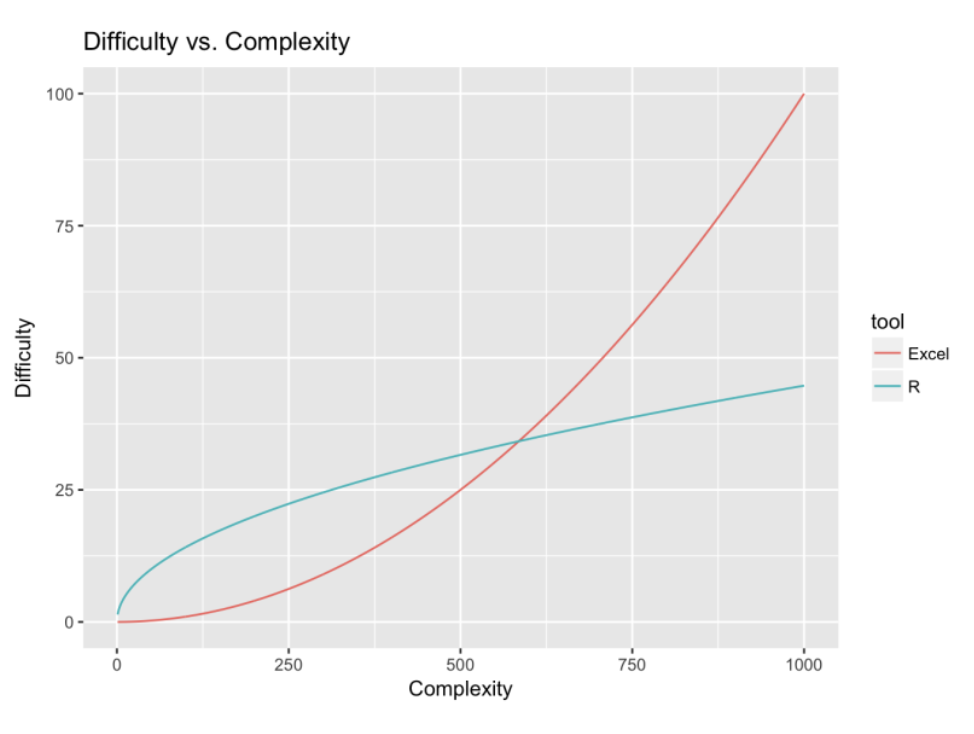
\includegraphics{images/rblogger.png}
Source: R-bloggers

\hypertarget{pourquoi-plus-excel}{%
\subsection{Pourquoi plus Excel ?}\label{pourquoi-plus-excel}}

Un exemple parmi tant d'autres !

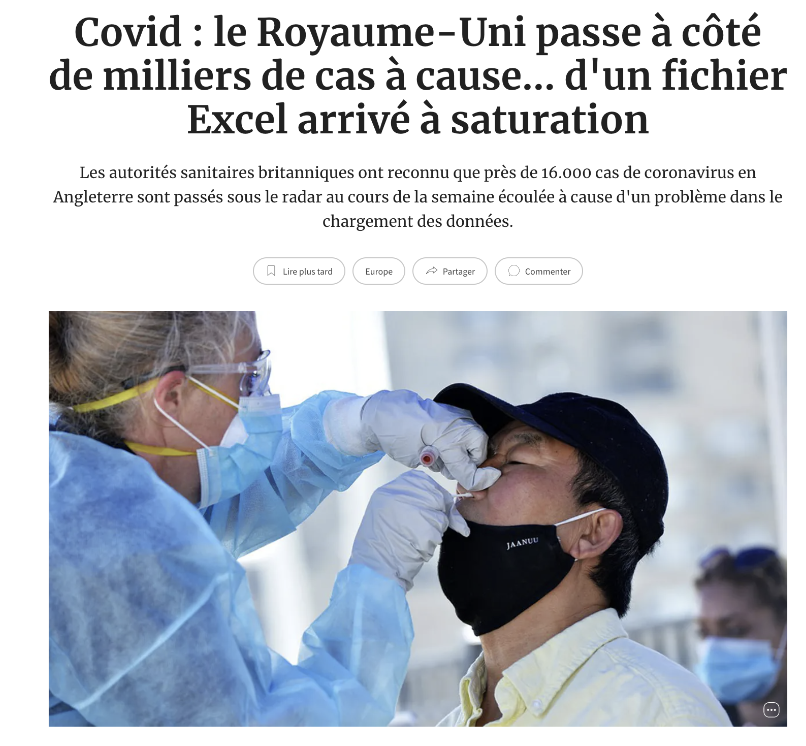
\includegraphics{images/covid.png}

Source Alexandre Counis, Les Echos, 5 oct. 2020

\hypertarget{avantages-et-inconvuxe9nients}{%
\section{Avantages et inconvénients}\label{avantages-et-inconvuxe9nients}}

\hypertarget{avantages}{%
\subsection{Avantages}\label{avantages}}

\begin{itemize}
\tightlist
\item
  Souplesse d'utilisation pour réaliser des analyses statistiques
\item
  Libre et gratuit, même s'il existe maintenant des versions payantes de RStudio (shiny et/ou server)
\item
  Reproductibilité des analyses en écrivant/sauvegardant les commandes R dans des scripts
\item
  Large communauté d'utilisateurs/aide en ligne
\item
  Grand nombre de packages spécifiques
\end{itemize}

\hypertarget{inconvuxe9nients}{%
\subsection{Inconvénients}\label{inconvuxe9nients}}

\hypertarget{geeks-and-repetitive-tasks}{%
\section{Geeks and repetitive tasks}\label{geeks-and-repetitive-tasks}}

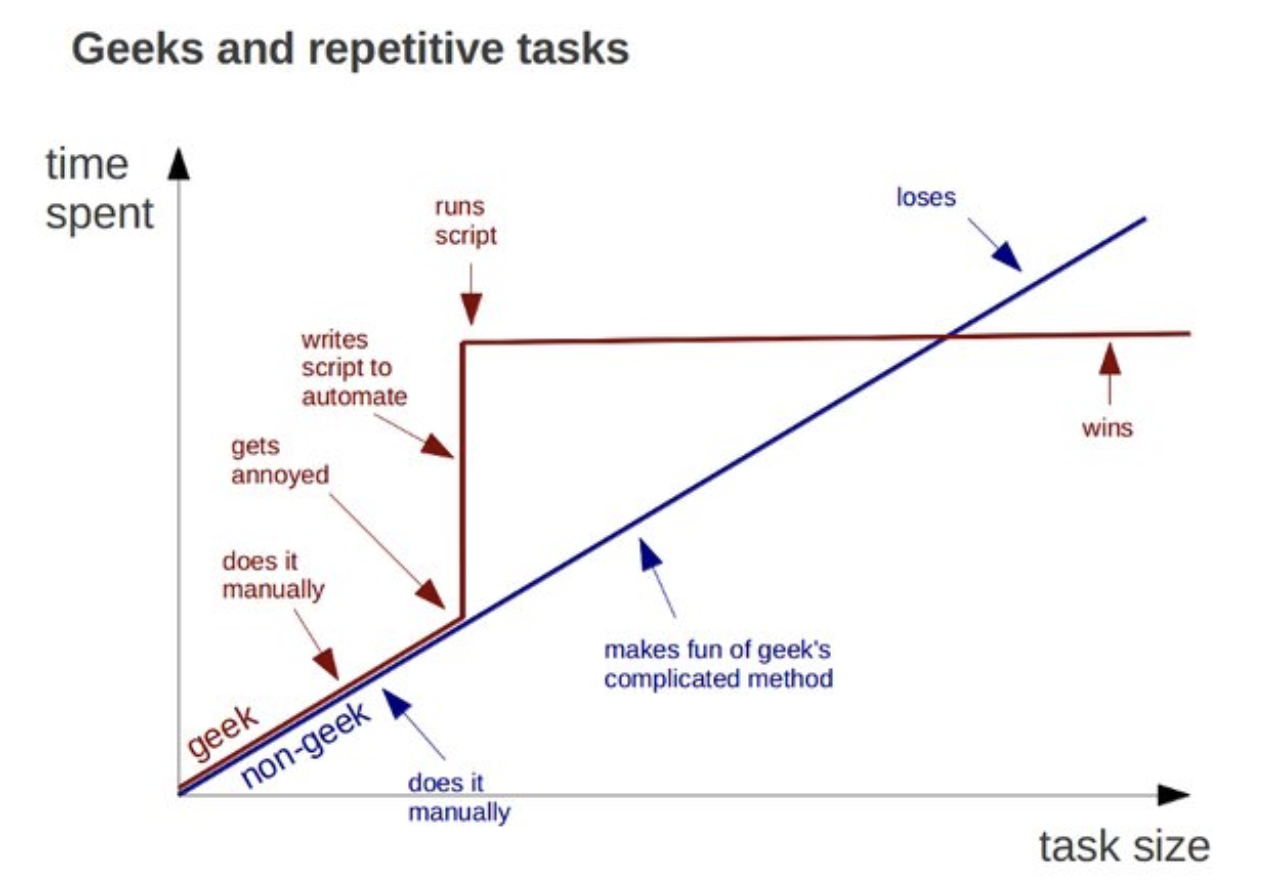
\includegraphics{images/geeks.png}

\hypertarget{r-sait-tout-faire}{%
\section{R sait tout faire}\label{r-sait-tout-faire}}

Lire un tableau de données

\begin{Shaded}
\begin{Highlighting}[]
\FunctionTok{read.table}\NormalTok{()}
\end{Highlighting}
\end{Shaded}

Fusionner deux tableaux

\begin{Shaded}
\begin{Highlighting}[]
\FunctionTok{merge}\NormalTok{()}
\end{Highlighting}
\end{Shaded}

Filtrer des lignes

\begin{Shaded}
\begin{Highlighting}[]
\NormalTok{data[data}\SpecialCharTok{$}\NormalTok{x }\SpecialCharTok{\textgreater{}} \DecValTok{10}\NormalTok{]}
\end{Highlighting}
\end{Shaded}

Sélectionner des colonnes

\begin{Shaded}
\begin{Highlighting}[]
\NormalTok{data[,}\FunctionTok{c}\NormalTok{(“x”,”y”)]}
\end{Highlighting}
\end{Shaded}

Rechercher une chaîne de caractères

\begin{Shaded}
\begin{Highlighting}[]
\FunctionTok{grep}\NormalTok{()}
\end{Highlighting}
\end{Shaded}

Réaliser une ACP

\begin{Shaded}
\begin{Highlighting}[]
\FunctionTok{prcomp}\NormalTok{()}
\end{Highlighting}
\end{Shaded}

Calculer une moyenne

\begin{Shaded}
\begin{Highlighting}[]
\FunctionTok{mean}\NormalTok{()}
\end{Highlighting}
\end{Shaded}

Additionner deux matrices

\begin{Shaded}
\begin{Highlighting}[]
\NormalTok{mat1 }\SpecialCharTok{+}\NormalTok{ mat2}
\end{Highlighting}
\end{Shaded}

Exporter un tableau de données

\begin{Shaded}
\begin{Highlighting}[]
\FunctionTok{write.table}\NormalTok{()}
\end{Highlighting}
\end{Shaded}

Calculer une variance

\begin{Shaded}
\begin{Highlighting}[]
\FunctionTok{var}\NormalTok{()}
\end{Highlighting}
\end{Shaded}

Régression linéaire

\begin{Shaded}
\begin{Highlighting}[]
\FunctionTok{lm}\NormalTok{()}
\end{Highlighting}
\end{Shaded}

Tracer une courbe

\begin{Shaded}
\begin{Highlighting}[]
\FunctionTok{plot}\NormalTok{()}
\end{Highlighting}
\end{Shaded}

Tester une hypothèse

\begin{Shaded}
\begin{Highlighting}[]
\FunctionTok{t.test}\NormalTok{()}
\end{Highlighting}
\end{Shaded}

Dessiner un histogramme

\begin{Shaded}
\begin{Highlighting}[]
\FunctionTok{hist}\NormalTok{()}
\end{Highlighting}
\end{Shaded}

Convertir des données

\begin{Shaded}
\begin{Highlighting}[]
\FunctionTok{as.matrix}\NormalTok{()}
\end{Highlighting}
\end{Shaded}

\hypertarget{comment-utiliser-r}{%
\chapter{Comment utiliser R ?}\label{comment-utiliser-r}}

\hypertarget{modes-dutilisation-liste-non-exhaustive}{%
\section{Modes d'utilisation (liste non exhaustive)}\label{modes-dutilisation-liste-non-exhaustive}}

\begin{itemize}
\tightlist
\item
  Localement via le terminal
\item
  Localement via RStudio (utilisation classique)
\item
  Sur un serveur via le terminal et une connexion ssh
\item
  Sur un serveur via un navigateur web pour accéder à RStudio server
\item
  Sur un serveur via un navigateur web pour accéder à RStudio server par Jupyter
\end{itemize}

\hypertarget{ouverture-ou-connexion-uxe0-rstudio}{%
\section{Ouverture ou connexion à RStudio}\label{ouverture-ou-connexion-uxe0-rstudio}}

3 alternatives :

\begin{enumerate}
\def\labelenumi{\arabic{enumi}.}
\item
  Ouvrir RStudio sur votre propre ordinateur (si installé)
\item
  Vous connecter au serveur Web RStudio de l'IFB
  \url{https://rstudio.cluster.france-bioinformatique.fr}
  puis vous identifier
\end{enumerate}

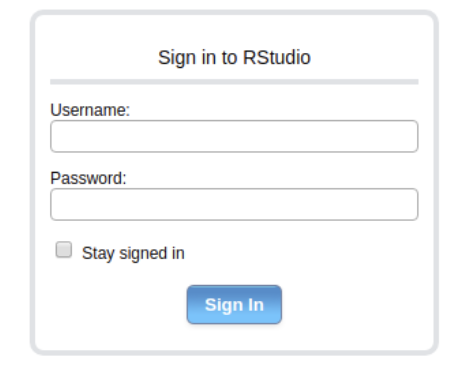
\includegraphics{images/coRstudio.png}

\begin{enumerate}
\def\labelenumi{\arabic{enumi}.}
\setcounter{enumi}{2}
\tightlist
\item
  Vous connecter via Jupyter lab de l'IFB
  \url{https://jupyterhub.cluster.france-bioinformatique.fr}
  puis cliquer sur l'icône RStudio
\end{enumerate}

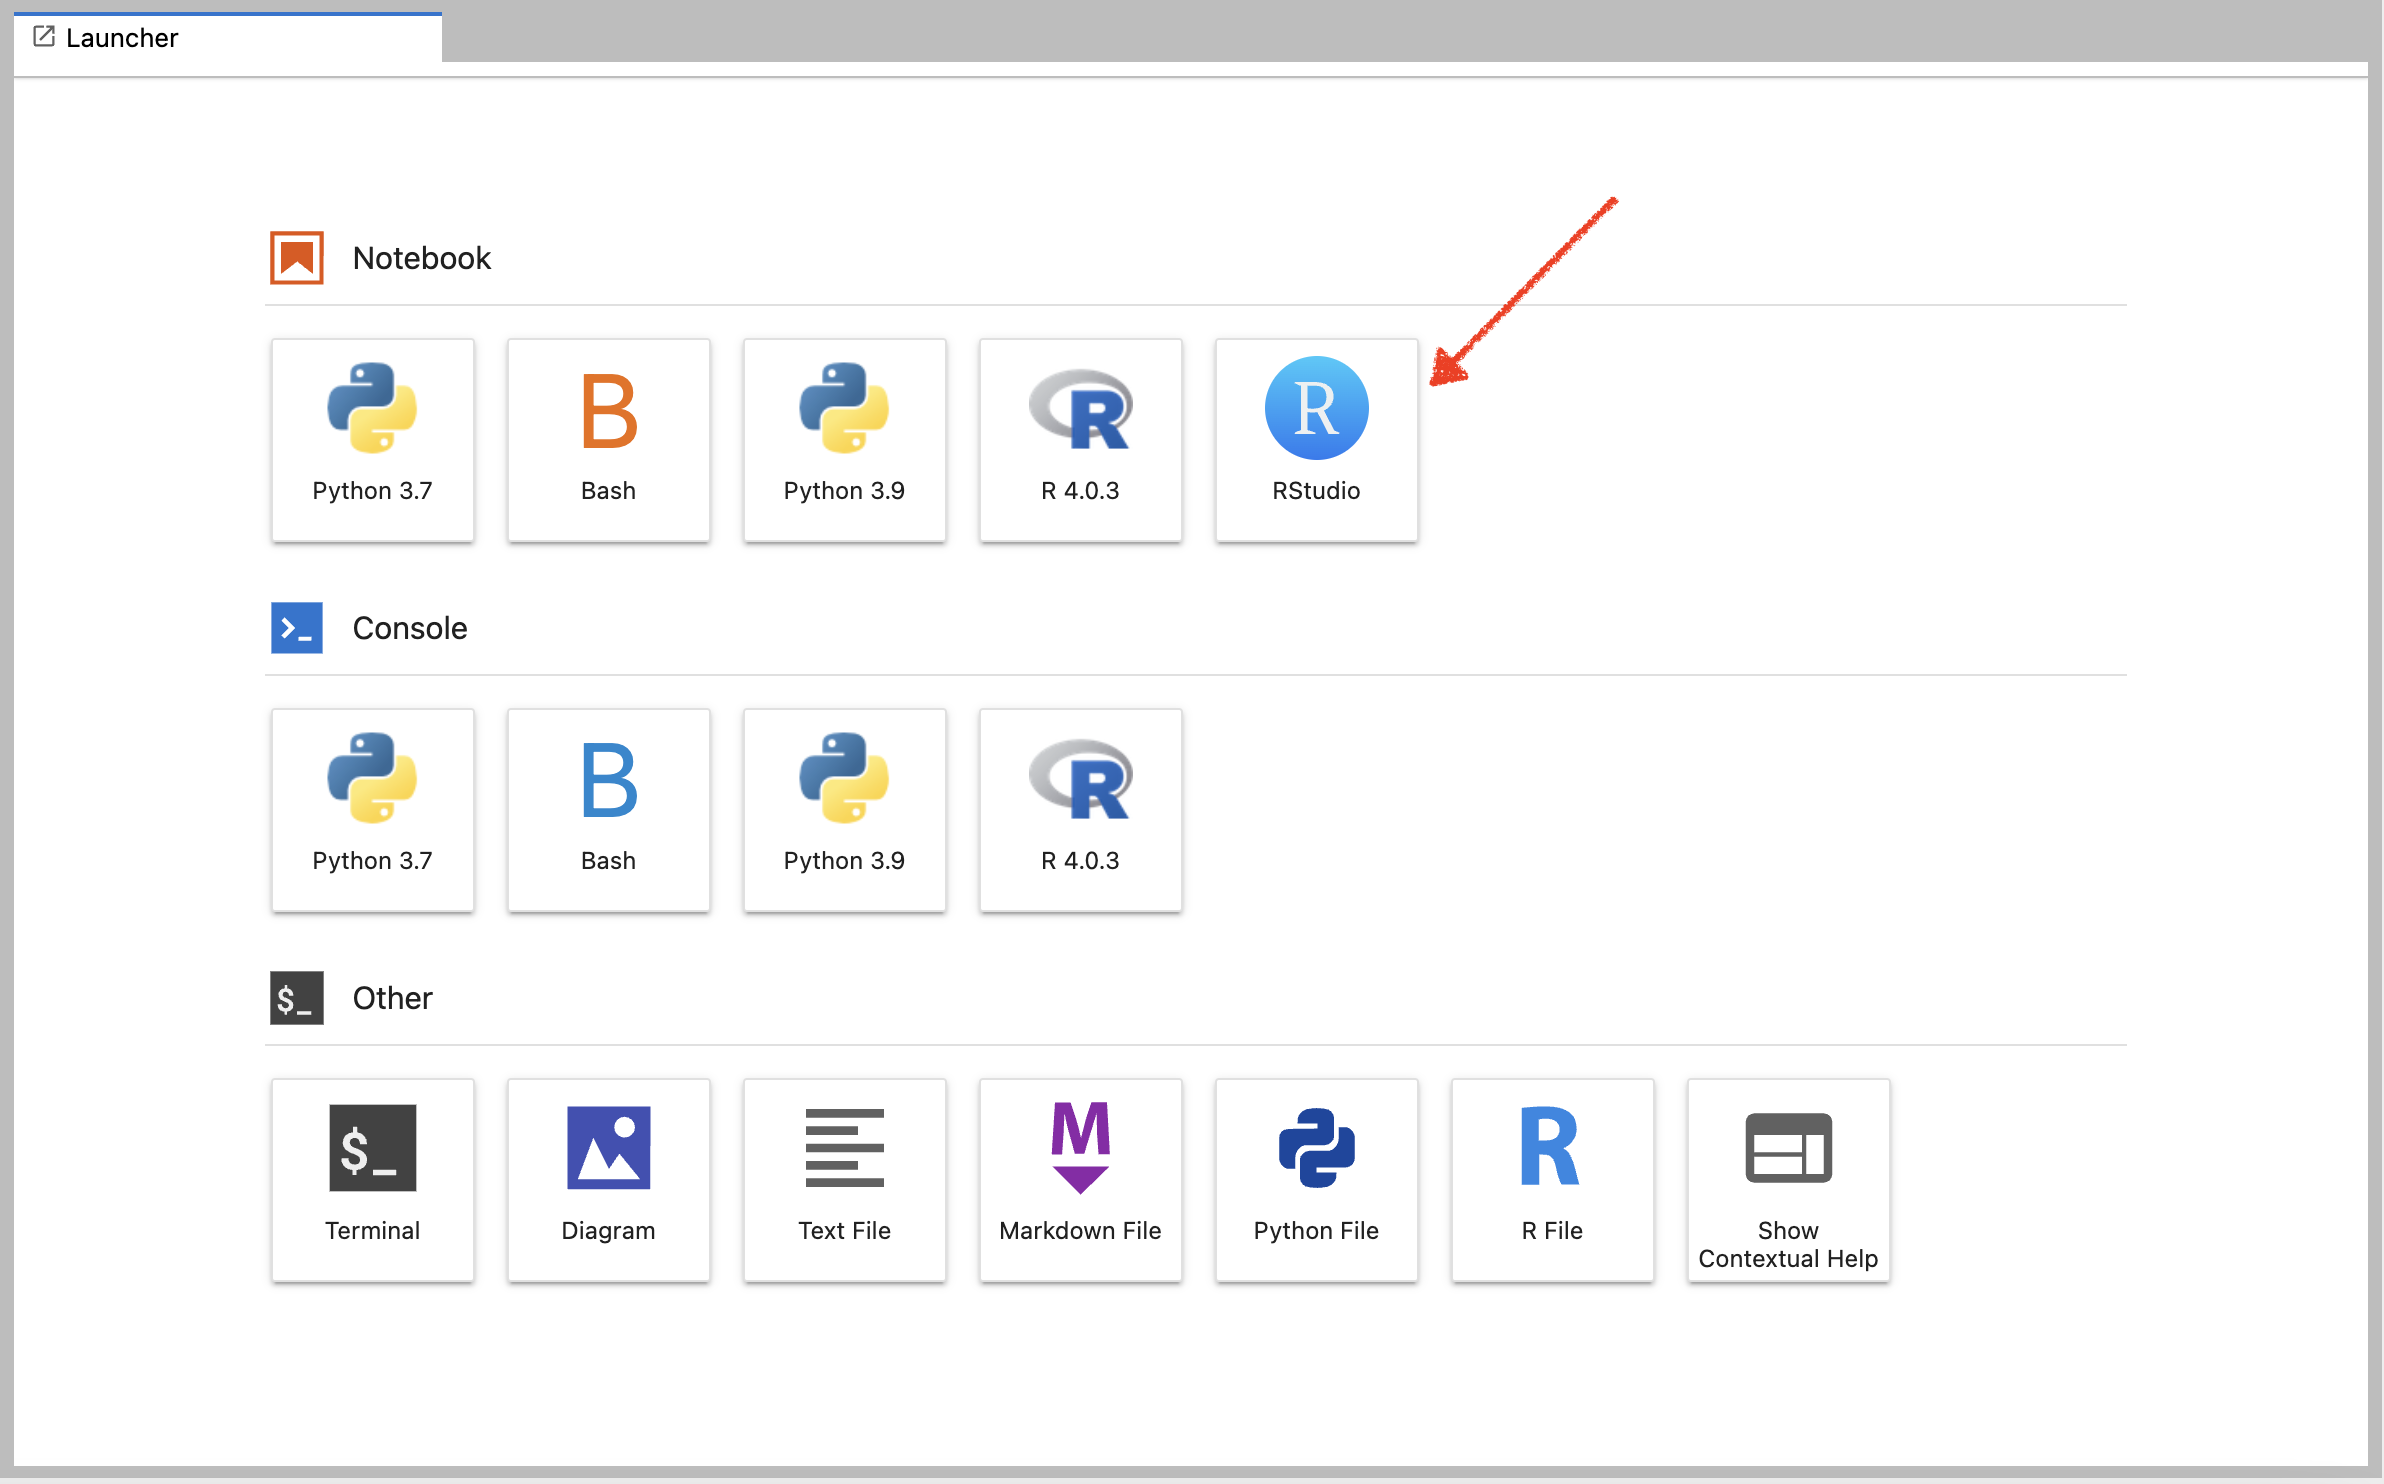
\includegraphics{images/jupyterRstudio.png}

\hypertarget{rstudio}{%
\section{RStudio}\label{rstudio}}

\begin{itemize}
\tightlist
\item
  Disponible depuis 2011
\item
  Logiciel facilitant l'utilisation de R via 4 panneaux
\item
  Chaque panneau présente plusieurs onglets (fonctionnalités complémentaires)
\end{itemize}

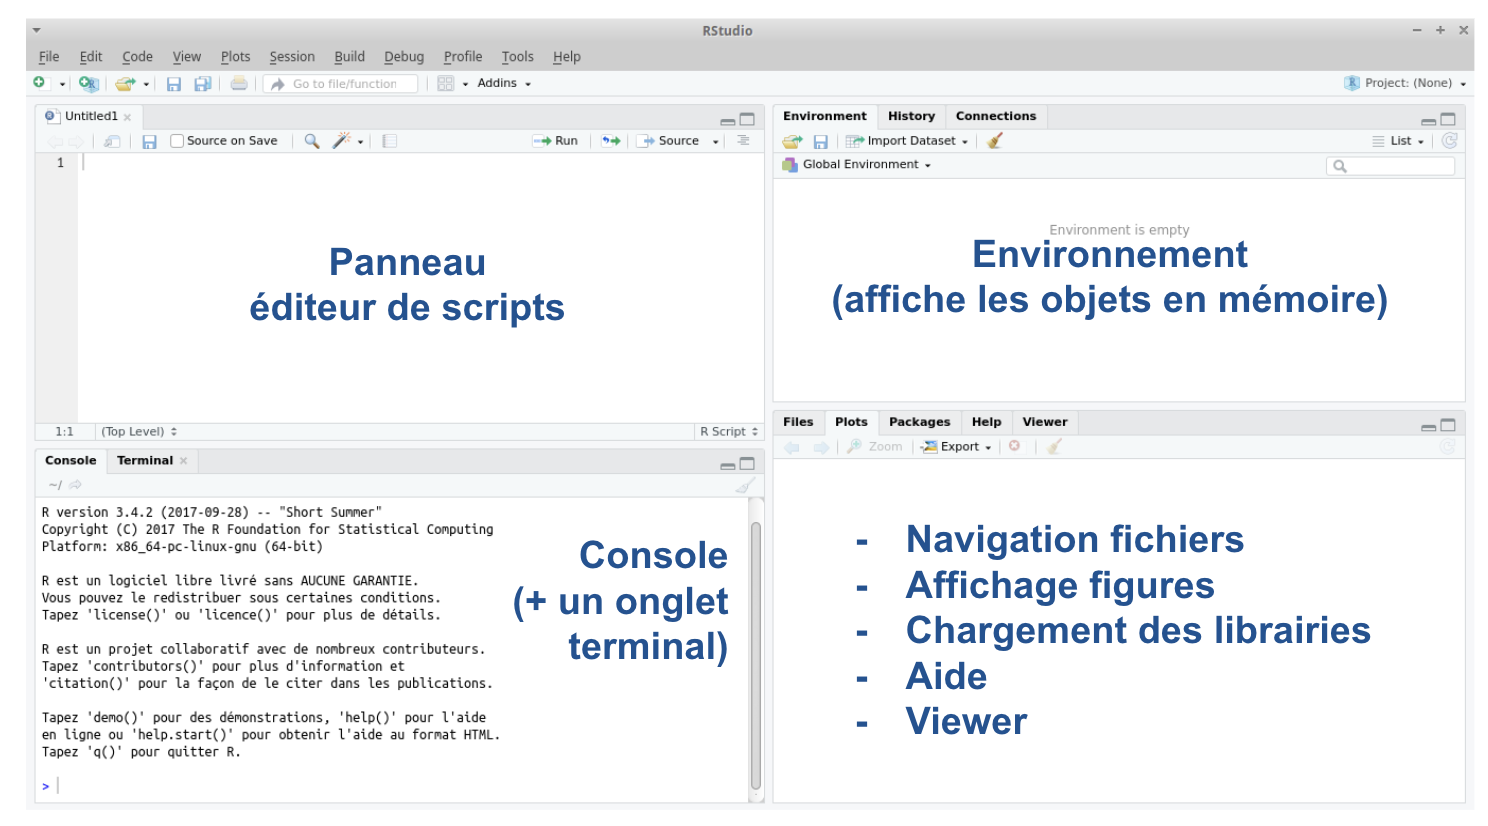
\includegraphics{images/rstudio.png}

\hypertarget{premiers-pas}{%
\chapter{Premiers pas}\label{premiers-pas}}

\hypertarget{r-sait-tout-faire-il-compte}{%
\section{R sait tout faire : il compte !}\label{r-sait-tout-faire-il-compte}}

Tapez les commandes suivantes dans le panneau Console de RStudio

\begin{Shaded}
\begin{Highlighting}[]
\DecValTok{2} \SpecialCharTok{+} \DecValTok{3}
\end{Highlighting}
\end{Shaded}

\begin{verbatim}
## [1] 5
\end{verbatim}

\begin{Shaded}
\begin{Highlighting}[]
\DecValTok{4} \SpecialCharTok{*} \DecValTok{5}
\end{Highlighting}
\end{Shaded}

\begin{verbatim}
## [1] 20
\end{verbatim}

\begin{Shaded}
\begin{Highlighting}[]
\DecValTok{6} \SpecialCharTok{/} \DecValTok{4}
\end{Highlighting}
\end{Shaded}

\begin{verbatim}
## [1] 1.5
\end{verbatim}

\begin{Shaded}
\begin{Highlighting}[]
\DecValTok{1}\SpecialCharTok{:}\DecValTok{10}
\end{Highlighting}
\end{Shaded}

\begin{verbatim}
##  [1]  1  2  3  4  5  6  7  8  9 10
\end{verbatim}

\begin{Shaded}
\begin{Highlighting}[]
\DecValTok{8}\SpecialCharTok{:{-}}\DecValTok{9}
\end{Highlighting}
\end{Shaded}

\begin{verbatim}
##  [1]  8  7  6  5  4  3  2  1  0 -1 -2 -3 -4 -5 -6 -7 -8 -9
\end{verbatim}

\begin{Shaded}
\begin{Highlighting}[]
\DecValTok{1}\NormalTok{,}\DecValTok{2}
\end{Highlighting}
\end{Shaded}

\begin{Shaded}
\begin{Highlighting}[]
\FloatTok{1.2}
\end{Highlighting}
\end{Shaded}

\begin{verbatim}
## [1] 1.2
\end{verbatim}

\hypertarget{notion-de-variableobjet}{%
\section{Notion de variable/objet}\label{notion-de-variableobjet}}

Créer une variable nommée a et lui assigner une valeur

\begin{Shaded}
\begin{Highlighting}[]
\NormalTok{a }\OtherTok{\textless{}{-}} \DecValTok{2}
\end{Highlighting}
\end{Shaded}

Afficher la valeur de la variable a

\begin{Shaded}
\begin{Highlighting}[]
\FunctionTok{print}\NormalTok{(a)}
\end{Highlighting}
\end{Shaded}

\begin{verbatim}
## [1] 2
\end{verbatim}

Même résultat: si on évoque le nom de variable, R l'imprime

\begin{Shaded}
\begin{Highlighting}[]
\NormalTok{a}
\end{Highlighting}
\end{Shaded}

\begin{verbatim}
## [1] 2
\end{verbatim}

Assigner une valeur à une seconde variable

\begin{Shaded}
\begin{Highlighting}[]
\NormalTok{b }\OtherTok{\textless{}{-}} \DecValTok{3}
\end{Highlighting}
\end{Shaded}

Effectuer un calcul avec 2 variables

\begin{Shaded}
\begin{Highlighting}[]
\NormalTok{a\_plus\_b }\OtherTok{\textless{}{-}}\NormalTok{ a }\SpecialCharTok{+}\NormalTok{ b}
\end{Highlighting}
\end{Shaded}

Afficher le contenu de la variable a\_plus\_b

\begin{Shaded}
\begin{Highlighting}[]
\FunctionTok{print}\NormalTok{(a\_plus\_b)}
\end{Highlighting}
\end{Shaded}

\begin{verbatim}
## [1] 5
\end{verbatim}

Changer la valeur de a

\begin{Shaded}
\begin{Highlighting}[]
\NormalTok{a }\OtherTok{\textless{}{-}} \DecValTok{7} 
\end{Highlighting}
\end{Shaded}

Note: le contenu de a\_plus\_b n'est pas modifié

\begin{Shaded}
\begin{Highlighting}[]
\FunctionTok{print}\NormalTok{(a\_plus\_b) }
\end{Highlighting}
\end{Shaded}

\begin{verbatim}
## [1] 5
\end{verbatim}

On recalcule a\_plus\_b

\begin{Shaded}
\begin{Highlighting}[]
\NormalTok{a\_plus\_b }\OtherTok{\textless{}{-}}\NormalTok{ a }\SpecialCharTok{+}\NormalTok{ b }
\end{Highlighting}
\end{Shaded}

La nouvelle valeur tient compte de la modification de a

\begin{Shaded}
\begin{Highlighting}[]
\FunctionTok{print}\NormalTok{(a\_plus\_b)}
\end{Highlighting}
\end{Shaded}

\begin{verbatim}
## [1] 10
\end{verbatim}

Créer un vecteur

\begin{Shaded}
\begin{Highlighting}[]
\NormalTok{vec1 }\OtherTok{\textless{}{-}}  \FunctionTok{c}\NormalTok{(}\DecValTok{1}\NormalTok{,}\DecValTok{10}\NormalTok{)}
\end{Highlighting}
\end{Shaded}

Créer un vecteur contenant une séquence d'entiers de 1 à 10

\begin{Shaded}
\begin{Highlighting}[]
\NormalTok{vec2 }\OtherTok{\textless{}{-}}  \DecValTok{1}\SpecialCharTok{:}\DecValTok{10}
\end{Highlighting}
\end{Shaded}

Somme d'un vecteur et d'un nombre

\begin{Shaded}
\begin{Highlighting}[]
\NormalTok{vec2 }\SpecialCharTok{+}\NormalTok{ a }
\end{Highlighting}
\end{Shaded}

\begin{verbatim}
##  [1]  8  9 10 11 12 13 14 15 16 17
\end{verbatim}

Vecteur de chaînes de caractères

\begin{Shaded}
\begin{Highlighting}[]
\NormalTok{vec3 }\OtherTok{\textless{}{-}}  \FunctionTok{c}\NormalTok{(}\StringTok{"riri"}\NormalTok{, }\StringTok{"fifi"}\NormalTok{, }\StringTok{"loulou"}\NormalTok{)}
\end{Highlighting}
\end{Shaded}

Diviser un vecteur de nombres par un nombre

\begin{Shaded}
\begin{Highlighting}[]
\NormalTok{vec2 }\SpecialCharTok{/} \DecValTok{2}
\end{Highlighting}
\end{Shaded}

\begin{verbatim}
##  [1] 0.5 1.0 1.5 2.0 2.5 3.0 3.5 4.0 4.5 5.0
\end{verbatim}

Diviser des chaînes de caractères par un nombre

\begin{Shaded}
\begin{Highlighting}[]
\NormalTok{vec3  }\SpecialCharTok{/} \DecValTok{2}   
\end{Highlighting}
\end{Shaded}

\textbf{Attention} : Noms de variables interdits: TRUE, FALSE, T, F, c, t, pi, data, LETTERS, letters, \ldots{}

\hypertarget{import-de-donnuxe9es}{%
\chapter{Import de données}\label{import-de-donnuxe9es}}

\hypertarget{version-avec-les-boutons}{%
\section{Version ``Avec les boutons''}\label{version-avec-les-boutons}}

\hypertarget{cruxe9ation-dun-dossier-intro_r-pour-vos-ruxe9sultats-de-ce-tp}{%
\subsection{Création d'un dossier intro\_R pour vos résultats de ce TP}\label{cruxe9ation-dun-dossier-intro_r-pour-vos-ruxe9sultats-de-ce-tp}}

\textbf{Attention} Dans votre espace projet ou votre home.

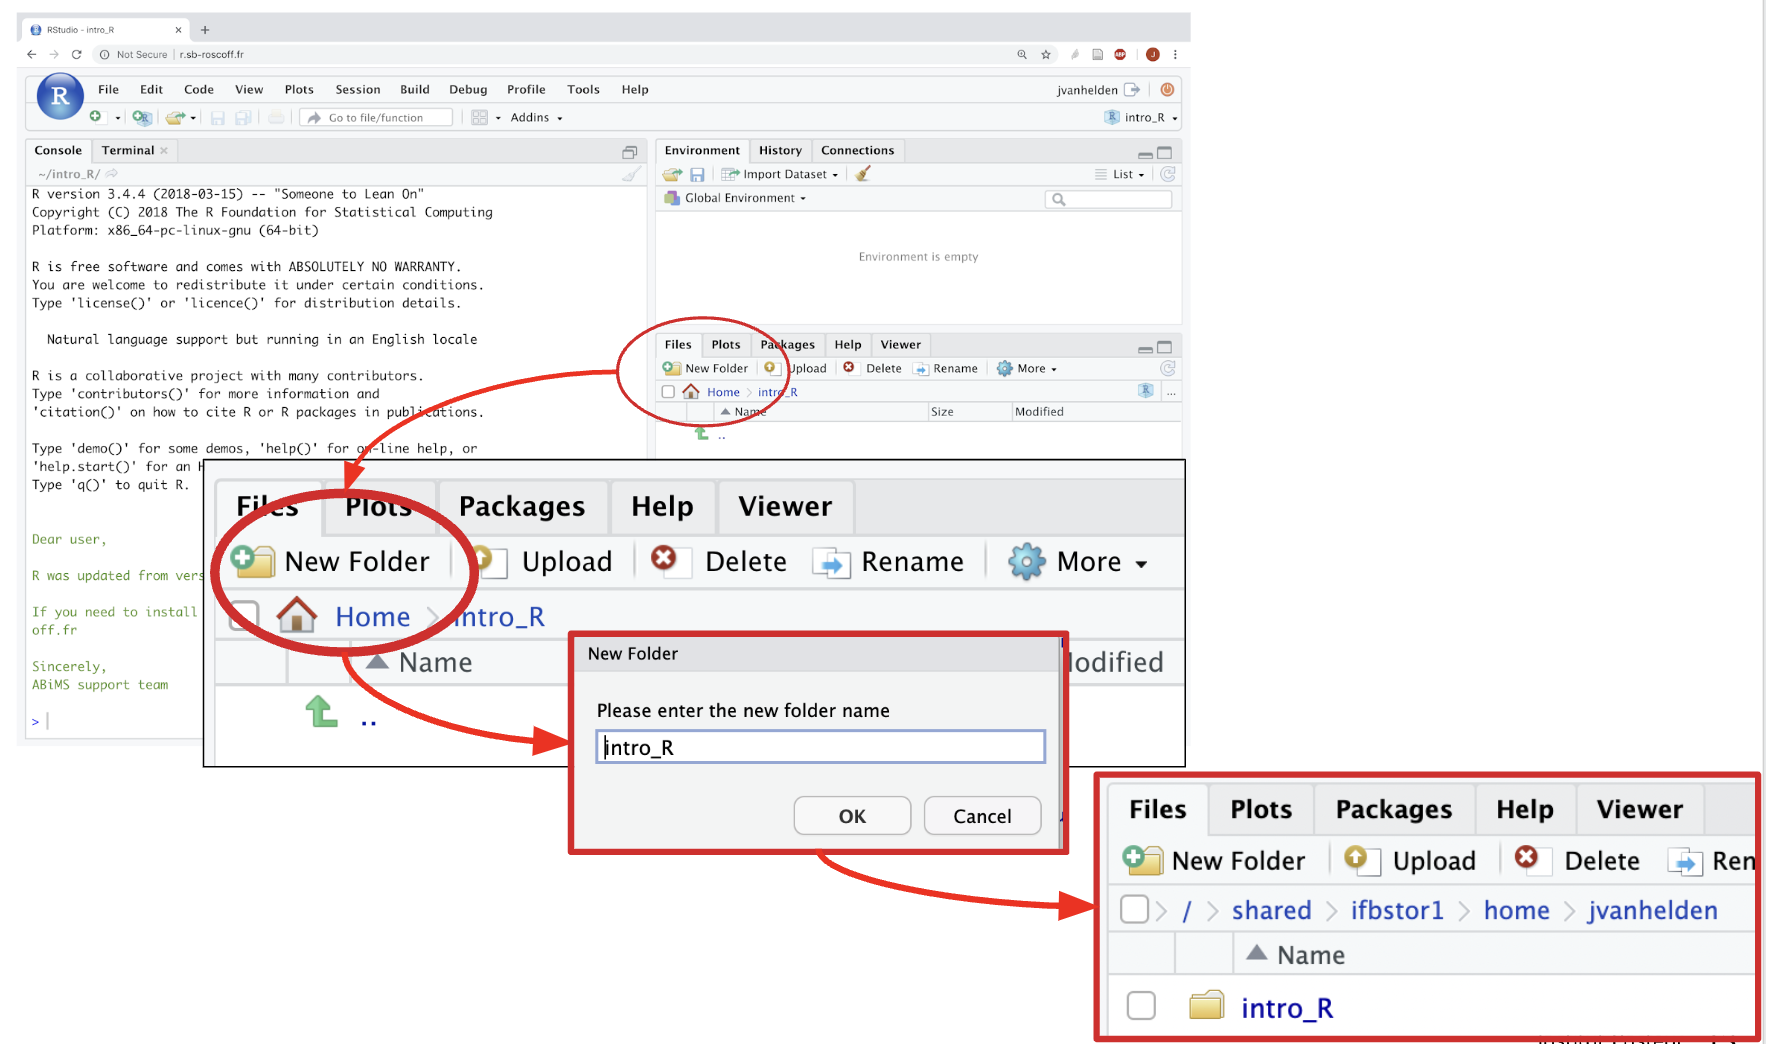
\includegraphics{images/createIntro.png}

\hypertarget{duxe9placement-dans-le-dossier-intro_r}{%
\subsection{Déplacement dans le dossier ``intro\_R''}\label{duxe9placement-dans-le-dossier-intro_r}}

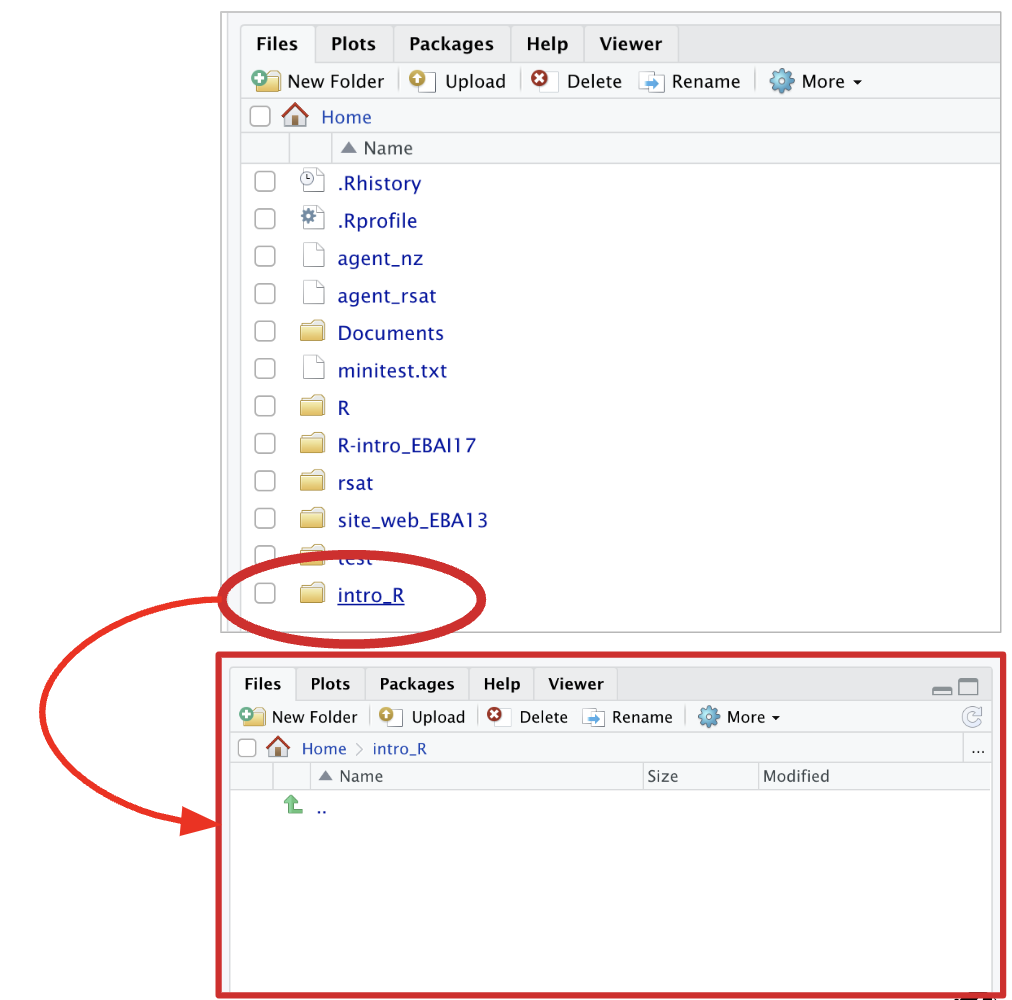
\includegraphics{images/moveIntro.png}

\hypertarget{duxe9finissez-votre-dossier-espace-de-travail-working-directory}{%
\subsection{Définissez votre dossier espace de travail (working directory)}\label{duxe9finissez-votre-dossier-espace-de-travail-working-directory}}

\begin{enumerate}
\def\labelenumi{\arabic{enumi}.}
\tightlist
\item
  Dans le menu ``Session'', lancez ``Choose Directory \ldots{}''
\item
  Naviguez jusqu'à votre dossier intro\_R
\item
  Double-cliquez dessus pour l'ouvrir
\item
  Cliquez Choose
\end{enumerate}

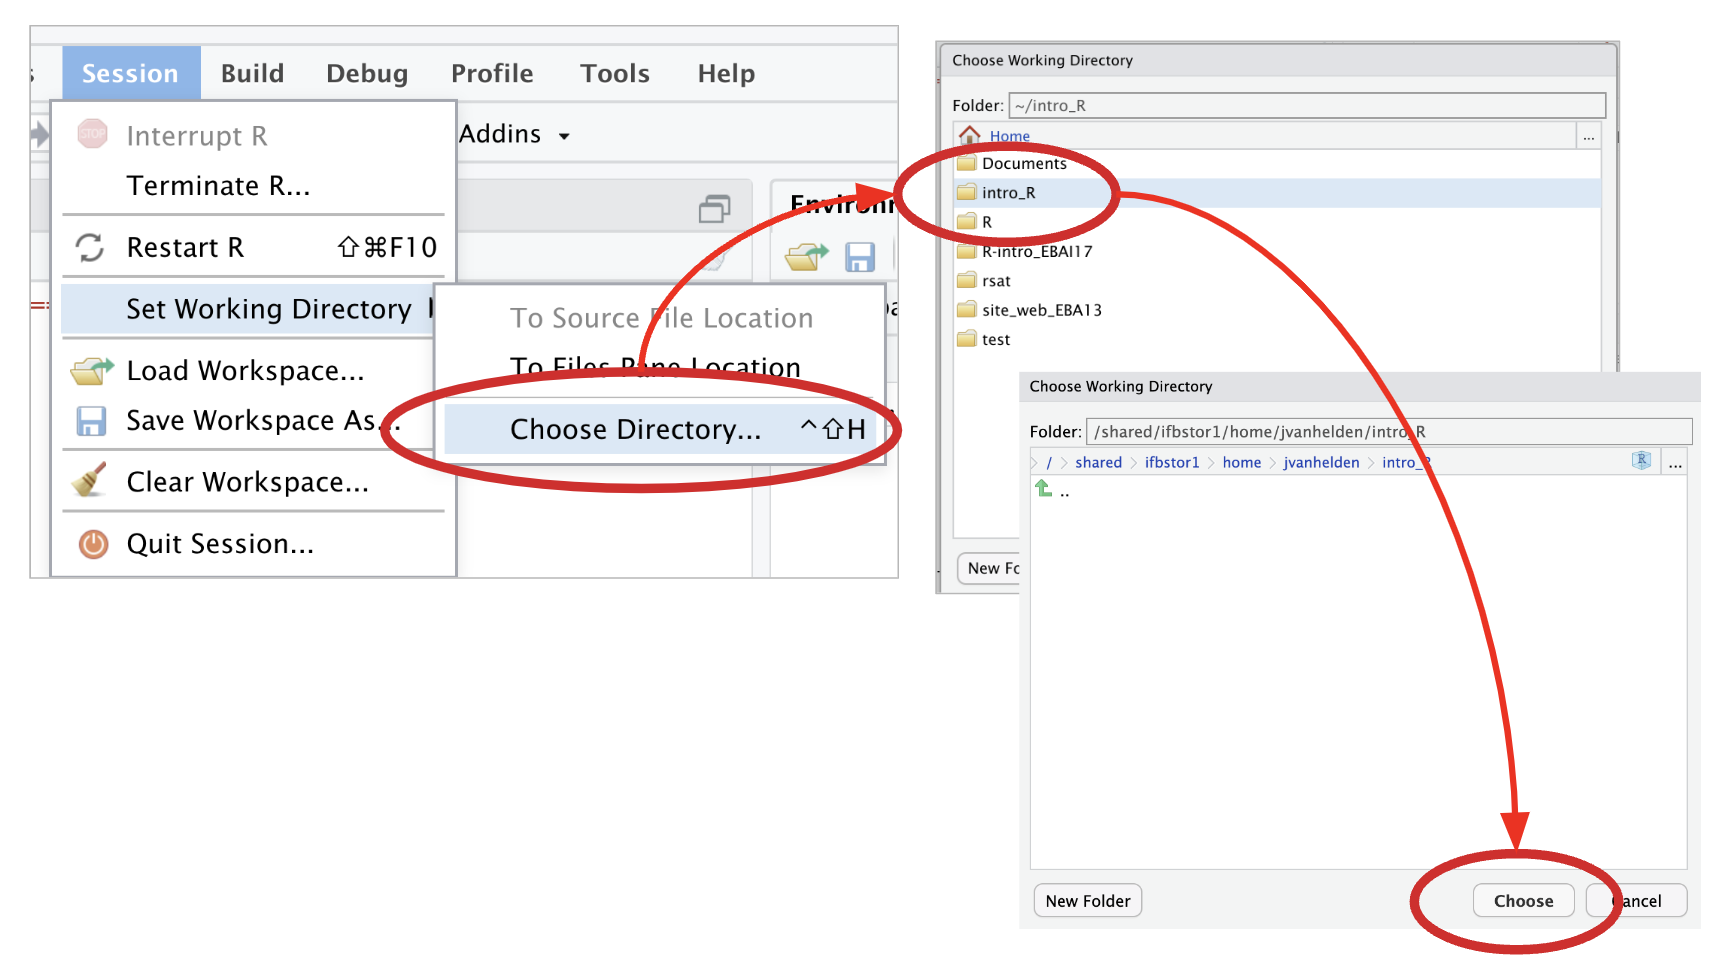
\includegraphics{images/setWd.png}

\hypertarget{tuxe9luxe9chargez-les-fichiers-sur-votre-machine}{%
\subsection{Téléchargez les fichiers sur votre machine}\label{tuxe9luxe9chargez-les-fichiers-sur-votre-machine}}

A partir d'un navigateur Web, téléchargez et enregistrez sur votre ordi les fichiers de données
- \href{https://raw.githubusercontent.com/IFB-ElixirFr/EBAII/master/2022/ebaiin1/intro_R/expression.txt}{expression.txt}: données d'expressions pour 4 échantillons
- \href{https://raw.githubusercontent.com/IFB-ElixirFr/EBAII/master/2022/ebaiin1/intro_R/annotation.csv}{annotation.csv}: informations sur les gènes (id, name, chr, start, stop)

Attention: veillez à sauvegarder les fichiers
- sous leur nom original,
- avec les extensions .txt et .csv respectives (certains navigateurs omettent l'extension, ce qui poserait problème pour la suite du TP)

\hypertarget{tuxe9luxe9versement-upload-des-donnuxe9es}{%
\subsection{Téléversement (``upload'') des données}\label{tuxe9luxe9versement-upload-des-donnuxe9es}}

Au moyen du bouton ``Upload'', téléversez les fichiers d'expression et d'annotation depuis votre ordinateur vers votre compte sur le serveur.

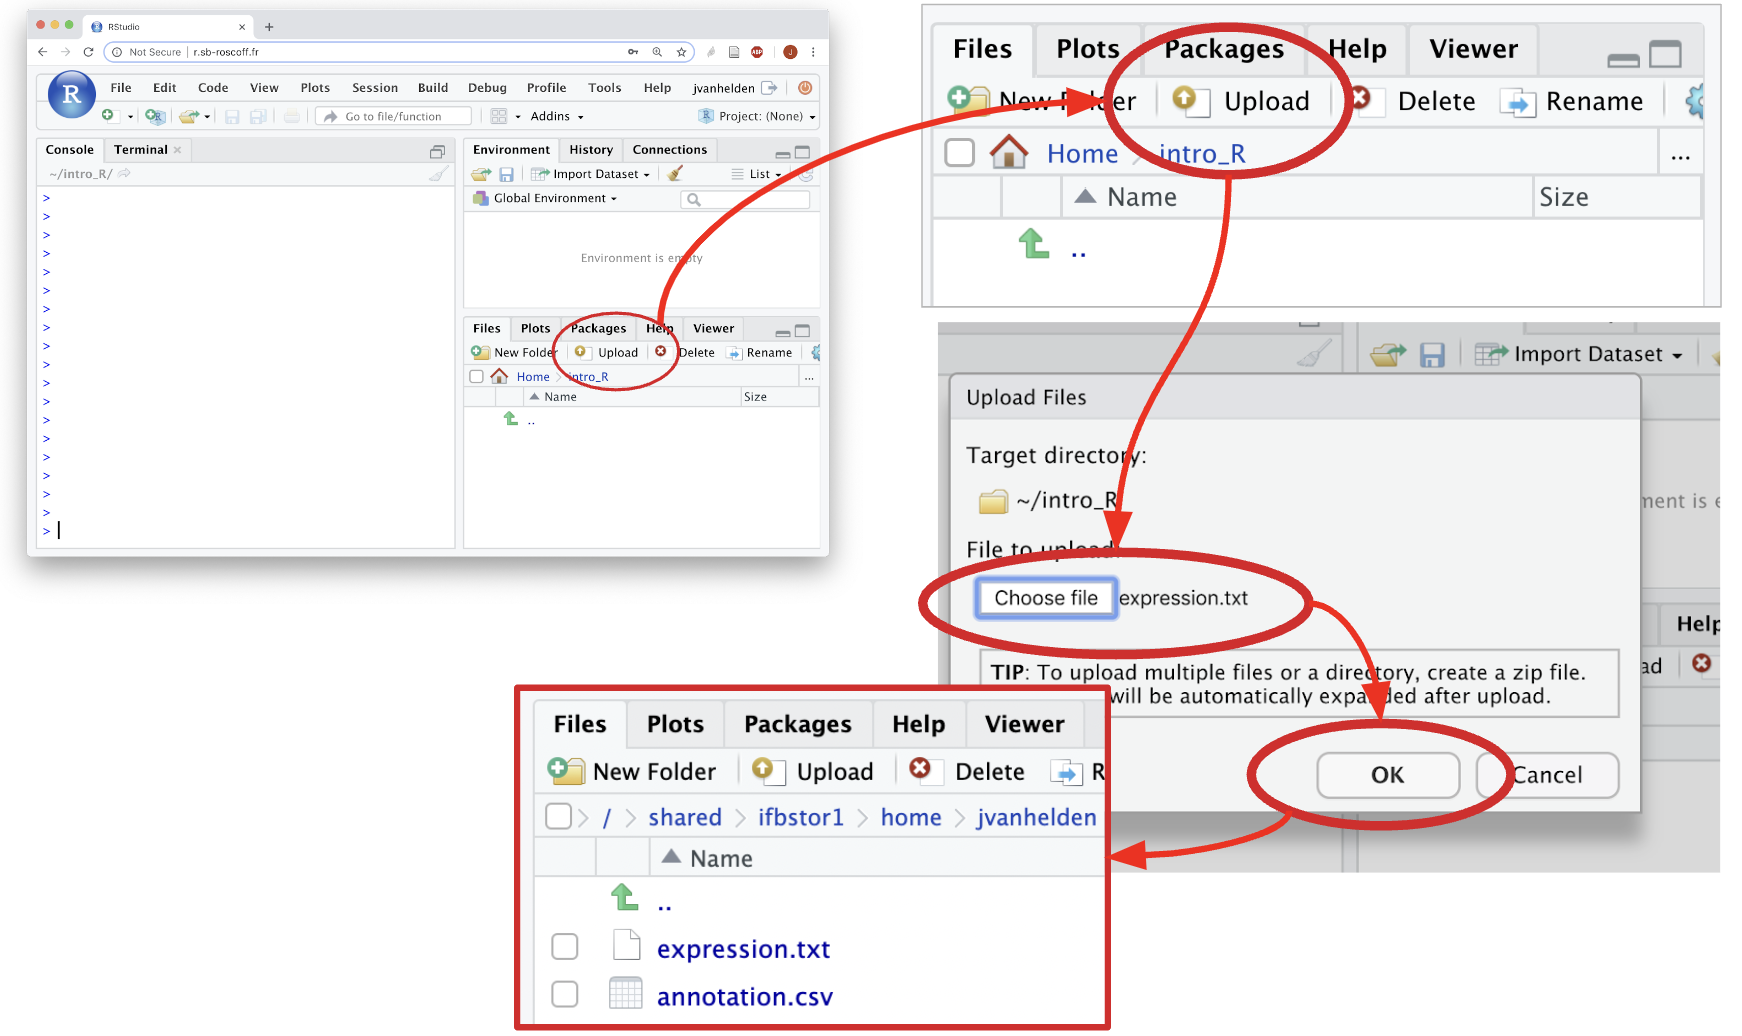
\includegraphics{images/uploadData.png}

\hypertarget{on-efface-tout-et-on-recommence}{%
\subsection{On efface tout et on recommence}\label{on-efface-tout-et-on-recommence}}

\begin{enumerate}
\def\labelenumi{\arabic{enumi}.}
\tightlist
\item
  Sélectionnez les deux fichiers
\item
  Effacez-les sans pitié
\end{enumerate}

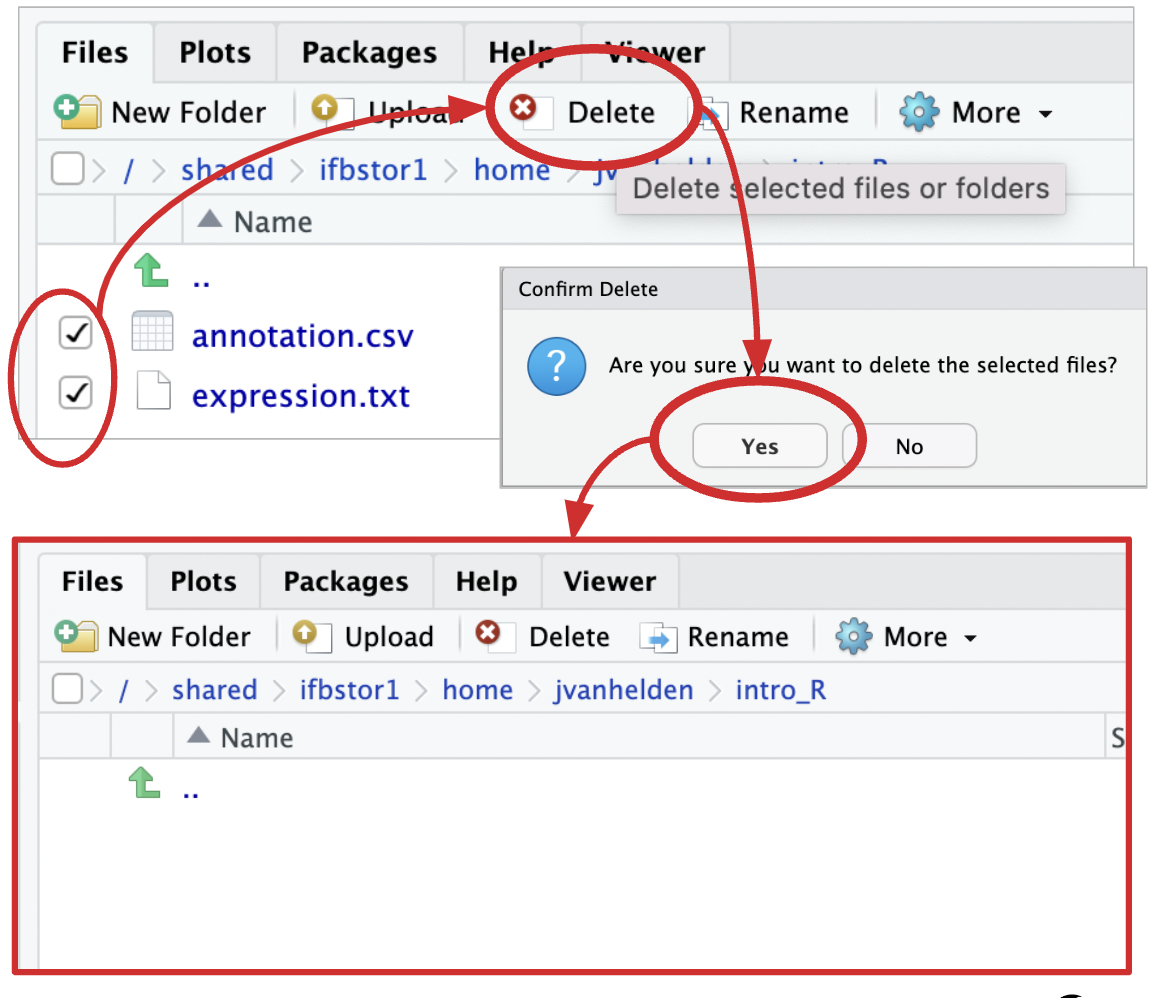
\includegraphics{images/delete.png}

(nous allons vous montrer deux autres façons de les téléverser)

\hypertarget{the-r-geek-way-v2-directement-depuis-rstudio}{%
\section{The ``R geek'' way (V2, directement depuis Rstudio)}\label{the-r-geek-way-v2-directement-depuis-rstudio}}

Attention ! Dans votre espace projet !

\hypertarget{creation-de-larborescence}{%
\subsection{Creation de l'arborescence}\label{creation-de-larborescence}}

Aller dans \textbf{votre} espace projet !

Dans tous les commandes ci-dessous, remplacer toujours \texttt{form\_2022\_32/EBAII\_IntroR} par votre nom d'espace projet

Note : Pour les personnes ne travaillant pas sur le cluster mais par exemple en local, vous pouvez sans soucis remplacer l'adresse par une adresse sur votre ordinateur.

\begin{Shaded}
\begin{Highlighting}[]
\FunctionTok{setwd}\NormalTok{(}\StringTok{"/shared/ifbstor1/projects/form\_2022\_32/EBAII\_IntroR"}\NormalTok{)}
\end{Highlighting}
\end{Shaded}

Définir une variable qui indique le chemin du dossier de travail (working directory).

\begin{Shaded}
\begin{Highlighting}[]
\NormalTok{my\_work\_dir }\OtherTok{\textless{}{-}} \StringTok{"/shared/ifbstor1/projects/form\_2022\_32/EBAII\_IntroR/intro\_R"} 
\end{Highlighting}
\end{Shaded}

S'il n'existe pas encore, créer le dossier de travail. (Commande Unix équivalente: \texttt{mkdir\ -p\ /shared/ifbstor1/projects/form\_2022\_32/EBAII\_IntroR/intro\_R})

\begin{Shaded}
\begin{Highlighting}[]
\FunctionTok{dir.create}\NormalTok{(my\_work\_dir, }\AttributeTok{recursive =} \ConstantTok{TRUE}\NormalTok{, }\AttributeTok{showWarnings =} \ConstantTok{FALSE}\NormalTok{)}
\end{Highlighting}
\end{Shaded}

Où suis-je ? (Commande Unix équivalente: \texttt{pwd})

\begin{Shaded}
\begin{Highlighting}[]
\FunctionTok{getwd}\NormalTok{()}
\end{Highlighting}
\end{Shaded}

\begin{verbatim}
## [1] "/shared/ifbstor1/projects/form_2022_32/EBAII_IntroR"
\end{verbatim}

Aller dans ce dossier de travail (Commande Unix équivalente: \texttt{cd\ /shared/ifbstor1/projects/form\_2022\_32/EBAII\_IntroR/intro\_R})

\begin{Shaded}
\begin{Highlighting}[]
\FunctionTok{setwd}\NormalTok{(my\_work\_dir)}
\end{Highlighting}
\end{Shaded}

Et maintenant, où suis-je ?

\begin{Shaded}
\begin{Highlighting}[]
\FunctionTok{getwd}\NormalTok{()}
\end{Highlighting}
\end{Shaded}

\begin{verbatim}
## [1] "/shared/ifbstor1/projects/form_2022_32/EBAII_IntroR"
\end{verbatim}

Qu'y a-t-il par ici ? (Commande Unix équivalente: \texttt{ls})

\begin{Shaded}
\begin{Highlighting}[]
\FunctionTok{list.files}\NormalTok{()}
\end{Highlighting}
\end{Shaded}

\begin{verbatim}
##  [1] "_bookdown_files"    "_bookdown.yml"      "_main_files"       
##  [4] "_main.log"          "_main.pdf"          "_main.Rmd"         
##  [7] "_main.tex"          "_output.yml"        "01-intro.Rmd"      
## [10] "02-how.Rmd"         "03-firstSteps.Rmd"  "04-uploadData.Rmd" 
## [13] "05-readData.Rmd"    "06-manipulate.Rmd"  "07-plots.Rmd"      
## [16] "08-analyseDiff.Rmd" "09-integration.Rmd" "10-visu.Rmd"       
## [19] "11-conclusion.Rmd"  "12-references.Rmd"  "annotation.csv"    
## [22] "book.bib"           "docs"               "EBAII_IntroR.Rproj"
## [25] "expression.txt"     "exprs_chr8.txt"     "images"            
## [28] "index.Rmd"          "intro_R"            "LICENSE"           
## [31] "packages.bib"       "preamble.tex"       "README.md"         
## [34] "style.css"
\end{verbatim}

Un autre nom pour la même commande

\begin{Shaded}
\begin{Highlighting}[]
\FunctionTok{dir}\NormalTok{()}
\end{Highlighting}
\end{Shaded}

\begin{verbatim}
##  [1] "_bookdown_files"    "_bookdown.yml"      "_main_files"       
##  [4] "_main.log"          "_main.pdf"          "_main.Rmd"         
##  [7] "_main.tex"          "_output.yml"        "01-intro.Rmd"      
## [10] "02-how.Rmd"         "03-firstSteps.Rmd"  "04-uploadData.Rmd" 
## [13] "05-readData.Rmd"    "06-manipulate.Rmd"  "07-plots.Rmd"      
## [16] "08-analyseDiff.Rmd" "09-integration.Rmd" "10-visu.Rmd"       
## [19] "11-conclusion.Rmd"  "12-references.Rmd"  "annotation.csv"    
## [22] "book.bib"           "docs"               "EBAII_IntroR.Rproj"
## [25] "expression.txt"     "exprs_chr8.txt"     "images"            
## [28] "index.Rmd"          "intro_R"            "LICENSE"           
## [31] "packages.bib"       "preamble.tex"       "README.md"         
## [34] "style.css"
\end{verbatim}

\hypertarget{tuxe9luxe9charger-un-fichier}{%
\subsection{Télécharger un fichier}\label{tuxe9luxe9charger-un-fichier}}

Nous avons montré ci-dessus comment télécharger des fichiers en utilisant l'interface graphique de RStudio.

Alternativement, on peut télécharger des fichiers au moyen de la commande R download.file.

Les deux commandes suivantes permettent de télécharger les fichiers utilisés pour les exercices.

\begin{Shaded}
\begin{Highlighting}[]
\FunctionTok{download.file}\NormalTok{(}\AttributeTok{url =} \StringTok{"https://raw.githubusercontent.com/IFB{-}ElixirFr/EBAII/master/2022/ebaiin1/intro\_R/expression.txt"}\NormalTok{, }\AttributeTok{destfile =} \StringTok{"expression.txt"}\NormalTok{)}
\end{Highlighting}
\end{Shaded}

\begin{Shaded}
\begin{Highlighting}[]
\FunctionTok{download.file}\NormalTok{(}\AttributeTok{url =} \StringTok{"https://raw.githubusercontent.com/IFB{-}ElixirFr/EBAII/master/2022/ebaiin1/intro\_R/annotation.csv"}\NormalTok{, }\AttributeTok{destfile =} \StringTok{"annotation.csv"}\NormalTok{)}
\end{Highlighting}
\end{Shaded}

Note : équivalent de la commande \texttt{wget} sous Unix.

Qu'y a-t-il par ici ? (Commande Unix équivalente: \texttt{ls})

\begin{Shaded}
\begin{Highlighting}[]
\FunctionTok{list.files}\NormalTok{()}
\end{Highlighting}
\end{Shaded}

\begin{verbatim}
##  [1] "_bookdown_files"    "_bookdown.yml"      "_main_files"       
##  [4] "_main.log"          "_main.pdf"          "_main.Rmd"         
##  [7] "_main.tex"          "_output.yml"        "01-intro.Rmd"      
## [10] "02-how.Rmd"         "03-firstSteps.Rmd"  "04-uploadData.Rmd" 
## [13] "05-readData.Rmd"    "06-manipulate.Rmd"  "07-plots.Rmd"      
## [16] "08-analyseDiff.Rmd" "09-integration.Rmd" "10-visu.Rmd"       
## [19] "11-conclusion.Rmd"  "12-references.Rmd"  "annotation.csv"    
## [22] "book.bib"           "docs"               "EBAII_IntroR.Rproj"
## [25] "expression.txt"     "exprs_chr8.txt"     "images"            
## [28] "index.Rmd"          "intro_R"            "LICENSE"           
## [31] "packages.bib"       "preamble.tex"       "README.md"         
## [34] "style.css"
\end{verbatim}

\hypertarget{on-efface-tout-et-on-recommence-1}{%
\subsection{On efface tout et on recommence}\label{on-efface-tout-et-on-recommence-1}}

\begin{enumerate}
\def\labelenumi{\arabic{enumi}.}
\tightlist
\item
  Sélectionnez les deux fichiers
\item
  Effacez-les sans pitié
\end{enumerate}

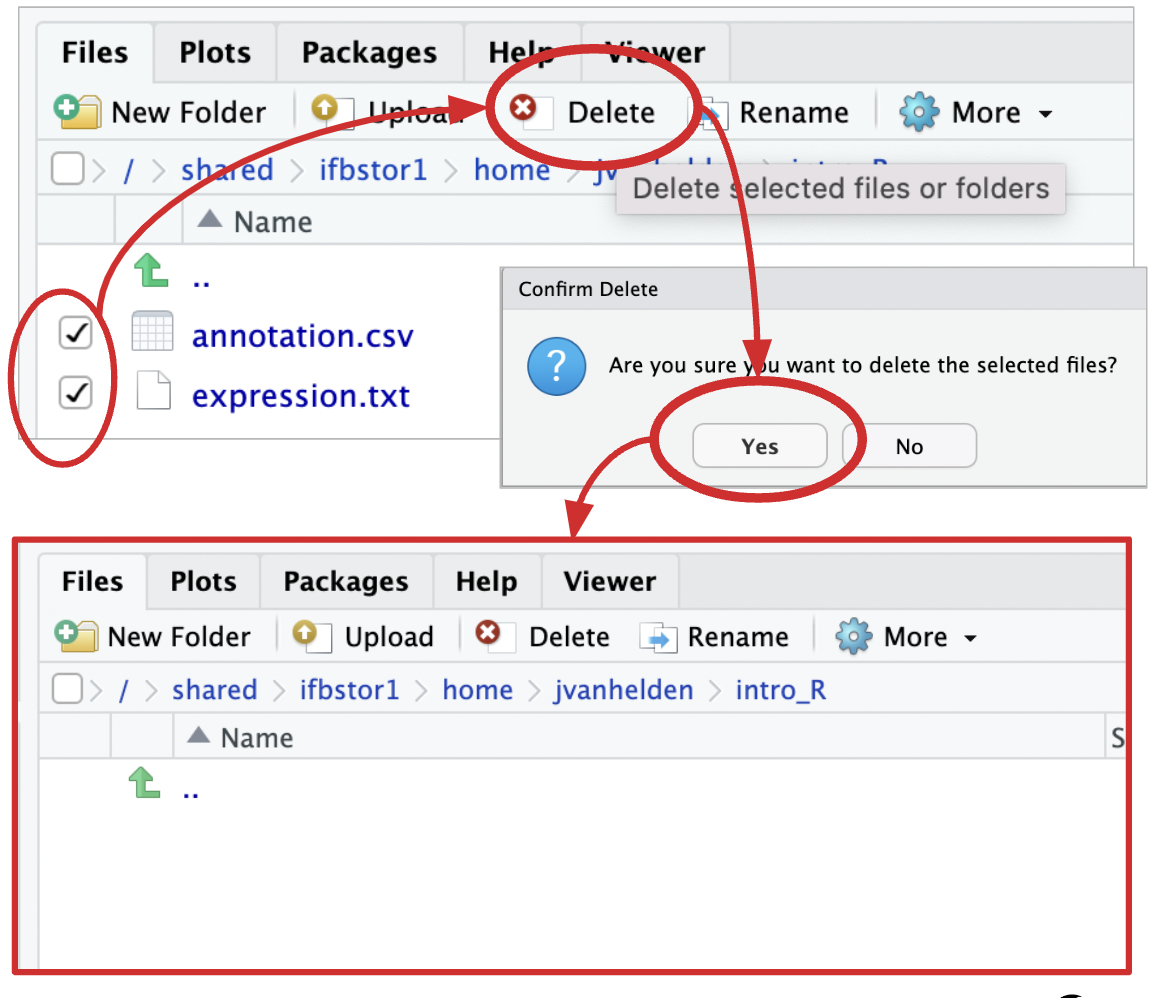
\includegraphics{images/delete.png}

Nous allons vous montrer une dernière façon de les téléverser.

\hypertarget{the-bash-geek-way-v3-directement-de-votre-home-du-cluster}{%
\section{The ``bash geek'' way (V3, directement de votre home du cluster)}\label{the-bash-geek-way-v3-directement-de-votre-home-du-cluster}}

Objectif

Dans le terminal du cluster, téléchargez et enregistrez dans votre home les fichiers de données:
- expression.txt: données d'expressions pour 4 échantillons
- annotation.csv: informations sur les gènes (id, name, chr, start, stop)

Ouvrez un connection ssh

\begin{Shaded}
\begin{Highlighting}[]
\FunctionTok{ssh}\NormalTok{ [votre\_login]@core.cluster.france{-}bioinformatique.fr}
\end{Highlighting}
\end{Shaded}

Où suis-je ?

\begin{Shaded}
\begin{Highlighting}[]
\BuiltInTok{pwd}
\end{Highlighting}
\end{Shaded}

\begin{verbatim}
## /shared/ifbstor1/projects/form_2022_32/EBAII_IntroR
\end{verbatim}

Créez un répertoire ``intro\_R''

\begin{Shaded}
\begin{Highlighting}[]
\FunctionTok{mkdir} \AttributeTok{{-}p}\NormalTok{ /shared/ifbstor1/projects/form\_2022\_32/EBAII\_IntroR/intro\_R}
\end{Highlighting}
\end{Shaded}

Déplacez-vous dans votre dossier

\begin{Shaded}
\begin{Highlighting}[]
\BuiltInTok{cd}\NormalTok{ /shared/ifbstor1/projects/form\_2022\_32/EBAII\_IntroR/intro\_R}
\end{Highlighting}
\end{Shaded}

Où suis-je maintenant ?

\begin{Shaded}
\begin{Highlighting}[]
\BuiltInTok{pwd}
\end{Highlighting}
\end{Shaded}

\begin{verbatim}
## /shared/ifbstor1/projects/form_2022_32/EBAII_IntroR
\end{verbatim}

Téléchargez les données

\begin{Shaded}
\begin{Highlighting}[]
\FunctionTok{wget}\NormalTok{ https://raw.githubusercontent.com/IFB{-}ElixirFr/EBAII/master/2022/ebaiin1/intro\_R/expression.txt }\AttributeTok{{-}{-}output{-}document}\OperatorTok{=}\NormalTok{expression.txt}
\end{Highlighting}
\end{Shaded}

\begin{verbatim}
## --2022-11-15 17:29:37--  https://raw.githubusercontent.com/IFB-ElixirFr/EBAII/master/2022/ebaiin1/intro_R/expression.txt
## Resolving raw.githubusercontent.com (raw.githubusercontent.com)... 185.199.111.133, 185.199.108.133, 185.199.110.133, ...
## Connecting to raw.githubusercontent.com (raw.githubusercontent.com)|185.199.111.133|:443... connected.
## HTTP request sent, awaiting response... 200 OK
## Length: 1747 (1.7K) [text/plain]
## Saving to: ‘expression.txt’
## 
##      0K .                                                     100% 18.3M=0s
## 
## 2022-11-15 17:29:37 (18.3 MB/s) - ‘expression.txt’ saved [1747/1747]
\end{verbatim}

\begin{Shaded}
\begin{Highlighting}[]
\FunctionTok{wget}\NormalTok{ https://raw.githubusercontent.com/IFB{-}ElixirFr/EBAII/master/2022/ebaiin1/intro\_R/annotation.csv }\AttributeTok{{-}O}\NormalTok{ annotation.csv}
\end{Highlighting}
\end{Shaded}

\begin{verbatim}
## --2022-11-15 17:29:37--  https://raw.githubusercontent.com/IFB-ElixirFr/EBAII/master/2022/ebaiin1/intro_R/annotation.csv
## Resolving raw.githubusercontent.com (raw.githubusercontent.com)... 185.199.111.133, 185.199.110.133, 185.199.109.133, ...
## Connecting to raw.githubusercontent.com (raw.githubusercontent.com)|185.199.111.133|:443... connected.
## HTTP request sent, awaiting response... 200 OK
## Length: 2326 (2.3K) [text/plain]
## Saving to: ‘annotation.csv’
## 
##      0K ..                                                    100% 26.2M=0s
## 
## 2022-11-15 17:29:37 (26.2 MB/s) - ‘annotation.csv’ saved [2326/2326]
\end{verbatim}

Qu'y a-t-il ici ?

\begin{Shaded}
\begin{Highlighting}[]
\FunctionTok{ls} \AttributeTok{{-}l}
\end{Highlighting}
\end{Shaded}

\begin{verbatim}
## total 316
## -rw-r--r--+ 1 tdenecker tdenecker   1843 Nov 15 09:19 01-intro.Rmd
## -rw-r--r--+ 1 tdenecker tdenecker    996 Nov 15 09:40 02-how.Rmd
## -rw-r--r--+ 1 tdenecker tdenecker   1478 Nov 15 09:48 03-firstSteps.Rmd
## -rw-r--r--+ 1 tdenecker tdenecker   5467 Nov 15 10:30 04-uploadData.Rmd
## -rw-r--r--+ 1 tdenecker tdenecker   1790 Nov 15 10:46 05-readData.Rmd
## -rw-r--r--+ 1 tdenecker tdenecker   1419 Nov 15 11:57 06-manipulate.Rmd
## -rw-r-----+ 1 tdenecker tdenecker   1882 Nov 15 12:20 07-plots.Rmd
## -rw-r-----+ 1 tdenecker tdenecker   2490 Nov 15 12:38 08-analyseDiff.Rmd
## -rw-r-----+ 1 tdenecker tdenecker   1490 Nov 15 15:51 09-integration.Rmd
## -rw-r-----+ 1 tdenecker tdenecker   1422 Nov 15 17:19 10-visu.Rmd
## -rw-r-----+ 1 tdenecker tdenecker   1128 Nov 15 12:35 11-conclusion.Rmd
## -rw-r--r--+ 1 tdenecker tdenecker     54 Nov 14 21:51 12-references.Rmd
## -rw-rw----+ 1 tdenecker tdenecker   2326 Nov 15 17:29 annotation.csv
## -rw-r--r--+ 1 tdenecker tdenecker    267 Nov 14 21:51 book.bib
## drwxrwx---+ 2 tdenecker tdenecker   4096 Nov 15 17:29 _bookdown_files
## -rw-r--r--+ 1 tdenecker tdenecker    113 Nov 15 16:00 _bookdown.yml
## drwxrwx---+ 5 tdenecker tdenecker  12288 Nov 15 17:29 docs
## -rw-rw----+ 1 tdenecker tdenecker    247 Nov 15 15:48 EBAII_IntroR.Rproj
## -rw-rw----+ 1 tdenecker tdenecker   1747 Nov 15 17:29 expression.txt
## -rw-rw----+ 1 tdenecker tdenecker    244 Nov 15 17:29 exprs_chr8.txt
## drwxrwx---+ 2 tdenecker tdenecker   4096 Nov 15 12:35 images
## -rw-r--r--+ 1 tdenecker tdenecker   1460 Nov 15 17:29 index.Rmd
## drwxrwx---+ 2 tdenecker tdenecker   4096 Nov 15 10:25 intro_R
## -rw-rw----+ 1 tdenecker tdenecker   1551 Nov 14 21:50 LICENSE
## drwxrwx---+ 4 tdenecker tdenecker   4096 Nov 15 17:29 _main_files
## -rw-rw----+ 1 tdenecker tdenecker  37392 Nov 15 17:28 _main.log
## -rw-rw----+ 1 tdenecker tdenecker  13209 Nov 15 17:28 _main.pdf
## -rw-r--r--+ 1 tdenecker tdenecker  23395 Nov 15 17:29 _main.Rmd
## -rw-rw----+ 1 tdenecker tdenecker 102254 Nov 15 17:28 _main.tex
## -rw-r--r--+ 1 tdenecker tdenecker    500 Nov 14 21:52 _output.yml
## -rw-rw----+ 1 tdenecker tdenecker   2655 Nov 15 17:29 packages.bib
## -rw-r--r--+ 1 tdenecker tdenecker     22 Nov 14 21:51 preamble.tex
## -rw-r--r--+ 1 tdenecker tdenecker    311 Nov 15 09:29 README.md
## -rw-r--r--+ 1 tdenecker tdenecker    172 Nov 14 21:51 style.css
\end{verbatim}

A quoi ressemblent ces fichiers ?

\begin{Shaded}
\begin{Highlighting}[]
\FunctionTok{head}\NormalTok{ expression.txt}
\end{Highlighting}
\end{Shaded}

\begin{verbatim}
## id   WT1 WT2 KO1 KO2
## ENSG00000034510  235960  94264   202381  91336
## ENSG00000064201  116 71  64  56
## ENSG00000065717  118 174 124 182
## ENSG00000099958  450 655 301 472
## ENSG00000104164  4736    5019    4845    4934
## ENSG00000104783  9002    8623    7720    7142
## ENSG00000105229  1295    2744    1113    2887
## ENSG00000105723  3353    7449    3589    7202
## ENSG00000116199  2044    4525    2604    4902
\end{verbatim}

\begin{Shaded}
\begin{Highlighting}[]
\FunctionTok{head}\NormalTok{ annotation.csv}
\end{Highlighting}
\end{Shaded}

\begin{verbatim}
## id;name;chr;start;stop;strand
## ENSG00000225630;MTND2P28;1;629640;630683;+
## ENSG00000134198;TSPAN2;1;115048011;115089500;-
## ENSG00000116199;FAM20B;1;179025804;179076562;+
## ENSG00000119285;HEATR1;1;236549005;236604504;-
## ENSG00000034510;TMSB10;2;84905625;84906675;+
## ENSG00000198586;TLK1;2;170990823;171231314;-
## ENSG00000157036;EXOG;3;38496127;38542161;+
## ENSG00000157869;RAB28;4;13361354;13484365;-
## ENSG00000250202;RP11-397E7.2;4;86876338;86876652;+
\end{verbatim}

\hypertarget{actualisation-du-dossier}{%
\section{Actualisation du dossier}\label{actualisation-du-dossier}}

Dans certains cas, il faut actualiser le contenu du dossier pour pouvoir voir le nouveau sous-dossier.
Vérifiez ensuite si \texttt{intro\_R} apparaît bien dans le contenu de votre dossier principal.

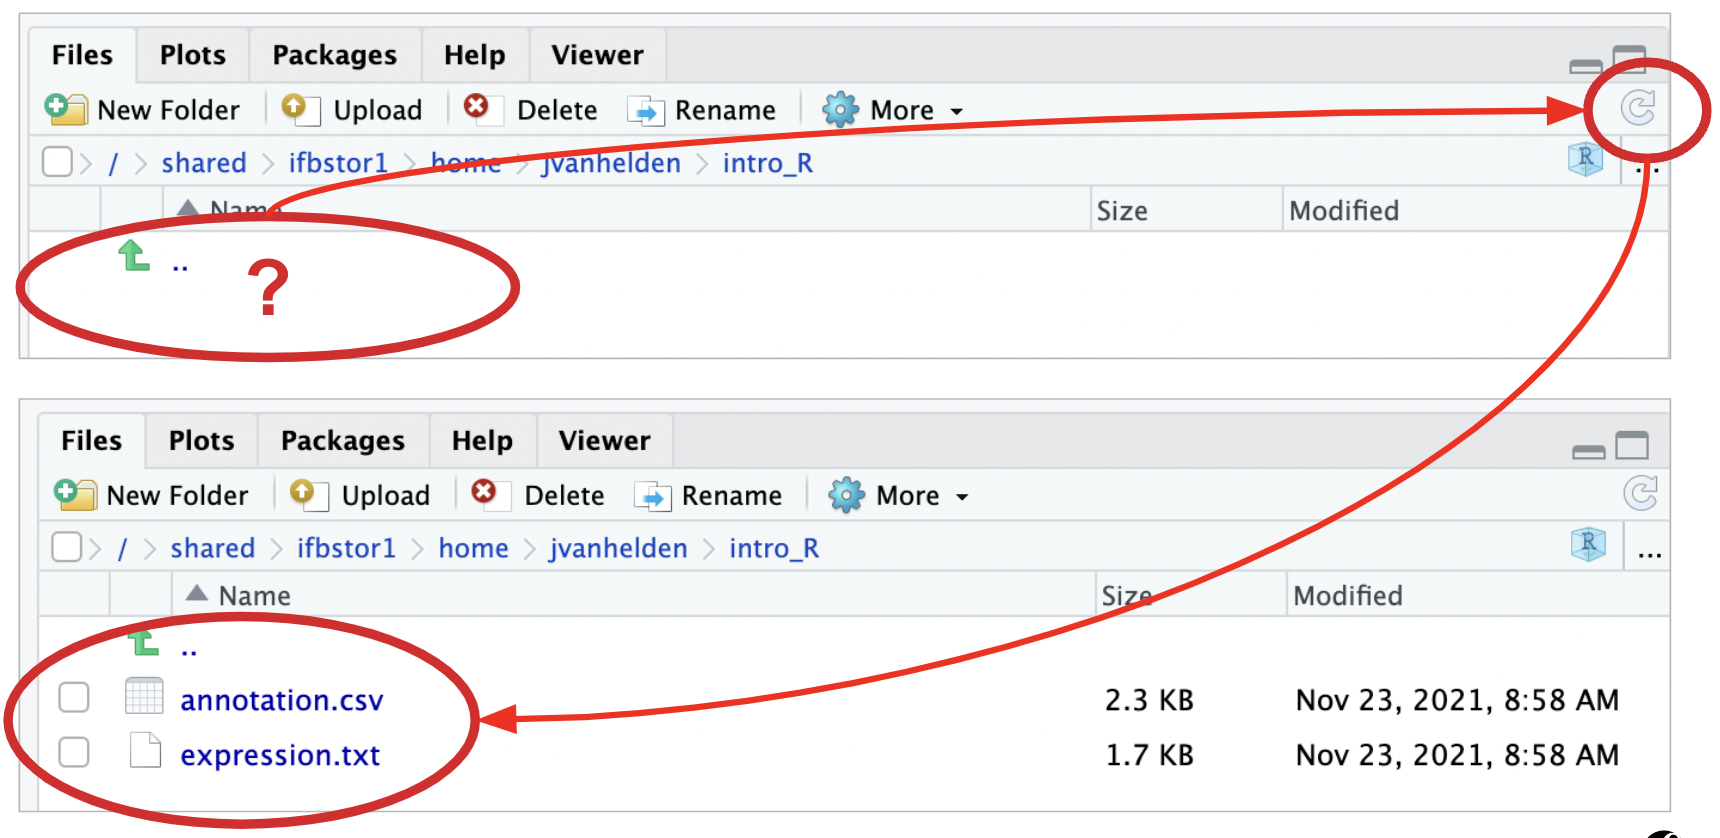
\includegraphics{images/actualiser.png}

\hypertarget{lecture-des-donnuxe9es}{%
\chapter{Lecture des données}\label{lecture-des-donnuxe9es}}

\hypertarget{chargement-des-donnuxe9es-dans-la-muxe9moire-de-r}{%
\section{Chargement des données (dans la mémoire de R)}\label{chargement-des-donnuxe9es-dans-la-muxe9moire-de-r}}

Charger le contenu du fichier ``expression.txt'' dans une variable nommée ``exprs''.

\begin{Shaded}
\begin{Highlighting}[]
\NormalTok{exprs }\OtherTok{\textless{}{-}} \FunctionTok{read.table}\NormalTok{(}\AttributeTok{file =} \StringTok{"expression.txt"}\NormalTok{, }\AttributeTok{header =} \ConstantTok{TRUE}\NormalTok{, }\AttributeTok{sep =} \StringTok{"}\SpecialCharTok{\textbackslash{}t}\StringTok{"}\NormalTok{)}
\end{Highlighting}
\end{Shaded}

Accéder à l'aide d'une fonction

\begin{Shaded}
\begin{Highlighting}[]
\FunctionTok{help}\NormalTok{(read.table)}
\end{Highlighting}
\end{Shaded}

Notation alternative

\begin{Shaded}
\begin{Highlighting}[]
\NormalTok{?read.table}
\end{Highlighting}
\end{Shaded}

Recherche interactive sous RStudio
- Sélectionner l'onglet ``Help'' du panneau inférieur droit.
- Taper ``read.table'' dans la boîte de recherche.

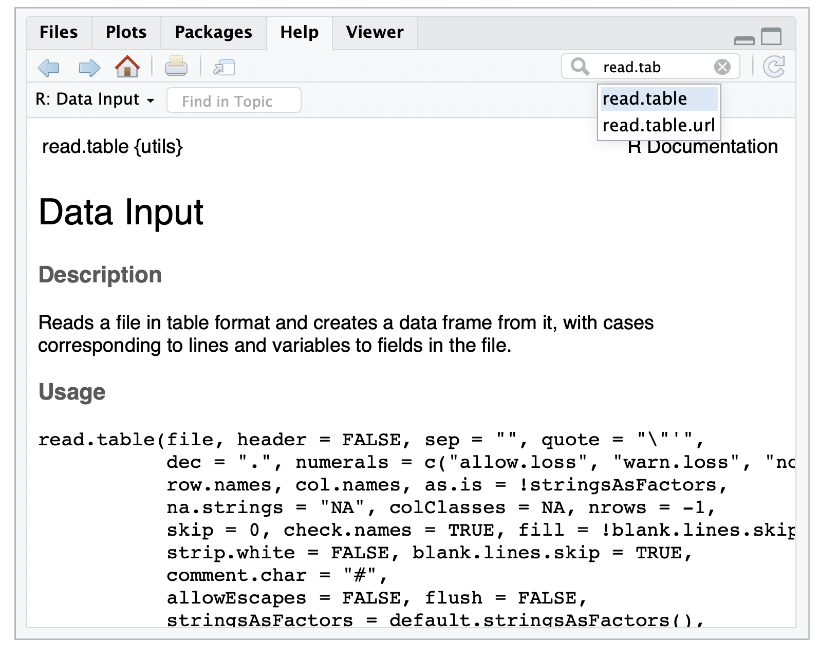
\includegraphics{images/help.png}

Sinon, une approche plus simple et plus pratique :
- demande à Google ``Comment lire une table en R ?''
- adapte l'exemple

\hypertarget{affichage-de-lobjet-exprs}{%
\section{Affichage de l'objet ``exprs''}\label{affichage-de-lobjet-exprs}}

Imprimer toutes les valeurs.

\begin{Shaded}
\begin{Highlighting}[]
\FunctionTok{print}\NormalTok{(exprs)}
\end{Highlighting}
\end{Shaded}

\begin{verbatim}
##                 id    WT1   WT2    KO1   KO2
## 1  ENSG00000034510 235960 94264 202381 91336
## 2  ENSG00000064201    116    71     64    56
## 3  ENSG00000065717    118   174    124   182
## 4  ENSG00000099958    450   655    301   472
## 5  ENSG00000104164   4736  5019   4845  4934
## 6  ENSG00000104783   9002  8623   7720  7142
## 7  ENSG00000105229   1295  2744   1113  2887
## 8  ENSG00000105723   3353  7449   3589  7202
## 9  ENSG00000116199   2044  4525   2604  4902
## 10 ENSG00000118939   7022  2526   6269  3068
## 11 ENSG00000119285  15783 17359  18591 20077
## 12 ENSG00000121680   3133  2775   2045  2796
## 13 ENSG00000125384   1380  3079    869  2419
## 14 ENSG00000129562  12089  7958  10708  7683
## 15 ENSG00000129932   1744  2247   1513  3104
## 16 ENSG00000134198    122    66     44    16
## 17 ENSG00000135452    635   427    662   291
## 18 ENSG00000140416     83   246    136   267
## 19 ENSG00000147274  16013 17642  15055 18804
## 20 ENSG00000148090    552  1062    615  1082
## 21 ENSG00000148248  62324 33973  56862 37710
## 22 ENSG00000157036   1225  1475   1275  1373
## 23 ENSG00000157869   1201  1034   1025   858
## 24 ENSG00000159433     31   788     30   675
## 25 ENSG00000161692    695  1825    746  1851
## 26 ENSG00000167005  26866 23111  24888 22661
## 27 ENSG00000168517    273   112    190    77
## 28 ENSG00000169570    202   181    207   209
## 29 ENSG00000172216   3515  1981   3204  3174
## 30 ENSG00000175221   1988  4788   2115  5306
## 31 ENSG00000183161   2238   974   2089   996
## 32 ENSG00000185324   1236  2163   1048  2024
## 33 ENSG00000188985   3415  1703   3587  2096
## 34 ENSG00000196867    209   189    293   192
## 35 ENSG00000197081  14741 36309  14941 29645
## 36 ENSG00000198586   1216  4545   1660  3932
## 37 ENSG00000214121   4044  2575   3019  2506
## 38 ENSG00000225630   1405  8135   1569  7866
## 39 ENSG00000226742    158    94    153   178
## 40 ENSG00000238241     90    43    122   143
## 41 ENSG00000248751    518   718    411   597
## 42 ENSG00000250202    261   163    177   191
## 43 ENSG00000251106     94   114     63    86
## 44 ENSG00000253991     77    78    134    92
## 45 ENSG00000254470   3025  3707   2558  4066
## 46 ENSG00000262814  15470 11450  11656 13821
## 47 ENSG00000267228   3801  2465   2787  2301
## 48 ENSG00000267699   1488  1086   1374   939
## 49 ENSG00000269293    424   162    310   120
## 50 ENSG00000279329     55    76     58    70
\end{verbatim}

Affichage des premières lignes de l'objet

\begin{Shaded}
\begin{Highlighting}[]
\FunctionTok{head}\NormalTok{(exprs)}
\end{Highlighting}
\end{Shaded}

\begin{verbatim}
##                id    WT1   WT2    KO1   KO2
## 1 ENSG00000034510 235960 94264 202381 91336
## 2 ENSG00000064201    116    71     64    56
## 3 ENSG00000065717    118   174    124   182
## 4 ENSG00000099958    450   655    301   472
## 5 ENSG00000104164   4736  5019   4845  4934
## 6 ENSG00000104783   9002  8623   7720  7142
\end{verbatim}

Affichage des dernières lignes de l'objet

\begin{Shaded}
\begin{Highlighting}[]
\FunctionTok{tail}\NormalTok{(exprs)}
\end{Highlighting}
\end{Shaded}

\begin{verbatim}
##                 id   WT1   WT2   KO1   KO2
## 45 ENSG00000254470  3025  3707  2558  4066
## 46 ENSG00000262814 15470 11450 11656 13821
## 47 ENSG00000267228  3801  2465  2787  2301
## 48 ENSG00000267699  1488  1086  1374   939
## 49 ENSG00000269293   424   162   310   120
## 50 ENSG00000279329    55    76    58    70
\end{verbatim}

Un peu plus de lignes

\begin{Shaded}
\begin{Highlighting}[]
\FunctionTok{head}\NormalTok{(exprs, }\AttributeTok{n =} \DecValTok{15}\NormalTok{)}
\end{Highlighting}
\end{Shaded}

\begin{verbatim}
##                 id    WT1   WT2    KO1   KO2
## 1  ENSG00000034510 235960 94264 202381 91336
## 2  ENSG00000064201    116    71     64    56
## 3  ENSG00000065717    118   174    124   182
## 4  ENSG00000099958    450   655    301   472
## 5  ENSG00000104164   4736  5019   4845  4934
## 6  ENSG00000104783   9002  8623   7720  7142
## 7  ENSG00000105229   1295  2744   1113  2887
## 8  ENSG00000105723   3353  7449   3589  7202
## 9  ENSG00000116199   2044  4525   2604  4902
## 10 ENSG00000118939   7022  2526   6269  3068
## 11 ENSG00000119285  15783 17359  18591 20077
## 12 ENSG00000121680   3133  2775   2045  2796
## 13 ENSG00000125384   1380  3079    869  2419
## 14 ENSG00000129562  12089  7958  10708  7683
## 15 ENSG00000129932   1744  2247   1513  3104
\end{verbatim}

Explorer le tableau dans un panneau de visualisation

\begin{Shaded}
\begin{Highlighting}[]
\FunctionTok{View}\NormalTok{(exprs)}
\end{Highlighting}
\end{Shaded}

\textbf{Note}: vous pouvez cliquer sur une en-tête de colonne pour trier les données

Explorer le tableau avec le package \href{https://rstudio.github.io/DT/}{DT}

\begin{Shaded}
\begin{Highlighting}[]
\FunctionTok{library}\NormalTok{(DT)}
\FunctionTok{datatable}\NormalTok{(exprs)}
\end{Highlighting}
\end{Shaded}

\begin{verbatim}
## PhantomJS not found. You can install it with webshot::install_phantomjs(). If it is installed, please make sure the phantomjs executable can be found via the PATH variable.
\end{verbatim}

\hypertarget{caractuxe9ristiques-dun-tableau-de-donnuxe9es}{%
\section{Caractéristiques d'un tableau de données}\label{caractuxe9ristiques-dun-tableau-de-donnuxe9es}}

\hypertarget{dimensions}{%
\subsection{Dimensions}\label{dimensions}}

Nombre de colonnes

\begin{Shaded}
\begin{Highlighting}[]
\FunctionTok{ncol}\NormalTok{(exprs)}
\end{Highlighting}
\end{Shaded}

\begin{verbatim}
## [1] 5
\end{verbatim}

Nombre de lignes

\begin{Shaded}
\begin{Highlighting}[]
\FunctionTok{nrow}\NormalTok{(exprs) }
\end{Highlighting}
\end{Shaded}

\begin{verbatim}
## [1] 50
\end{verbatim}

Dimensions

\begin{Shaded}
\begin{Highlighting}[]
\FunctionTok{dim}\NormalTok{(exprs)}
\end{Highlighting}
\end{Shaded}

\begin{verbatim}
## [1] 50  5
\end{verbatim}

\hypertarget{noms-des-colonnes-et-des-lignes}{%
\subsection{Noms des colonnes et des lignes}\label{noms-des-colonnes-et-des-lignes}}

Noms des colonnes

\begin{Shaded}
\begin{Highlighting}[]
\FunctionTok{colnames}\NormalTok{(exprs)}
\end{Highlighting}
\end{Shaded}

\begin{verbatim}
## [1] "id"  "WT1" "WT2" "KO1" "KO2"
\end{verbatim}

Idem

\begin{Shaded}
\begin{Highlighting}[]
\FunctionTok{names}\NormalTok{(exprs) }
\end{Highlighting}
\end{Shaded}

\begin{verbatim}
## [1] "id"  "WT1" "WT2" "KO1" "KO2"
\end{verbatim}

Noms des lignes

\begin{Shaded}
\begin{Highlighting}[]
\FunctionTok{rownames}\NormalTok{(exprs)}
\end{Highlighting}
\end{Shaded}

\begin{verbatim}
##  [1] "1"  "2"  "3"  "4"  "5"  "6"  "7"  "8"  "9"  "10" "11" "12" "13" "14" "15"
## [16] "16" "17" "18" "19" "20" "21" "22" "23" "24" "25" "26" "27" "28" "29" "30"
## [31] "31" "32" "33" "34" "35" "36" "37" "38" "39" "40" "41" "42" "43" "44" "45"
## [46] "46" "47" "48" "49" "50"
\end{verbatim}

\hypertarget{ruxe9sumuxe9-rapide-des-donnuxe9es-par-colonne}{%
\subsection{Résumé rapide des données par colonne}\label{ruxe9sumuxe9-rapide-des-donnuxe9es-par-colonne}}

Statistiques par colonne

\begin{Shaded}
\begin{Highlighting}[]
\FunctionTok{summary}\NormalTok{(exprs)}
\end{Highlighting}
\end{Shaded}

\begin{verbatim}
##       id                 WT1              WT2               KO1          
##  Length:50          Min.   :    31   Min.   :   43.0   Min.   :    30.0  
##  Class :character   1st Qu.:   264   1st Qu.:  203.2   1st Qu.:   228.5  
##  Mode  :character   Median :  1338   Median : 1903.0   Median :  1324.5  
##                     Mean   :  9358   Mean   : 6498.6   Mean   :  8356.0  
##                     3rd Qu.:  3730   3rd Qu.: 4727.2   3rd Qu.:  3491.2  
##                     Max.   :235960   Max.   :94264.0   Max.   :202381.0  
##       KO2         
##  Min.   :   16.0  
##  1st Qu.:  223.5  
##  Median : 2060.0  
##  Mean   : 6489.5  
##  3rd Qu.: 4926.0  
##  Max.   :91336.0
\end{verbatim}

Structure de la variable

\begin{Shaded}
\begin{Highlighting}[]
\FunctionTok{str}\NormalTok{(exprs)}
\end{Highlighting}
\end{Shaded}

\begin{verbatim}
## 'data.frame':    50 obs. of  5 variables:
##  $ id : chr  "ENSG00000034510" "ENSG00000064201" "ENSG00000065717" "ENSG00000099958" ...
##  $ WT1: int  235960 116 118 450 4736 9002 1295 3353 2044 7022 ...
##  $ WT2: int  94264 71 174 655 5019 8623 2744 7449 4525 2526 ...
##  $ KO1: int  202381 64 124 301 4845 7720 1113 3589 2604 6269 ...
##  $ KO2: int  91336 56 182 472 4934 7142 2887 7202 4902 3068 ...
\end{verbatim}

Même résultat que dans le panneau ``Environment''

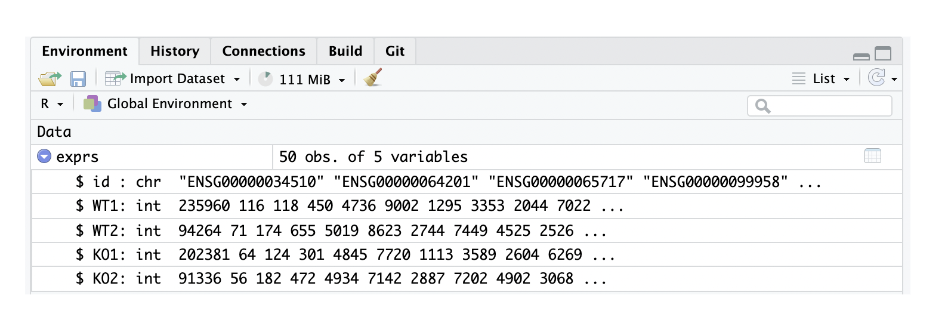
\includegraphics{images/envExpr.png}

\hypertarget{manipuler-les-donnuxe9es-dans-r}{%
\chapter{Manipuler les données dans R}\label{manipuler-les-donnuxe9es-dans-r}}

\hypertarget{suxe9lection-de-colonnes-dun-tableau}{%
\section{Sélection de colonnes d'un tableau}\label{suxe9lection-de-colonnes-dun-tableau}}

Afficher les noms des colonnes

\begin{Shaded}
\begin{Highlighting}[]
\FunctionTok{colnames}\NormalTok{(exprs)}
\end{Highlighting}
\end{Shaded}

\begin{verbatim}
## [1] "id"  "WT1" "WT2" "KO1" "KO2"
\end{verbatim}

Valeurs stockées dans la colonne nommée ``WT1''

\begin{Shaded}
\begin{Highlighting}[]
\NormalTok{exprs}\SpecialCharTok{$}\NormalTok{WT1}
\end{Highlighting}
\end{Shaded}

\begin{verbatim}
##  [1] 235960    116    118    450   4736   9002   1295   3353   2044   7022
## [11]  15783   3133   1380  12089   1744    122    635     83  16013    552
## [21]  62324   1225   1201     31    695  26866    273    202   3515   1988
## [31]   2238   1236   3415    209  14741   1216   4044   1405    158     90
## [41]    518    261     94     77   3025  15470   3801   1488    424     55
\end{verbatim}

Notation alternative

\begin{Shaded}
\begin{Highlighting}[]
\NormalTok{exprs[ , }\StringTok{"WT1"}\NormalTok{]}
\end{Highlighting}
\end{Shaded}

\begin{verbatim}
##  [1] 235960    116    118    450   4736   9002   1295   3353   2044   7022
## [11]  15783   3133   1380  12089   1744    122    635     83  16013    552
## [21]  62324   1225   1201     31    695  26866    273    202   3515   1988
## [31]   2238   1236   3415    209  14741   1216   4044   1405    158     90
## [41]    518    261     94     77   3025  15470   3801   1488    424     55
\end{verbatim}

Sélection de plusieurs colonnes.

\begin{Shaded}
\begin{Highlighting}[]
\NormalTok{exprs[ , }\FunctionTok{c}\NormalTok{(}\StringTok{"WT1"}\NormalTok{, }\StringTok{"WT2"}\NormalTok{)]}
\end{Highlighting}
\end{Shaded}

\begin{verbatim}
##       WT1   WT2
## 1  235960 94264
## 2     116    71
## 3     118   174
## 4     450   655
## 5    4736  5019
## 6    9002  8623
## 7    1295  2744
## 8    3353  7449
## 9    2044  4525
## 10   7022  2526
## 11  15783 17359
## 12   3133  2775
## 13   1380  3079
## 14  12089  7958
## 15   1744  2247
## 16    122    66
## 17    635   427
## 18     83   246
## 19  16013 17642
## 20    552  1062
## 21  62324 33973
## 22   1225  1475
## 23   1201  1034
## 24     31   788
## 25    695  1825
## 26  26866 23111
## 27    273   112
## 28    202   181
## 29   3515  1981
## 30   1988  4788
## 31   2238   974
## 32   1236  2163
## 33   3415  1703
## 34    209   189
## 35  14741 36309
## 36   1216  4545
## 37   4044  2575
## 38   1405  8135
## 39    158    94
## 40     90    43
## 41    518   718
## 42    261   163
## 43     94   114
## 44     77    78
## 45   3025  3707
## 46  15470 11450
## 47   3801  2465
## 48   1488  1086
## 49    424   162
## 50     55    76
\end{verbatim}

Sélection de colonnes par leur indice

\begin{Shaded}
\begin{Highlighting}[]
\NormalTok{exprs[ , }\DecValTok{2}\NormalTok{]}
\end{Highlighting}
\end{Shaded}

\begin{verbatim}
##  [1] 235960    116    118    450   4736   9002   1295   3353   2044   7022
## [11]  15783   3133   1380  12089   1744    122    635     83  16013    552
## [21]  62324   1225   1201     31    695  26866    273    202   3515   1988
## [31]   2238   1236   3415    209  14741   1216   4044   1405    158     90
## [41]    518    261     94     77   3025  15470   3801   1488    424     55
\end{verbatim}

\begin{Shaded}
\begin{Highlighting}[]
\NormalTok{exprs[ , }\FunctionTok{c}\NormalTok{( }\DecValTok{3}\NormalTok{, }\DecValTok{2}\NormalTok{)]}
\end{Highlighting}
\end{Shaded}

\begin{verbatim}
##      WT2    WT1
## 1  94264 235960
## 2     71    116
## 3    174    118
## 4    655    450
## 5   5019   4736
## 6   8623   9002
## 7   2744   1295
## 8   7449   3353
## 9   4525   2044
## 10  2526   7022
## 11 17359  15783
## 12  2775   3133
## 13  3079   1380
## 14  7958  12089
## 15  2247   1744
## 16    66    122
## 17   427    635
## 18   246     83
## 19 17642  16013
## 20  1062    552
## 21 33973  62324
## 22  1475   1225
## 23  1034   1201
## 24   788     31
## 25  1825    695
## 26 23111  26866
## 27   112    273
## 28   181    202
## 29  1981   3515
## 30  4788   1988
## 31   974   2238
## 32  2163   1236
## 33  1703   3415
## 34   189    209
## 35 36309  14741
## 36  4545   1216
## 37  2575   4044
## 38  8135   1405
## 39    94    158
## 40    43     90
## 41   718    518
## 42   163    261
## 43   114     94
## 44    78     77
## 45  3707   3025
## 46 11450  15470
## 47  2465   3801
## 48  1086   1488
## 49   162    424
## 50    76     55
\end{verbatim}

\hypertarget{suxe9lection-de-lignes-dun-tableau}{%
\section{Sélection de lignes d'un tableau}\label{suxe9lection-de-lignes-dun-tableau}}

Sélection des lignes 4 et 11 du tableau des expressions

\begin{Shaded}
\begin{Highlighting}[]
\NormalTok{exprs[}\FunctionTok{c}\NormalTok{(}\DecValTok{4}\NormalTok{, }\DecValTok{11}\NormalTok{), ]}
\end{Highlighting}
\end{Shaded}

\begin{verbatim}
##                 id   WT1   WT2   KO1   KO2
## 4  ENSG00000099958   450   655   301   472
## 11 ENSG00000119285 15783 17359 18591 20077
\end{verbatim}

Sélection des identifiants de deux gènes d'intérêt

\begin{Shaded}
\begin{Highlighting}[]
\NormalTok{my\_genes }\OtherTok{\textless{}{-}} \FunctionTok{c}\NormalTok{(}\StringTok{"ENSG00000253991"}\NormalTok{, }\StringTok{"ENSG00000099958"}\NormalTok{)}
\end{Highlighting}
\end{Shaded}

Vecteur booléen indiquant si chaque ID du tableau fait partie des gènes d'intérêt

\begin{Shaded}
\begin{Highlighting}[]
\NormalTok{exprs}\SpecialCharTok{$}\NormalTok{id }\SpecialCharTok{\%in\%}\NormalTok{ my\_genes}
\end{Highlighting}
\end{Shaded}

\begin{verbatim}
##  [1] FALSE FALSE FALSE  TRUE FALSE FALSE FALSE FALSE FALSE FALSE FALSE FALSE
## [13] FALSE FALSE FALSE FALSE FALSE FALSE FALSE FALSE FALSE FALSE FALSE FALSE
## [25] FALSE FALSE FALSE FALSE FALSE FALSE FALSE FALSE FALSE FALSE FALSE FALSE
## [37] FALSE FALSE FALSE FALSE FALSE FALSE FALSE  TRUE FALSE FALSE FALSE FALSE
## [49] FALSE FALSE
\end{verbatim}

Indices des lignes correspondant aux IDs des gènes d'intérêt

\begin{Shaded}
\begin{Highlighting}[]
\FunctionTok{which}\NormalTok{(exprs}\SpecialCharTok{$}\NormalTok{id }\SpecialCharTok{\%in\%}\NormalTok{ my\_genes)}
\end{Highlighting}
\end{Shaded}

\begin{verbatim}
## [1]  4 44
\end{verbatim}

Afficher les lignes correspondantes

\begin{Shaded}
\begin{Highlighting}[]
\NormalTok{exprs[}\FunctionTok{which}\NormalTok{(exprs}\SpecialCharTok{$}\NormalTok{id }\SpecialCharTok{\%in\%}\NormalTok{ my\_genes),   ]}
\end{Highlighting}
\end{Shaded}

\begin{verbatim}
##                 id WT1 WT2 KO1 KO2
## 4  ENSG00000099958 450 655 301 472
## 44 ENSG00000253991  77  78 134  92
\end{verbatim}

\hypertarget{formulation-plus-intuitive}{%
\section{formulation plus intuitive}\label{formulation-plus-intuitive}}

\begin{Shaded}
\begin{Highlighting}[]
\FunctionTok{subset}\NormalTok{(}\AttributeTok{x =}\NormalTok{ exprs, id }\SpecialCharTok{\%in\%}\NormalTok{ my\_genes)     }
\end{Highlighting}
\end{Shaded}

\begin{verbatim}
##                 id WT1 WT2 KO1 KO2
## 4  ENSG00000099958 450 655 301 472
## 44 ENSG00000253991  77  78 134  92
\end{verbatim}

Approche plus moderne, avec le package dplyr

\begin{Shaded}
\begin{Highlighting}[]
\DocumentationTok{\#\# charger la librairie dplyr}
\FunctionTok{library}\NormalTok{(dplyr)  }
\end{Highlighting}
\end{Shaded}

\begin{verbatim}
## 
## Attaching package: 'dplyr'
\end{verbatim}

\begin{verbatim}
## The following objects are masked from 'package:stats':
## 
##     filter, lag
\end{verbatim}

\begin{verbatim}
## The following objects are masked from 'package:base':
## 
##     intersect, setdiff, setequal, union
\end{verbatim}

\begin{Shaded}
\begin{Highlighting}[]
\DocumentationTok{\#\# envoyer le tableau exprs à la commande filter()}
\NormalTok{exprs }\SpecialCharTok{\%\textgreater{}\%} \FunctionTok{filter}\NormalTok{(id }\SpecialCharTok{\%in\%}\NormalTok{ my\_genes)  }
\end{Highlighting}
\end{Shaded}

\begin{verbatim}
##                id WT1 WT2 KO1 KO2
## 1 ENSG00000099958 450 655 301 472
## 2 ENSG00000253991  77  78 134  92
\end{verbatim}

\begin{Shaded}
\begin{Highlighting}[]
\DocumentationTok{\#\# plus avancé : enchaîner plusieurs commandes}
\NormalTok{exprs }\SpecialCharTok{\%\textgreater{}\%} 
  \FunctionTok{filter}\NormalTok{(id }\SpecialCharTok{\%in\%}\NormalTok{ my\_genes) }\SpecialCharTok{\%\textgreater{}\%} 
  \FunctionTok{mutate}\NormalTok{(}\AttributeTok{mean\_KO =}\NormalTok{ (KO1 }\SpecialCharTok{+}\NormalTok{ KO2)}\SpecialCharTok{/}\DecValTok{2}\NormalTok{)   }
\end{Highlighting}
\end{Shaded}

\begin{verbatim}
##                id WT1 WT2 KO1 KO2 mean_KO
## 1 ENSG00000099958 450 655 301 472   386.5
## 2 ENSG00000253991  77  78 134  92   113.0
\end{verbatim}

\hypertarget{visualisation-des-donnuxe9es}{%
\chapter{Visualisation des données}\label{visualisation-des-donnuxe9es}}

\hypertarget{histogrammes}{%
\section{Histogrammes}\label{histogrammes}}

\hypertarget{avec-r-de-base}{%
\subsection{Avec R de base}\label{avec-r-de-base}}

Histogramme des valeurs d'expression pour l'échantillon WT1

\begin{Shaded}
\begin{Highlighting}[]
\FunctionTok{hist}\NormalTok{(exprs}\SpecialCharTok{$}\NormalTok{WT1)}
\end{Highlighting}
\end{Shaded}

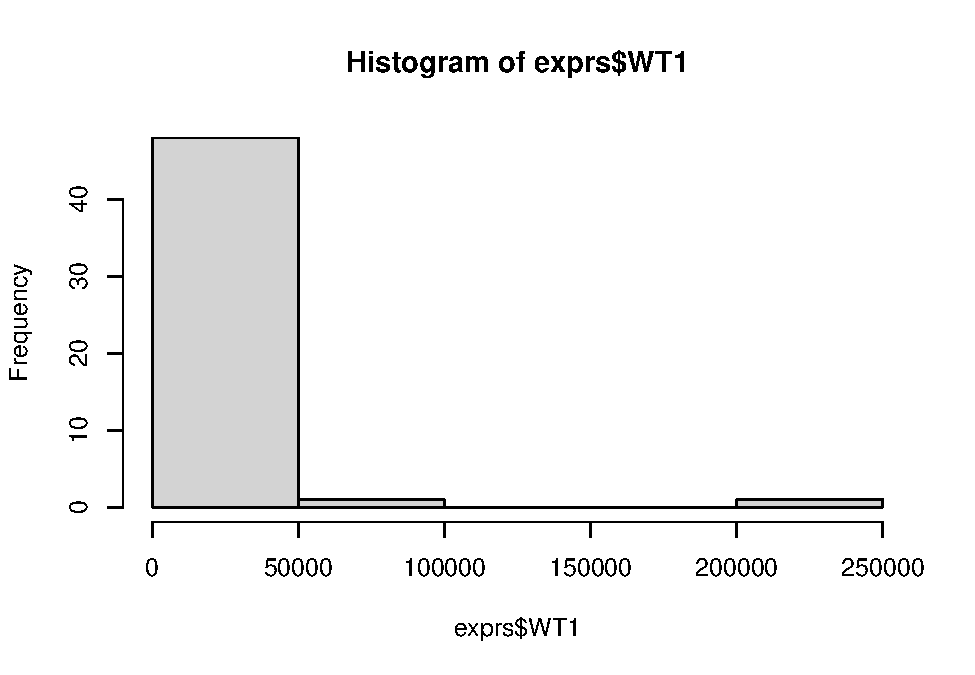
\includegraphics{_main_files/figure-latex/unnamed-chunk-72-1.pdf}

Histogramme du logarithme de ces valeurs

\begin{Shaded}
\begin{Highlighting}[]
\FunctionTok{hist}\NormalTok{(}\FunctionTok{log}\NormalTok{(exprs}\SpecialCharTok{$}\NormalTok{WT1))}
\end{Highlighting}
\end{Shaded}

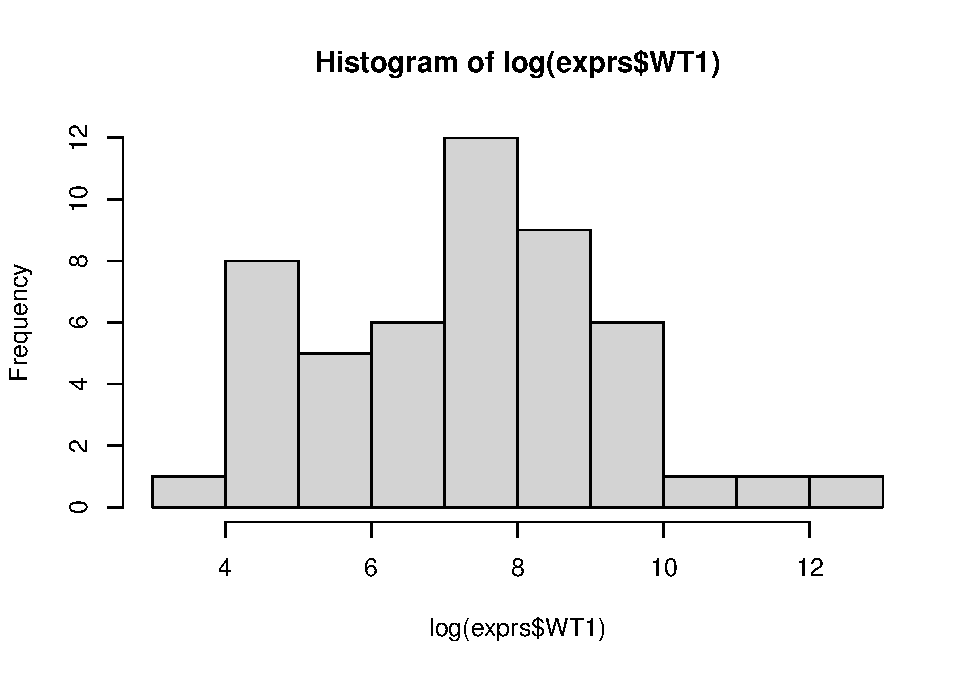
\includegraphics{_main_files/figure-latex/unnamed-chunk-73-1.pdf}

\begin{Shaded}
\begin{Highlighting}[]
\FunctionTok{hist}\NormalTok{(}\FunctionTok{log10}\NormalTok{(exprs}\SpecialCharTok{$}\NormalTok{WT1))}
\end{Highlighting}
\end{Shaded}

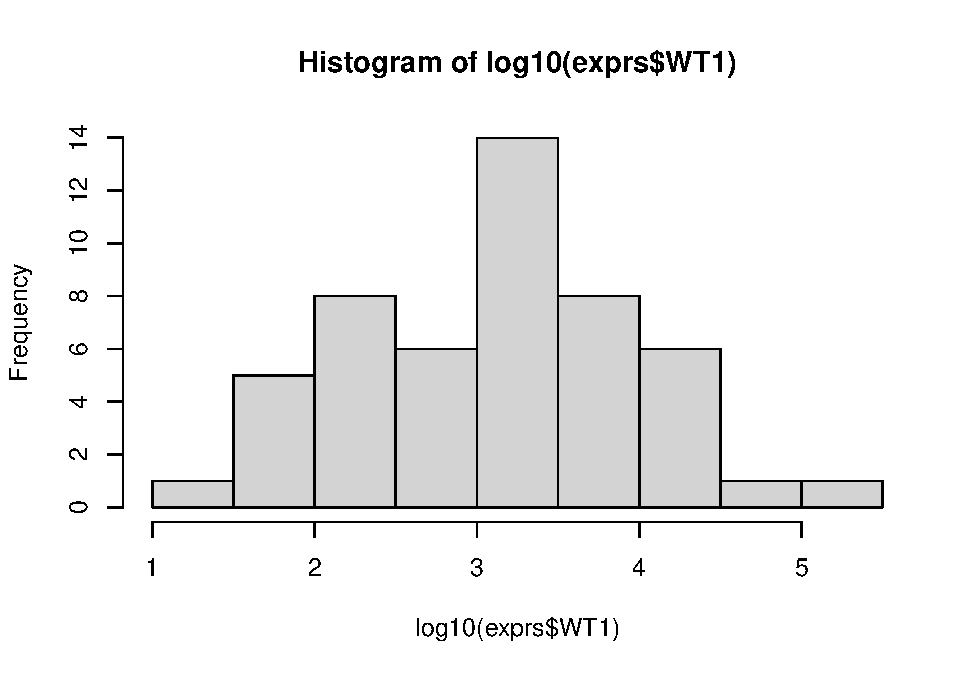
\includegraphics{_main_files/figure-latex/unnamed-chunk-74-1.pdf}

\begin{Shaded}
\begin{Highlighting}[]
\FunctionTok{hist}\NormalTok{(}\FunctionTok{log2}\NormalTok{(exprs}\SpecialCharTok{$}\NormalTok{WT1))}
\end{Highlighting}
\end{Shaded}

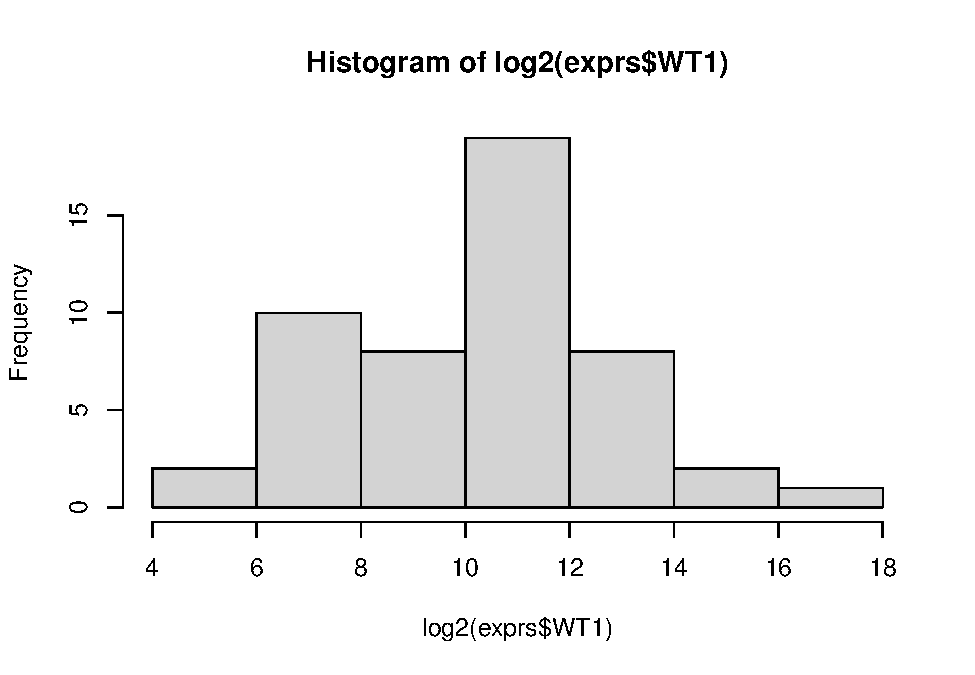
\includegraphics{_main_files/figure-latex/unnamed-chunk-75-1.pdf}

\hypertarget{avec-ggplot2}{%
\subsection{Avec ggplot2}\label{avec-ggplot2}}

\begin{Shaded}
\begin{Highlighting}[]
\FunctionTok{library}\NormalTok{(ggplot2)}
\end{Highlighting}
\end{Shaded}

\begin{verbatim}
## Warning: package 'ggplot2' was built under R version 4.1.3
\end{verbatim}

\begin{Shaded}
\begin{Highlighting}[]
\FunctionTok{ggplot}\NormalTok{(exprs, }\FunctionTok{aes}\NormalTok{(}\AttributeTok{x=}\NormalTok{WT1)) }\SpecialCharTok{+} \FunctionTok{geom\_histogram}\NormalTok{()}
\end{Highlighting}
\end{Shaded}

\begin{verbatim}
## `stat_bin()` using `bins = 30`. Pick better value with `binwidth`.
\end{verbatim}

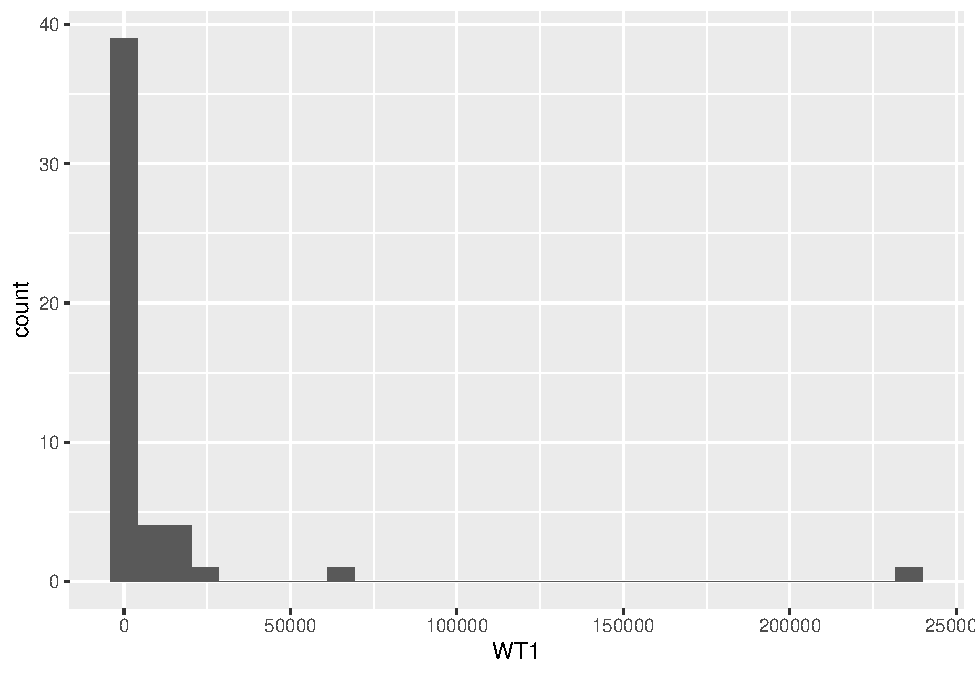
\includegraphics{_main_files/figure-latex/unnamed-chunk-76-1.pdf}

\hypertarget{bouxeetes-uxe0-moustaches-boxplots}{%
\section{Boîtes à moustaches (boxplots)}\label{bouxeetes-uxe0-moustaches-boxplots}}

\hypertarget{avec-r-de-base-1}{%
\subsection{Avec R de base}\label{avec-r-de-base-1}}

Boite à moustache des valeurs d'expression pour l'échantillon WT1

\begin{Shaded}
\begin{Highlighting}[]
\FunctionTok{boxplot}\NormalTok{(exprs}\SpecialCharTok{$}\NormalTok{WT1)}
\end{Highlighting}
\end{Shaded}

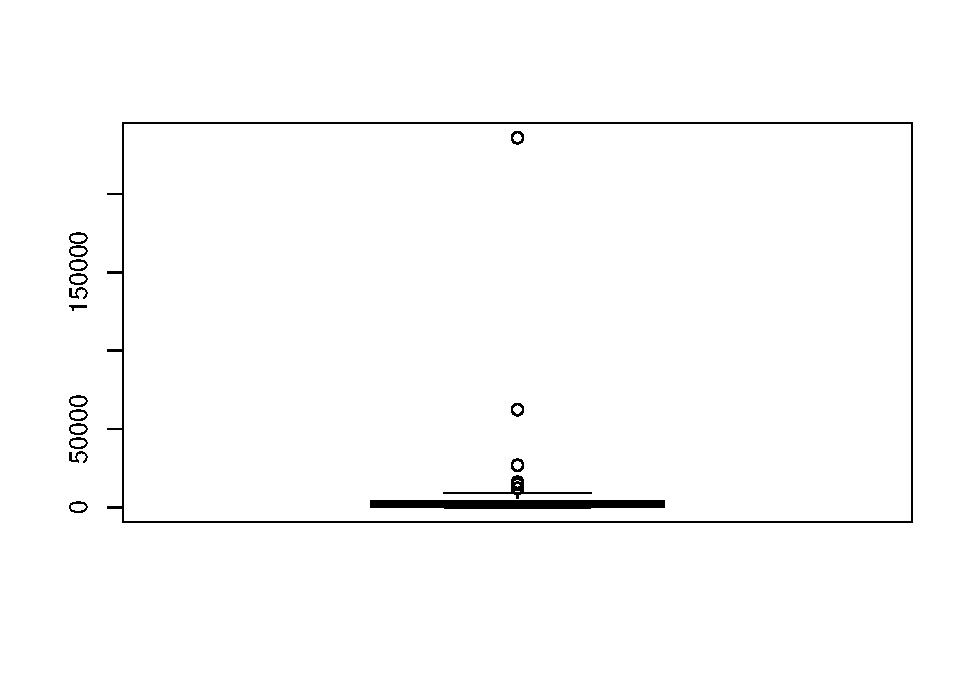
\includegraphics{_main_files/figure-latex/unnamed-chunk-77-1.pdf}

Boite à moustache du logarithme de ces valeurs

\begin{Shaded}
\begin{Highlighting}[]
\FunctionTok{boxplot}\NormalTok{(}\FunctionTok{log}\NormalTok{(exprs}\SpecialCharTok{$}\NormalTok{WT1))}
\end{Highlighting}
\end{Shaded}

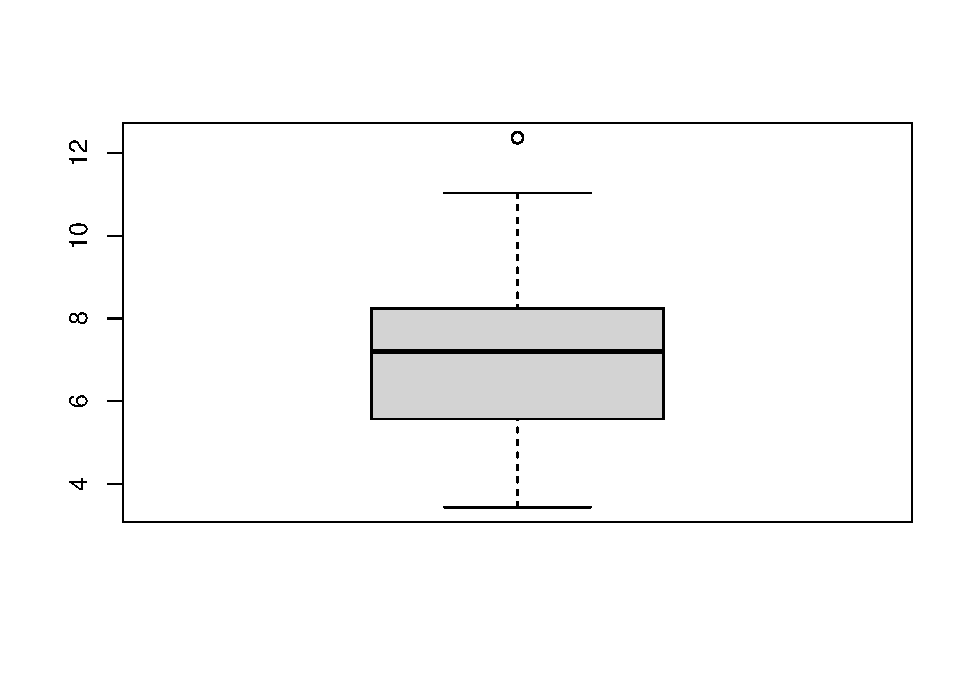
\includegraphics{_main_files/figure-latex/unnamed-chunk-78-1.pdf}

\begin{Shaded}
\begin{Highlighting}[]
\FunctionTok{boxplot}\NormalTok{(}\FunctionTok{log2}\NormalTok{(exprs}\SpecialCharTok{$}\NormalTok{WT1))}
\end{Highlighting}
\end{Shaded}

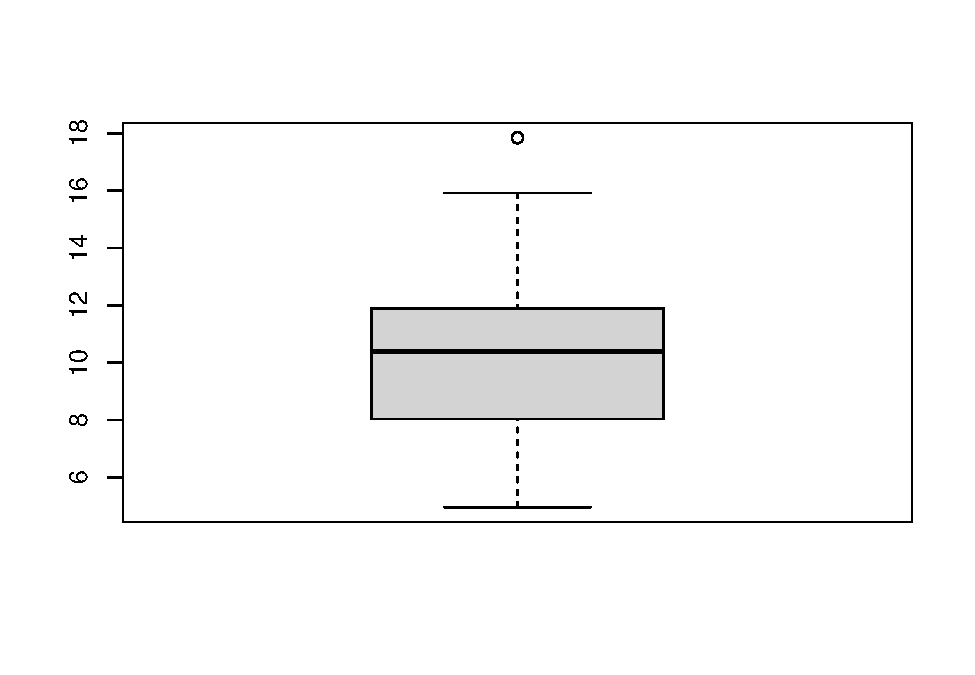
\includegraphics{_main_files/figure-latex/unnamed-chunk-79-1.pdf}

\begin{Shaded}
\begin{Highlighting}[]
\FunctionTok{boxplot}\NormalTok{(}\FunctionTok{log10}\NormalTok{(exprs}\SpecialCharTok{$}\NormalTok{WT1))}
\end{Highlighting}
\end{Shaded}

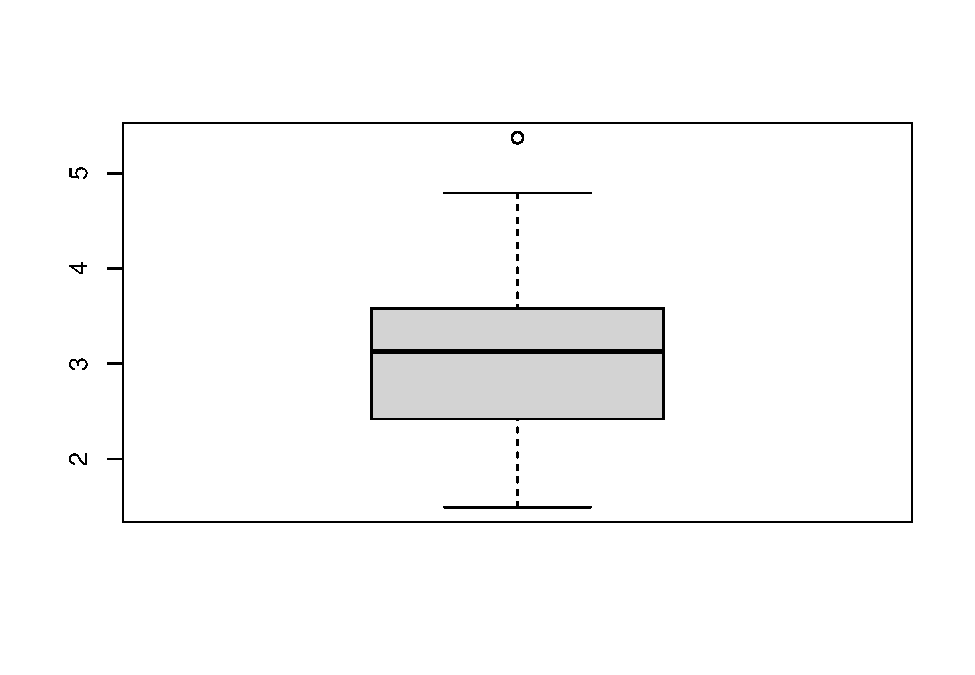
\includegraphics{_main_files/figure-latex/unnamed-chunk-80-1.pdf}

Boite à moustache des valeurs d'expression pour les 4 échantillons

\begin{Shaded}
\begin{Highlighting}[]
\FunctionTok{boxplot}\NormalTok{(exprs)}
\end{Highlighting}
\end{Shaded}

\begin{Shaded}
\begin{Highlighting}[]
\DocumentationTok{\#\# ignorer la première colonne}
\FunctionTok{boxplot}\NormalTok{(exprs[,}\SpecialCharTok{{-}}\DecValTok{1}\NormalTok{])     }
\end{Highlighting}
\end{Shaded}

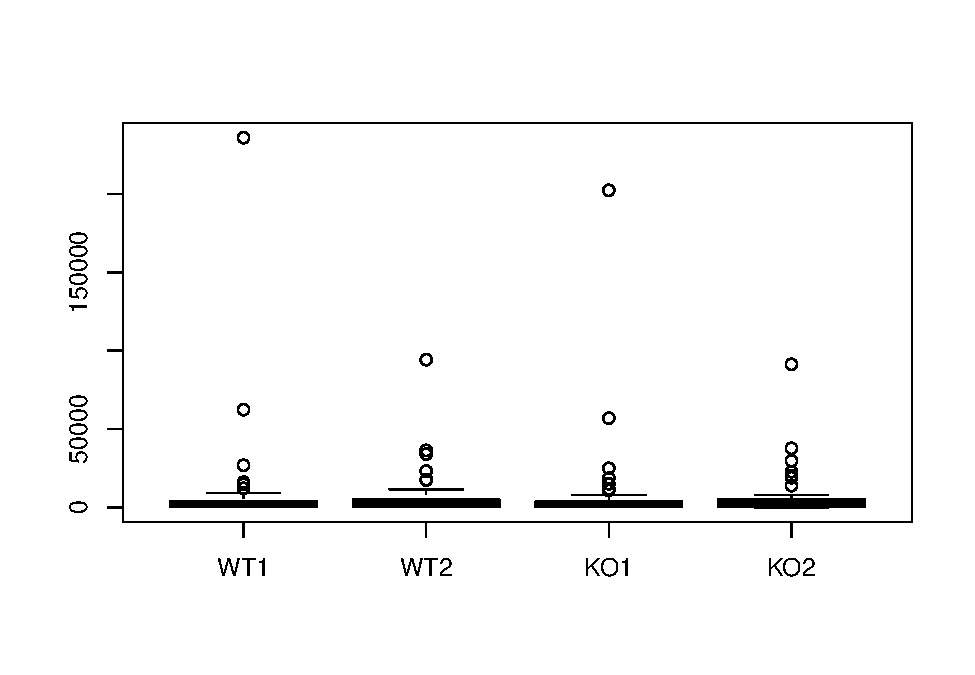
\includegraphics{_main_files/figure-latex/unnamed-chunk-81-1.pdf}

\begin{Shaded}
\begin{Highlighting}[]
\FunctionTok{boxplot}\NormalTok{(}\FunctionTok{log2}\NormalTok{(exprs[,}\SpecialCharTok{{-}}\DecValTok{1}\NormalTok{]))}
\end{Highlighting}
\end{Shaded}

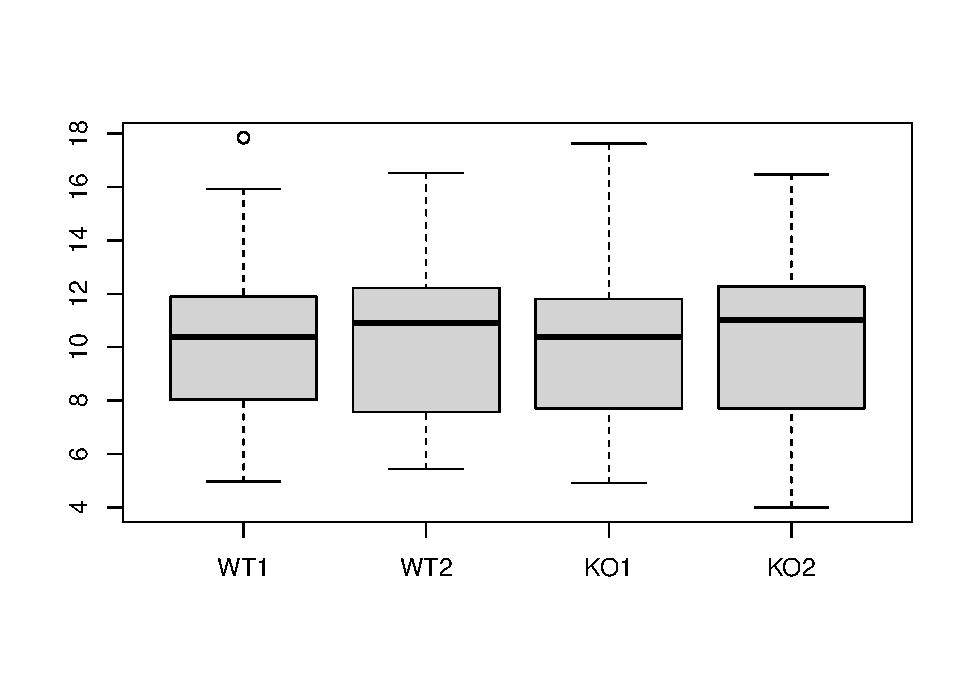
\includegraphics{_main_files/figure-latex/unnamed-chunk-82-1.pdf}

\begin{Shaded}
\begin{Highlighting}[]
\FunctionTok{boxplot}\NormalTok{(exprs[,}\SpecialCharTok{{-}}\DecValTok{1}\NormalTok{], }\AttributeTok{log =} \StringTok{"y"}\NormalTok{)}
\end{Highlighting}
\end{Shaded}

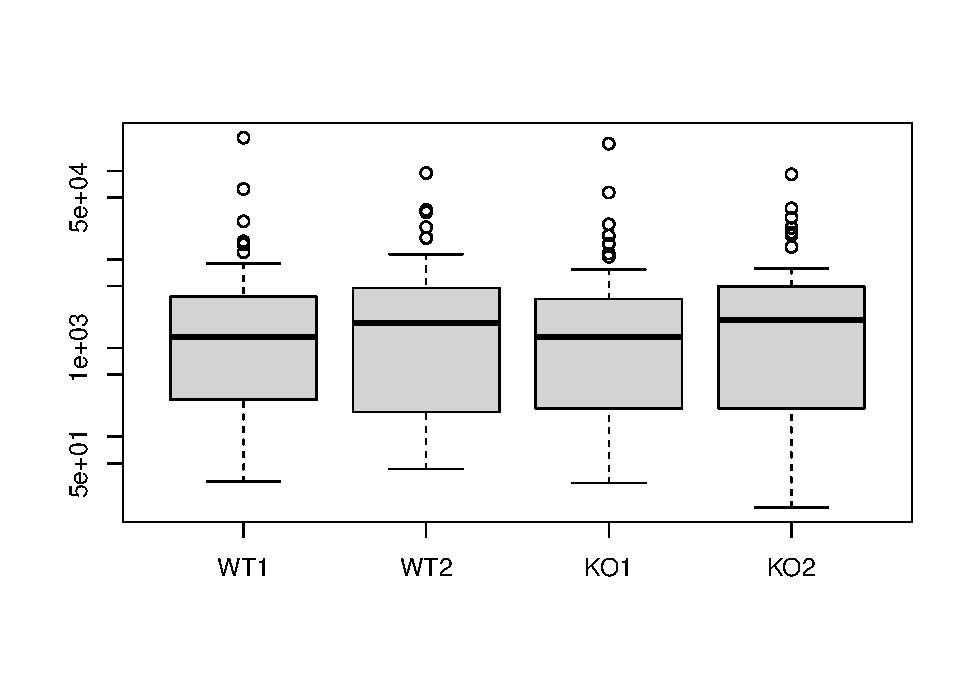
\includegraphics{_main_files/figure-latex/unnamed-chunk-83-1.pdf}

\begin{Shaded}
\begin{Highlighting}[]
\DocumentationTok{\#\# afficher les étiquettes des axes horizontalement}
\FunctionTok{boxplot}\NormalTok{(exprs[,}\SpecialCharTok{{-}}\DecValTok{1}\NormalTok{], }\AttributeTok{log =} \StringTok{"y"}\NormalTok{, }\AttributeTok{las =} \DecValTok{1}\NormalTok{) }
\end{Highlighting}
\end{Shaded}

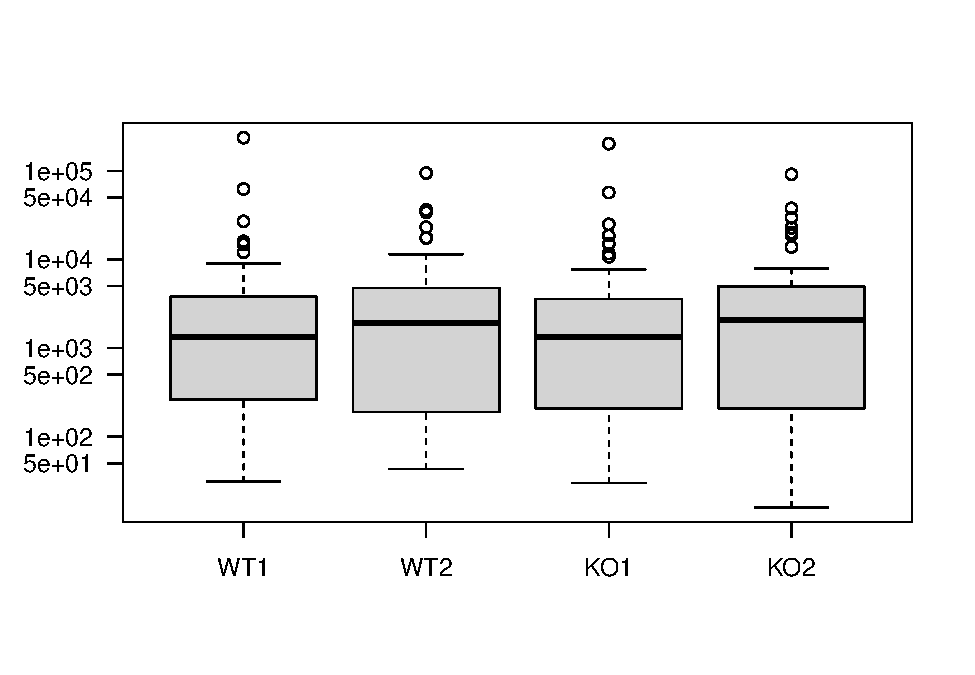
\includegraphics{_main_files/figure-latex/unnamed-chunk-84-1.pdf}

\begin{Shaded}
\begin{Highlighting}[]
\DocumentationTok{\#\# Encore plus beau}
\FunctionTok{boxplot}\NormalTok{(exprs[,}\SpecialCharTok{{-}}\DecValTok{1}\NormalTok{], }\AttributeTok{log =} \StringTok{"x"}\NormalTok{, }\AttributeTok{las =} \DecValTok{1}\NormalTok{, }\AttributeTok{horizontal =} \ConstantTok{TRUE}\NormalTok{) }
\end{Highlighting}
\end{Shaded}

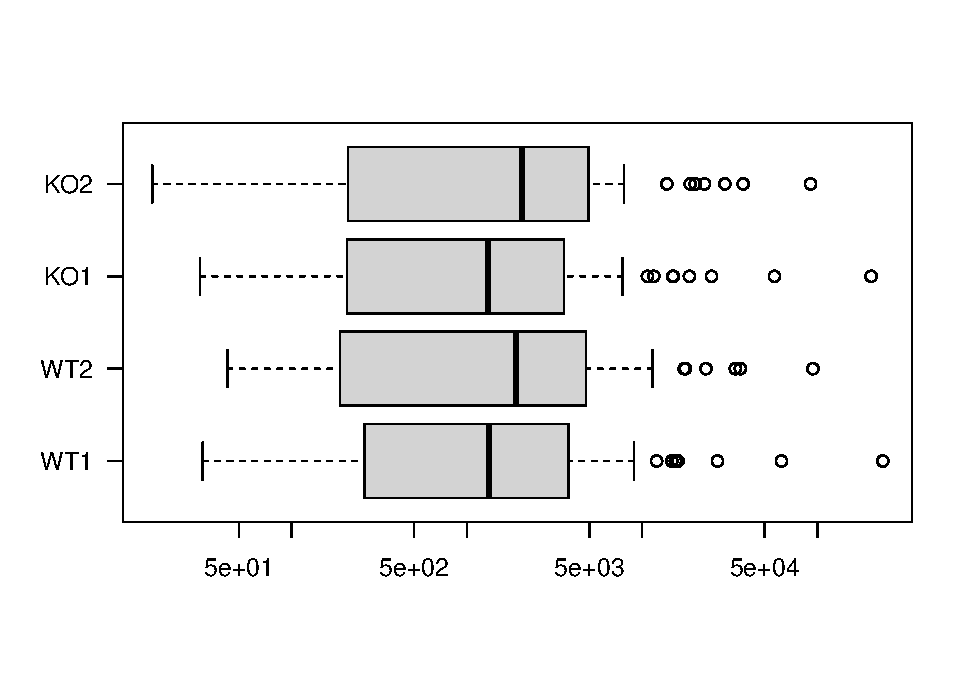
\includegraphics{_main_files/figure-latex/unnamed-chunk-85-1.pdf}

\hypertarget{nuage-de-points}{%
\section{Nuage de points}\label{nuage-de-points}}

Expressions KO1 vs WT1

\begin{Shaded}
\begin{Highlighting}[]
\FunctionTok{plot}\NormalTok{(}\AttributeTok{x =} \FunctionTok{log}\NormalTok{(exprs}\SpecialCharTok{$}\NormalTok{WT1), }\AttributeTok{y =} \FunctionTok{log}\NormalTok{(exprs}\SpecialCharTok{$}\NormalTok{KO1))}
\end{Highlighting}
\end{Shaded}

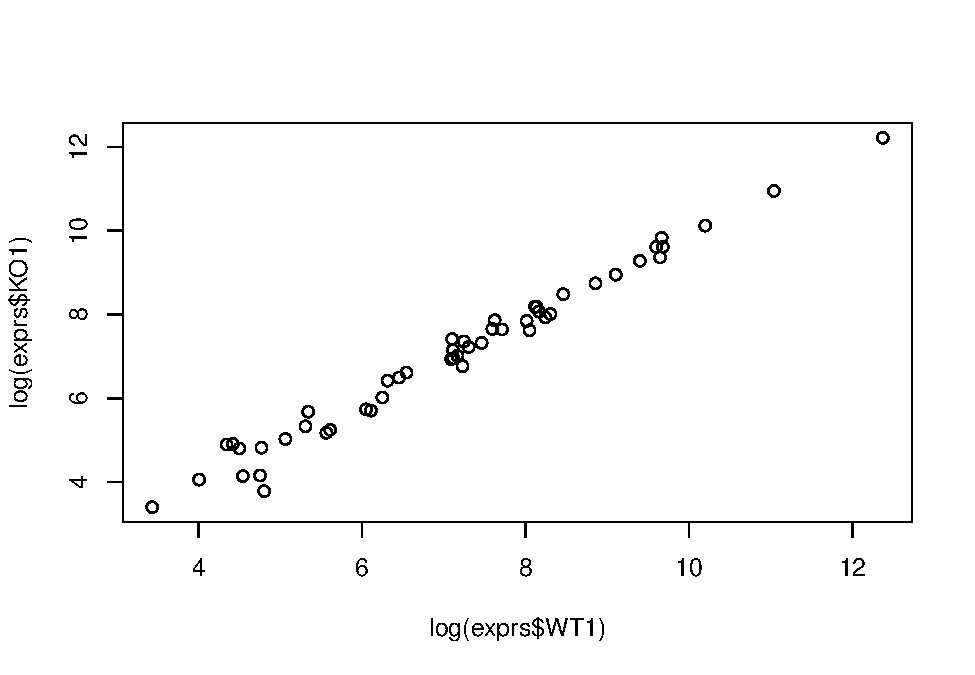
\includegraphics{_main_files/figure-latex/unnamed-chunk-86-1.pdf}

Personnalisation des paramètres graphiques

\begin{Shaded}
\begin{Highlighting}[]
\FunctionTok{plot}\NormalTok{(}\AttributeTok{x =} \FunctionTok{log}\NormalTok{(exprs}\SpecialCharTok{$}\NormalTok{WT1),                }\DocumentationTok{\#\# données pour l’abscisse}
     \AttributeTok{y =} \FunctionTok{log}\NormalTok{(exprs}\SpecialCharTok{$}\NormalTok{KO1),                    }\DocumentationTok{\#\# données pour l’ordonnée}
     \AttributeTok{main =} \StringTok{"Expression KO1 vs WT1"}\NormalTok{,    }\DocumentationTok{\#\# Titre principal}
     \AttributeTok{xlab =} \StringTok{"WT1"}\NormalTok{,                      }\DocumentationTok{\#\# légende de l’axe X}
     \AttributeTok{ylab =} \StringTok{"KO1"}\NormalTok{,                      }\DocumentationTok{\#\# légende de l’axe Y}
     \AttributeTok{pch =} \DecValTok{16}\NormalTok{,                          }\DocumentationTok{\#\# caractère pour marquer les points}
     \AttributeTok{las =} \DecValTok{1}\NormalTok{,                           }\DocumentationTok{\#\# écrire les échelles horizontalement}
     \AttributeTok{col =} \StringTok{"red"}\NormalTok{)                       }\DocumentationTok{\#\# couleur des points}
\FunctionTok{grid}\NormalTok{()                              }\DocumentationTok{\#\# ajout d’une grille}
\FunctionTok{abline}\NormalTok{(}\AttributeTok{a =} \DecValTok{0}\NormalTok{, }\AttributeTok{b =} \DecValTok{1}\NormalTok{)                        }\DocumentationTok{\#\# ajouter la droite X = Y (intercept a = 0, pente b = 1).}
\end{Highlighting}
\end{Shaded}

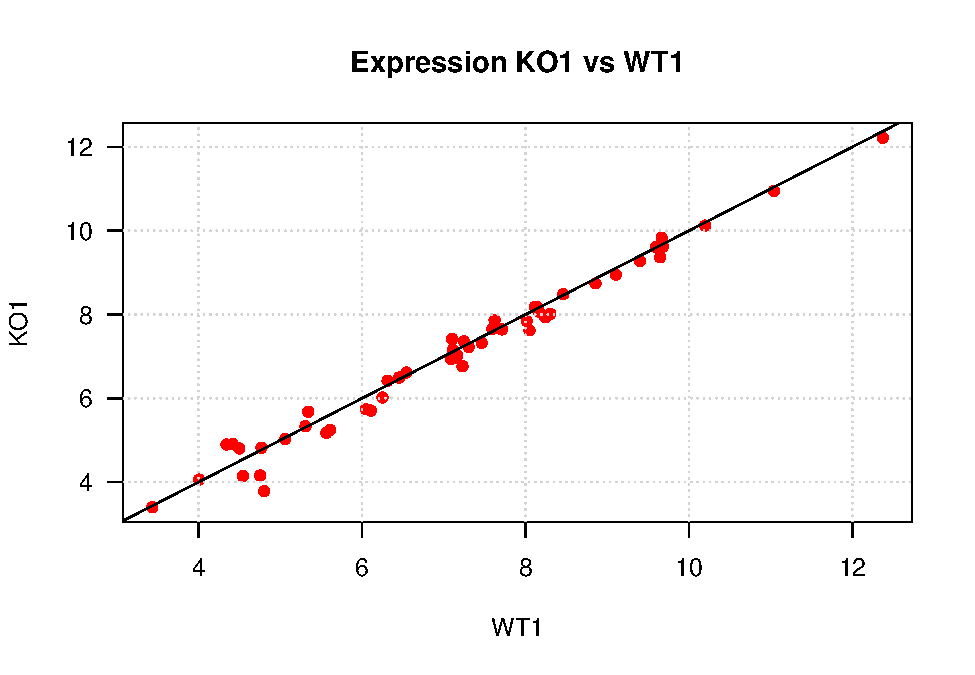
\includegraphics{_main_files/figure-latex/unnamed-chunk-87-1.pdf}

\hypertarget{analyse-dexpression-diffuxe9rentielle-ma-plot}{%
\chapter{Analyse d'expression différentielle : MA-plot}\label{analyse-dexpression-diffuxe9rentielle-ma-plot}}

\hypertarget{cest-quoi-un-ma-plot}{%
\section{C'est quoi un MA plot}\label{cest-quoi-un-ma-plot}}

\hypertarget{nos-data}{%
\subsection{Nos data}\label{nos-data}}

\begin{Shaded}
\begin{Highlighting}[]
\FunctionTok{head}\NormalTok{(exprs, }\DecValTok{10}\NormalTok{)}
\end{Highlighting}
\end{Shaded}

\begin{verbatim}
##                 id    WT1   WT2    KO1   KO2
## 1  ENSG00000034510 235960 94264 202381 91336
## 2  ENSG00000064201    116    71     64    56
## 3  ENSG00000065717    118   174    124   182
## 4  ENSG00000099958    450   655    301   472
## 5  ENSG00000104164   4736  5019   4845  4934
## 6  ENSG00000104783   9002  8623   7720  7142
## 7  ENSG00000105229   1295  2744   1113  2887
## 8  ENSG00000105723   3353  7449   3589  7202
## 9  ENSG00000116199   2044  4525   2604  4902
## 10 ENSG00000118939   7022  2526   6269  3068
\end{verbatim}

\hypertarget{la-thuxe9orie}{%
\subsection{La théorie}\label{la-thuxe9orie}}

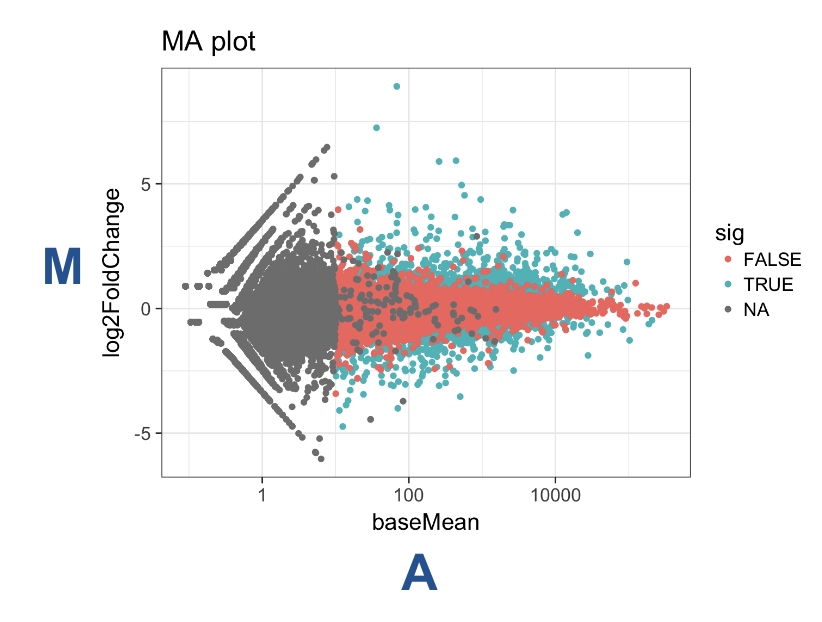
\includegraphics{images/MAplot.png}

Le MA plot représente le lien entre différence d'expression et intensité moyenne.
- M (magnitude) est le logarithme en base 2 du rapport d'expression (``log2 fold-change'')
- A (average intensity) est la moyenne des logarithmes des valeurs d'expression.

\textbf{log2 fold change, ``magnitude''}

\begin{verbatim}
M = log2(KO/WT) =  log2(KO) - log2(WT)
\end{verbatim}

\textbf{average log2 value}

\begin{verbatim}
A = ½ log2(KO x WT) = ½ (log2(KO) + log2(WT))
\end{verbatim}

\hypertarget{calculs-sur-les-colonnes}{%
\section{Calculs sur les colonnes}\label{calculs-sur-les-colonnes}}

\begin{enumerate}
\def\labelenumi{\arabic{enumi}.}
\tightlist
\item
  Calcul de moyennes par ligne (\texttt{rowMeans}) pour un sous-ensemble donné des colonnes (WT1 et WT2).
\end{enumerate}

\begin{Shaded}
\begin{Highlighting}[]
\FunctionTok{rowMeans}\NormalTok{(exprs[   , }\FunctionTok{c}\NormalTok{(}\StringTok{"WT1"}\NormalTok{,}\StringTok{"WT2"}\NormalTok{)])}
\end{Highlighting}
\end{Shaded}

\begin{verbatim}
##  [1] 165112.0     93.5    146.0    552.5   4877.5   8812.5   2019.5   5401.0
##  [9]   3284.5   4774.0  16571.0   2954.0   2229.5  10023.5   1995.5     94.0
## [17]    531.0    164.5  16827.5    807.0  48148.5   1350.0   1117.5    409.5
## [25]   1260.0  24988.5    192.5    191.5   2748.0   3388.0   1606.0   1699.5
## [33]   2559.0    199.0  25525.0   2880.5   3309.5   4770.0    126.0     66.5
## [41]    618.0    212.0    104.0     77.5   3366.0  13460.0   3133.0   1287.0
## [49]    293.0     65.5
\end{verbatim}

\begin{enumerate}
\def\labelenumi{\arabic{enumi}.}
\setcounter{enumi}{1}
\tightlist
\item
  Ajout de colonnes avec les expressions moyennes des WT et des KO
\end{enumerate}

\begin{Shaded}
\begin{Highlighting}[]
\NormalTok{exprs}\SpecialCharTok{$}\NormalTok{meanWT }\OtherTok{\textless{}{-}} \FunctionTok{rowMeans}\NormalTok{(exprs[   , }\FunctionTok{c}\NormalTok{(}\StringTok{"WT1"}\NormalTok{,}\StringTok{"WT2"}\NormalTok{)])}
\NormalTok{exprs}\SpecialCharTok{$}\NormalTok{meanKO }\OtherTok{\textless{}{-}} \FunctionTok{rowMeans}\NormalTok{(exprs[   , }\FunctionTok{c}\NormalTok{(}\StringTok{"KO1"}\NormalTok{,}\StringTok{"KO2"}\NormalTok{)])}
\end{Highlighting}
\end{Shaded}

\begin{enumerate}
\def\labelenumi{\arabic{enumi}.}
\setcounter{enumi}{2}
\tightlist
\item
  Vérification des résultats
\end{enumerate}

\begin{Shaded}
\begin{Highlighting}[]
\FunctionTok{head}\NormalTok{(exprs) }
\end{Highlighting}
\end{Shaded}

\begin{verbatim}
##                id    WT1   WT2    KO1   KO2   meanWT   meanKO
## 1 ENSG00000034510 235960 94264 202381 91336 165112.0 146858.5
## 2 ENSG00000064201    116    71     64    56     93.5     60.0
## 3 ENSG00000065717    118   174    124   182    146.0    153.0
## 4 ENSG00000099958    450   655    301   472    552.5    386.5
## 5 ENSG00000104164   4736  5019   4845  4934   4877.5   4889.5
## 6 ENSG00000104783   9002  8623   7720  7142   8812.5   7431.0
\end{verbatim}

\begin{enumerate}
\def\labelenumi{\arabic{enumi}.}
\setcounter{enumi}{3}
\tightlist
\item
  Fold-change KO vs WT
\end{enumerate}

\begin{Shaded}
\begin{Highlighting}[]
\NormalTok{exprs}\SpecialCharTok{$}\NormalTok{FC }\OtherTok{\textless{}{-}}\NormalTok{ exprs}\SpecialCharTok{$}\NormalTok{meanKO }\SpecialCharTok{/}\NormalTok{ exprs}\SpecialCharTok{$}\NormalTok{meanWT}
\end{Highlighting}
\end{Shaded}

\begin{enumerate}
\def\labelenumi{\arabic{enumi}.}
\setcounter{enumi}{4}
\tightlist
\item
  Vérification des résultats
\end{enumerate}

\begin{Shaded}
\begin{Highlighting}[]
\FunctionTok{head}\NormalTok{(exprs) }
\end{Highlighting}
\end{Shaded}

\begin{verbatim}
##                id    WT1   WT2    KO1   KO2   meanWT   meanKO        FC
## 1 ENSG00000034510 235960 94264 202381 91336 165112.0 146858.5 0.8894478
## 2 ENSG00000064201    116    71     64    56     93.5     60.0 0.6417112
## 3 ENSG00000065717    118   174    124   182    146.0    153.0 1.0479452
## 4 ENSG00000099958    450   655    301   472    552.5    386.5 0.6995475
## 5 ENSG00000104164   4736  5019   4845  4934   4877.5   4889.5 1.0024603
## 6 ENSG00000104783   9002  8623   7720  7142   8812.5   7431.0 0.8432340
\end{verbatim}

\begin{enumerate}
\def\labelenumi{\arabic{enumi}.}
\setcounter{enumi}{5}
\tightlist
\item
  Moyenne de tous les échantillons
\end{enumerate}

\begin{Shaded}
\begin{Highlighting}[]
\NormalTok{exprs}\SpecialCharTok{$}\NormalTok{mean }\OtherTok{\textless{}{-}} \FunctionTok{rowMeans}\NormalTok{(exprs[   , }\FunctionTok{c}\NormalTok{(}\StringTok{"WT1"}\NormalTok{, }\StringTok{"WT2"}\NormalTok{, }\StringTok{"KO1"}\NormalTok{, }\StringTok{"KO2"}\NormalTok{)])}
\end{Highlighting}
\end{Shaded}

\begin{enumerate}
\def\labelenumi{\arabic{enumi}.}
\setcounter{enumi}{6}
\tightlist
\item
  Vérification des résultats
\end{enumerate}

\begin{Shaded}
\begin{Highlighting}[]
\FunctionTok{head}\NormalTok{(exprs) }
\end{Highlighting}
\end{Shaded}

\begin{verbatim}
##                id    WT1   WT2    KO1   KO2   meanWT   meanKO        FC
## 1 ENSG00000034510 235960 94264 202381 91336 165112.0 146858.5 0.8894478
## 2 ENSG00000064201    116    71     64    56     93.5     60.0 0.6417112
## 3 ENSG00000065717    118   174    124   182    146.0    153.0 1.0479452
## 4 ENSG00000099958    450   655    301   472    552.5    386.5 0.6995475
## 5 ENSG00000104164   4736  5019   4845  4934   4877.5   4889.5 1.0024603
## 6 ENSG00000104783   9002  8623   7720  7142   8812.5   7431.0 0.8432340
##        mean
## 1 155985.25
## 2     76.75
## 3    149.50
## 4    469.50
## 5   4883.50
## 6   8121.75
\end{verbatim}

\hypertarget{ma-plot-log2fc-vs-intensituxe9}{%
\section{MA-plot : log2FC vs intensité}\label{ma-plot-log2fc-vs-intensituxe9}}

\hypertarget{calcul-de-m-et-a}{%
\subsection{Calcul de M et A}\label{calcul-de-m-et-a}}

\begin{Shaded}
\begin{Highlighting}[]
\NormalTok{exprs}\SpecialCharTok{$}\NormalTok{M }\OtherTok{\textless{}{-}} \FunctionTok{log2}\NormalTok{(exprs}\SpecialCharTok{$}\NormalTok{FC)}
\NormalTok{exprs}\SpecialCharTok{$}\NormalTok{A }\OtherTok{\textless{}{-}}\NormalTok{ (}\FunctionTok{log2}\NormalTok{(exprs}\SpecialCharTok{$}\NormalTok{meanKO) }\SpecialCharTok{+} \FunctionTok{log2}\NormalTok{(exprs}\SpecialCharTok{$}\NormalTok{meanWT)) }\SpecialCharTok{/}\DecValTok{2}
\end{Highlighting}
\end{Shaded}

\hypertarget{visualisation}{%
\subsection{Visualisation}\label{visualisation}}

On peut ensuite dessiner un nuage de points (en l'agrémentant un peu)

\begin{Shaded}
\begin{Highlighting}[]
\FunctionTok{plot}\NormalTok{(}\AttributeTok{x =}\NormalTok{ exprs}\SpecialCharTok{$}\NormalTok{A, }\AttributeTok{y =}\NormalTok{ exprs}\SpecialCharTok{$}\NormalTok{M, }\AttributeTok{main =} \StringTok{"MA plot"}\NormalTok{,}
       \AttributeTok{col =} \StringTok{"blue"}\NormalTok{, }\AttributeTok{pch =} \DecValTok{16}\NormalTok{, }\AttributeTok{xlab =} \StringTok{"A = intensity"}\NormalTok{, }\AttributeTok{ylab =} \StringTok{"M = log2FC"}\NormalTok{)}
\FunctionTok{grid}\NormalTok{(}\AttributeTok{lty =} \StringTok{"solid"}\NormalTok{, }\AttributeTok{col =} \StringTok{"lightgray"}\NormalTok{)}
\FunctionTok{abline}\NormalTok{(}\AttributeTok{h =} \DecValTok{0}\NormalTok{)}
\end{Highlighting}
\end{Shaded}

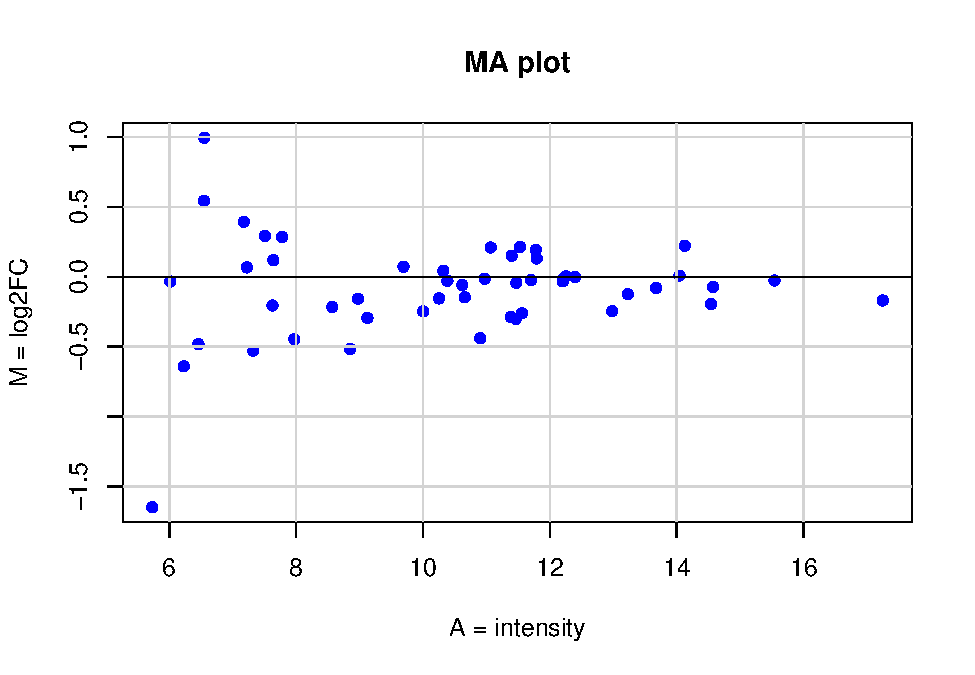
\includegraphics{_main_files/figure-latex/unnamed-chunk-97-1.pdf}

\hypertarget{appliquer-une-fonction-sur-les-lignescolonnes}{%
\section{Appliquer une fonction sur les lignes/colonnes}\label{appliquer-une-fonction-sur-les-lignescolonnes}}

\hypertarget{appliquer-une-fonction-moyenne-variance-sur-chaque-ligne-dun-tableau}{%
\subsection{Appliquer une fonction (moyenne, variance, \ldots) sur chaque ligne d'un tableau}\label{appliquer-une-fonction-moyenne-variance-sur-chaque-ligne-dun-tableau}}

\begin{Shaded}
\begin{Highlighting}[]
\NormalTok{mean\_per\_row }\OtherTok{\textless{}{-}} \FunctionTok{apply}\NormalTok{(exprs[ , }\FunctionTok{c}\NormalTok{(}\StringTok{"WT1"}\NormalTok{, }\StringTok{"WT2"}\NormalTok{, }\StringTok{"KO1"}\NormalTok{, }\StringTok{"KO2"}\NormalTok{)], }\DecValTok{1}\NormalTok{, mean)}

\NormalTok{mean\_per\_row }\OtherTok{\textless{}{-}} \FunctionTok{apply}\NormalTok{(exprs[ , }\FunctionTok{c}\NormalTok{(}\DecValTok{2}\NormalTok{, }\DecValTok{3}\NormalTok{, }\DecValTok{4}\NormalTok{, }\DecValTok{5}\NormalTok{)], }\DecValTok{1}\NormalTok{, mean)}
  
\NormalTok{mean\_per\_row }\OtherTok{\textless{}{-}} \FunctionTok{apply}\NormalTok{(exprs[ , }\SpecialCharTok{{-}}\DecValTok{1}\NormalTok{ ], }\DecValTok{1}\NormalTok{, mean)}

\NormalTok{mean\_per\_row }\OtherTok{\textless{}{-}} \FunctionTok{apply}\NormalTok{(exprs[ , }\FunctionTok{which}\NormalTok{(}\FunctionTok{sapply}\NormalTok{(exprs, class) }\SpecialCharTok{!=} \StringTok{"factor"}\NormalTok{)], }\DecValTok{1}\NormalTok{, mean)}
\end{Highlighting}
\end{Shaded}

\begin{verbatim}
## Warning in mean.default(newX[, i], ...): argument is not numeric or logical:
## returning NA

## Warning in mean.default(newX[, i], ...): argument is not numeric or logical:
## returning NA

## Warning in mean.default(newX[, i], ...): argument is not numeric or logical:
## returning NA

## Warning in mean.default(newX[, i], ...): argument is not numeric or logical:
## returning NA

## Warning in mean.default(newX[, i], ...): argument is not numeric or logical:
## returning NA

## Warning in mean.default(newX[, i], ...): argument is not numeric or logical:
## returning NA

## Warning in mean.default(newX[, i], ...): argument is not numeric or logical:
## returning NA

## Warning in mean.default(newX[, i], ...): argument is not numeric or logical:
## returning NA

## Warning in mean.default(newX[, i], ...): argument is not numeric or logical:
## returning NA

## Warning in mean.default(newX[, i], ...): argument is not numeric or logical:
## returning NA

## Warning in mean.default(newX[, i], ...): argument is not numeric or logical:
## returning NA

## Warning in mean.default(newX[, i], ...): argument is not numeric or logical:
## returning NA

## Warning in mean.default(newX[, i], ...): argument is not numeric or logical:
## returning NA

## Warning in mean.default(newX[, i], ...): argument is not numeric or logical:
## returning NA

## Warning in mean.default(newX[, i], ...): argument is not numeric or logical:
## returning NA

## Warning in mean.default(newX[, i], ...): argument is not numeric or logical:
## returning NA

## Warning in mean.default(newX[, i], ...): argument is not numeric or logical:
## returning NA

## Warning in mean.default(newX[, i], ...): argument is not numeric or logical:
## returning NA

## Warning in mean.default(newX[, i], ...): argument is not numeric or logical:
## returning NA

## Warning in mean.default(newX[, i], ...): argument is not numeric or logical:
## returning NA

## Warning in mean.default(newX[, i], ...): argument is not numeric or logical:
## returning NA

## Warning in mean.default(newX[, i], ...): argument is not numeric or logical:
## returning NA

## Warning in mean.default(newX[, i], ...): argument is not numeric or logical:
## returning NA

## Warning in mean.default(newX[, i], ...): argument is not numeric or logical:
## returning NA

## Warning in mean.default(newX[, i], ...): argument is not numeric or logical:
## returning NA

## Warning in mean.default(newX[, i], ...): argument is not numeric or logical:
## returning NA

## Warning in mean.default(newX[, i], ...): argument is not numeric or logical:
## returning NA

## Warning in mean.default(newX[, i], ...): argument is not numeric or logical:
## returning NA

## Warning in mean.default(newX[, i], ...): argument is not numeric or logical:
## returning NA

## Warning in mean.default(newX[, i], ...): argument is not numeric or logical:
## returning NA

## Warning in mean.default(newX[, i], ...): argument is not numeric or logical:
## returning NA

## Warning in mean.default(newX[, i], ...): argument is not numeric or logical:
## returning NA

## Warning in mean.default(newX[, i], ...): argument is not numeric or logical:
## returning NA

## Warning in mean.default(newX[, i], ...): argument is not numeric or logical:
## returning NA

## Warning in mean.default(newX[, i], ...): argument is not numeric or logical:
## returning NA

## Warning in mean.default(newX[, i], ...): argument is not numeric or logical:
## returning NA

## Warning in mean.default(newX[, i], ...): argument is not numeric or logical:
## returning NA

## Warning in mean.default(newX[, i], ...): argument is not numeric or logical:
## returning NA

## Warning in mean.default(newX[, i], ...): argument is not numeric or logical:
## returning NA

## Warning in mean.default(newX[, i], ...): argument is not numeric or logical:
## returning NA

## Warning in mean.default(newX[, i], ...): argument is not numeric or logical:
## returning NA

## Warning in mean.default(newX[, i], ...): argument is not numeric or logical:
## returning NA

## Warning in mean.default(newX[, i], ...): argument is not numeric or logical:
## returning NA

## Warning in mean.default(newX[, i], ...): argument is not numeric or logical:
## returning NA

## Warning in mean.default(newX[, i], ...): argument is not numeric or logical:
## returning NA

## Warning in mean.default(newX[, i], ...): argument is not numeric or logical:
## returning NA

## Warning in mean.default(newX[, i], ...): argument is not numeric or logical:
## returning NA

## Warning in mean.default(newX[, i], ...): argument is not numeric or logical:
## returning NA

## Warning in mean.default(newX[, i], ...): argument is not numeric or logical:
## returning NA

## Warning in mean.default(newX[, i], ...): argument is not numeric or logical:
## returning NA
\end{verbatim}

\begin{Shaded}
\begin{Highlighting}[]
\NormalTok{var\_per\_row }\OtherTok{\textless{}{-}} \FunctionTok{apply}\NormalTok{(exprs[ , }\FunctionTok{c}\NormalTok{(}\StringTok{"WT1"}\NormalTok{, }\StringTok{"WT2"}\NormalTok{, }\StringTok{"KO1"}\NormalTok{, }\StringTok{"KO2"}\NormalTok{)], }\DecValTok{1}\NormalTok{, var)}
\end{Highlighting}
\end{Shaded}

\hypertarget{appliquer-une-fonction-moyenne-variance-sur-chaque-colonne-dun-tableau}{%
\subsection{Appliquer une fonction (moyenne, variance, \ldots) sur chaque colonne d'un tableau}\label{appliquer-une-fonction-moyenne-variance-sur-chaque-colonne-dun-tableau}}

\begin{Shaded}
\begin{Highlighting}[]
\NormalTok{mean\_per\_col }\OtherTok{\textless{}{-}} \FunctionTok{apply}\NormalTok{(exprs[ , }\FunctionTok{c}\NormalTok{(}\StringTok{"WT1"}\NormalTok{, }\StringTok{"WT2"}\NormalTok{, }\StringTok{"KO1"}\NormalTok{, }\StringTok{"KO2"}\NormalTok{)], }\DecValTok{2}\NormalTok{, mean)}

\NormalTok{var\_per\_col }\OtherTok{\textless{}{-}} \FunctionTok{apply}\NormalTok{(exprs[ , }\FunctionTok{c}\NormalTok{(}\StringTok{"WT1"}\NormalTok{, }\StringTok{"WT2"}\NormalTok{, }\StringTok{"KO1"}\NormalTok{, }\StringTok{"KO2"}\NormalTok{)], }\DecValTok{2}\NormalTok{, var)}
\end{Highlighting}
\end{Shaded}

\hypertarget{intuxe9gration-des-donnuxe9es}{%
\chapter{Intégration des données}\label{intuxe9gration-des-donnuxe9es}}

\hypertarget{charger-les-annotations-des-guxe8nes}{%
\section{Charger les annotations des gènes}\label{charger-les-annotations-des-guxe8nes}}

\begin{Shaded}
\begin{Highlighting}[]
\FunctionTok{read.table}\NormalTok{(}\AttributeTok{file =} \StringTok{"annotation.csv"}\NormalTok{) }
\end{Highlighting}
\end{Shaded}

\begin{verbatim}
##                                                      V1
## 1                         id;name;chr;start;stop;strand
## 2            ENSG00000225630;MTND2P28;1;629640;630683;+
## 3        ENSG00000134198;TSPAN2;1;115048011;115089500;-
## 4        ENSG00000116199;FAM20B;1;179025804;179076562;+
## 5        ENSG00000119285;HEATR1;1;236549005;236604504;-
## 6          ENSG00000034510;TMSB10;2;84905625;84906675;+
## 7          ENSG00000198586;TLK1;2;170990823;171231314;-
## 8            ENSG00000157036;EXOG;3;38496127;38542161;+
## 9           ENSG00000157869;RAB28;4;13361354;13484365;-
## 10   ENSG00000250202;RP11-397E7.2;4;86876338;86876652;+
## 11        ENSG00000169570;DTWD2;5;118837322;118988545;-
## 12    ENSG00000269293;ZSCAN16-AS1;6;28121795;28137293;-
## 13        ENSG00000197081;IGF2R;6;159969099;160113507;+
## 14         ENSG00000147274;RBMX;X;136848004;136880764;-
## 15 ENSG00000253991;KB-1562D12.2;8;101528723;101529569;-
## 16          ENSG00000214121;TDPX2;9;12972843;12973438;-
## 17            ENSG00000148090;AUH;9;91213815;91361913;-
## 18        ENSG00000148248;SURF4;9;133361449;133376166;-
## 19         ENSG00000064201;TSPAN32;11;2301997;2318200;+
## 20         ENSG00000183161;FANCF;11;22622519;22626787;-
## 21         ENSG00000121680;PEX16;11;45909669;45918812;-
## 22         ENSG00000254470;AP5B1;11;65775893;65780802;-
## 23       ENSG00000135452;TSPAN31;12;57738013;57750211;+
## 24      ENSG00000251106;FAM206BP;13;46270077;46270617;+
## 25         ENSG00000118939;UCHL3;13;75549480;75606020;+
## 26        ENSG00000238241;CCR12P;13;99407781;99409062;-
## 27          ENSG00000129562;DAD1;14;22564905;22589269;-
## 28        ENSG00000125384;PTGER2;14;52314305;52328606;+
## 29        ENSG00000159433;STARD9;15;42575659;42720981;+
## 30       ENSG00000104164;BLOC1S6;15;45587123;45615999;+
## 31          ENSG00000140416;TPM1;15;63042632;63071915;+
## 32        ENSG00000167005;NUDT21;16;56429133;56452199;-
## 33         ENSG00000185324;CDK10;16;89680737;89696364;+
## 34         ENSG00000161692;DBF4B;17;44708608;44752264;+
## 35        ENSG00000168517;HEXIM2;17;45160700;45170040;+
## 36        ENSG00000262814;MRPL12;17;81703357;81707526;+
## 37        ENSG00000188985;DHFRP1;18;26170726;26171284;-
## 38       ENSG00000267228;IER3IP1;18;47134656;47176281;-
## 39  ENSG00000267699;RP11-729L2.2;18;50968019;51058144;+
## 40       ENSG00000226742;HSBP1L1;18;79964561;79970822;+
## 41         ENSG00000172216;CEBPB;20;50190734;50192689;+
## 42             ENSG00000175221;MED16;19;867630;893218;-
## 43            ENSG00000065717;TLE2;19;2997638;3047635;-
## 44            ENSG00000129932;DOHH;19;3490821;3500940;-
## 45           ENSG00000105229;PIAS4;19;4007646;4039386;+
## 46 ENSG00000279329;CTD-2553L13.9;19;34675717;34677581;-
## 47         ENSG00000105723;GSK3A;19;42230186;42242625;-
## 48         ENSG00000104783;KCNN4;19;43766533;43781257;-
## 49         ENSG00000196867;ZFP28;19;56538948;56556810;+
## 50         ENSG00000099958;DERL3;22;23834503;23839128;-
## 51 ENSG00000248751;RP1-130H16.18;22;30285238;30299482;-
\end{verbatim}

Pas cool\ldots{}

\begin{Shaded}
\begin{Highlighting}[]
\FunctionTok{read.table}\NormalTok{(}\AttributeTok{file =} \StringTok{"annotation.csv"}\NormalTok{, }\AttributeTok{sep =} \StringTok{";"}\NormalTok{)  }
\end{Highlighting}
\end{Shaded}

\begin{verbatim}
##                 V1            V2  V3        V4        V5     V6
## 1               id          name chr     start      stop strand
## 2  ENSG00000225630      MTND2P28   1    629640    630683      +
## 3  ENSG00000134198        TSPAN2   1 115048011 115089500      -
## 4  ENSG00000116199        FAM20B   1 179025804 179076562      +
## 5  ENSG00000119285        HEATR1   1 236549005 236604504      -
## 6  ENSG00000034510        TMSB10   2  84905625  84906675      +
## 7  ENSG00000198586          TLK1   2 170990823 171231314      -
## 8  ENSG00000157036          EXOG   3  38496127  38542161      +
## 9  ENSG00000157869         RAB28   4  13361354  13484365      -
## 10 ENSG00000250202  RP11-397E7.2   4  86876338  86876652      +
## 11 ENSG00000169570         DTWD2   5 118837322 118988545      -
## 12 ENSG00000269293   ZSCAN16-AS1   6  28121795  28137293      -
## 13 ENSG00000197081         IGF2R   6 159969099 160113507      +
## 14 ENSG00000147274          RBMX   X 136848004 136880764      -
## 15 ENSG00000253991  KB-1562D12.2   8 101528723 101529569      -
## 16 ENSG00000214121         TDPX2   9  12972843  12973438      -
## 17 ENSG00000148090           AUH   9  91213815  91361913      -
## 18 ENSG00000148248         SURF4   9 133361449 133376166      -
## 19 ENSG00000064201       TSPAN32  11   2301997   2318200      +
## 20 ENSG00000183161         FANCF  11  22622519  22626787      -
## 21 ENSG00000121680         PEX16  11  45909669  45918812      -
## 22 ENSG00000254470         AP5B1  11  65775893  65780802      -
## 23 ENSG00000135452       TSPAN31  12  57738013  57750211      +
## 24 ENSG00000251106      FAM206BP  13  46270077  46270617      +
## 25 ENSG00000118939         UCHL3  13  75549480  75606020      +
## 26 ENSG00000238241        CCR12P  13  99407781  99409062      -
## 27 ENSG00000129562          DAD1  14  22564905  22589269      -
## 28 ENSG00000125384        PTGER2  14  52314305  52328606      +
## 29 ENSG00000159433        STARD9  15  42575659  42720981      +
## 30 ENSG00000104164       BLOC1S6  15  45587123  45615999      +
## 31 ENSG00000140416          TPM1  15  63042632  63071915      +
## 32 ENSG00000167005        NUDT21  16  56429133  56452199      -
## 33 ENSG00000185324         CDK10  16  89680737  89696364      +
## 34 ENSG00000161692         DBF4B  17  44708608  44752264      +
## 35 ENSG00000168517        HEXIM2  17  45160700  45170040      +
## 36 ENSG00000262814        MRPL12  17  81703357  81707526      +
## 37 ENSG00000188985        DHFRP1  18  26170726  26171284      -
## 38 ENSG00000267228       IER3IP1  18  47134656  47176281      -
## 39 ENSG00000267699  RP11-729L2.2  18  50968019  51058144      +
## 40 ENSG00000226742       HSBP1L1  18  79964561  79970822      +
## 41 ENSG00000172216         CEBPB  20  50190734  50192689      +
## 42 ENSG00000175221         MED16  19    867630    893218      -
## 43 ENSG00000065717          TLE2  19   2997638   3047635      -
## 44 ENSG00000129932          DOHH  19   3490821   3500940      -
## 45 ENSG00000105229         PIAS4  19   4007646   4039386      +
## 46 ENSG00000279329 CTD-2553L13.9  19  34675717  34677581      -
## 47 ENSG00000105723         GSK3A  19  42230186  42242625      -
## 48 ENSG00000104783         KCNN4  19  43766533  43781257      -
## 49 ENSG00000196867         ZFP28  19  56538948  56556810      +
## 50 ENSG00000099958         DERL3  22  23834503  23839128      -
## 51 ENSG00000248751 RP1-130H16.18  22  30285238  30299482      -
\end{verbatim}

Pas encore parfait.

\begin{Shaded}
\begin{Highlighting}[]
\FunctionTok{read.table}\NormalTok{(}\AttributeTok{file =} \StringTok{"annotation.csv"}\NormalTok{, }\AttributeTok{sep =} \StringTok{";"}\NormalTok{, }\AttributeTok{header =} \ConstantTok{TRUE}\NormalTok{)}
\end{Highlighting}
\end{Shaded}

\begin{verbatim}
##                 id          name chr     start      stop strand
## 1  ENSG00000225630      MTND2P28   1    629640    630683      +
## 2  ENSG00000134198        TSPAN2   1 115048011 115089500      -
## 3  ENSG00000116199        FAM20B   1 179025804 179076562      +
## 4  ENSG00000119285        HEATR1   1 236549005 236604504      -
## 5  ENSG00000034510        TMSB10   2  84905625  84906675      +
## 6  ENSG00000198586          TLK1   2 170990823 171231314      -
## 7  ENSG00000157036          EXOG   3  38496127  38542161      +
## 8  ENSG00000157869         RAB28   4  13361354  13484365      -
## 9  ENSG00000250202  RP11-397E7.2   4  86876338  86876652      +
## 10 ENSG00000169570         DTWD2   5 118837322 118988545      -
## 11 ENSG00000269293   ZSCAN16-AS1   6  28121795  28137293      -
## 12 ENSG00000197081         IGF2R   6 159969099 160113507      +
## 13 ENSG00000147274          RBMX   X 136848004 136880764      -
## 14 ENSG00000253991  KB-1562D12.2   8 101528723 101529569      -
## 15 ENSG00000214121         TDPX2   9  12972843  12973438      -
## 16 ENSG00000148090           AUH   9  91213815  91361913      -
## 17 ENSG00000148248         SURF4   9 133361449 133376166      -
## 18 ENSG00000064201       TSPAN32  11   2301997   2318200      +
## 19 ENSG00000183161         FANCF  11  22622519  22626787      -
## 20 ENSG00000121680         PEX16  11  45909669  45918812      -
## 21 ENSG00000254470         AP5B1  11  65775893  65780802      -
## 22 ENSG00000135452       TSPAN31  12  57738013  57750211      +
## 23 ENSG00000251106      FAM206BP  13  46270077  46270617      +
## 24 ENSG00000118939         UCHL3  13  75549480  75606020      +
## 25 ENSG00000238241        CCR12P  13  99407781  99409062      -
## 26 ENSG00000129562          DAD1  14  22564905  22589269      -
## 27 ENSG00000125384        PTGER2  14  52314305  52328606      +
## 28 ENSG00000159433        STARD9  15  42575659  42720981      +
## 29 ENSG00000104164       BLOC1S6  15  45587123  45615999      +
## 30 ENSG00000140416          TPM1  15  63042632  63071915      +
## 31 ENSG00000167005        NUDT21  16  56429133  56452199      -
## 32 ENSG00000185324         CDK10  16  89680737  89696364      +
## 33 ENSG00000161692         DBF4B  17  44708608  44752264      +
## 34 ENSG00000168517        HEXIM2  17  45160700  45170040      +
## 35 ENSG00000262814        MRPL12  17  81703357  81707526      +
## 36 ENSG00000188985        DHFRP1  18  26170726  26171284      -
## 37 ENSG00000267228       IER3IP1  18  47134656  47176281      -
## 38 ENSG00000267699  RP11-729L2.2  18  50968019  51058144      +
## 39 ENSG00000226742       HSBP1L1  18  79964561  79970822      +
## 40 ENSG00000172216         CEBPB  20  50190734  50192689      +
## 41 ENSG00000175221         MED16  19    867630    893218      -
## 42 ENSG00000065717          TLE2  19   2997638   3047635      -
## 43 ENSG00000129932          DOHH  19   3490821   3500940      -
## 44 ENSG00000105229         PIAS4  19   4007646   4039386      +
## 45 ENSG00000279329 CTD-2553L13.9  19  34675717  34677581      -
## 46 ENSG00000105723         GSK3A  19  42230186  42242625      -
## 47 ENSG00000104783         KCNN4  19  43766533  43781257      -
## 48 ENSG00000196867         ZFP28  19  56538948  56556810      +
## 49 ENSG00000099958         DERL3  22  23834503  23839128      -
## 50 ENSG00000248751 RP1-130H16.18  22  30285238  30299482      -
\end{verbatim}

Parfait !

\begin{Shaded}
\begin{Highlighting}[]
\NormalTok{annot }\OtherTok{\textless{}{-}} \FunctionTok{read.table}\NormalTok{(}\AttributeTok{file =} \StringTok{"annotation.csv"}\NormalTok{, }\AttributeTok{sep =} \StringTok{";"}\NormalTok{, }\AttributeTok{header =} \ConstantTok{TRUE}\NormalTok{)}
\end{Highlighting}
\end{Shaded}

Vérifier les dimensions

\begin{Shaded}
\begin{Highlighting}[]
\FunctionTok{dim}\NormalTok{(annot)  }
\end{Highlighting}
\end{Shaded}

\begin{verbatim}
## [1] 50  6
\end{verbatim}

Afficher quelques lignes

\begin{Shaded}
\begin{Highlighting}[]
\FunctionTok{head}\NormalTok{(annot)}
\end{Highlighting}
\end{Shaded}

\begin{verbatim}
##                id     name chr     start      stop strand
## 1 ENSG00000225630 MTND2P28   1    629640    630683      +
## 2 ENSG00000134198   TSPAN2   1 115048011 115089500      -
## 3 ENSG00000116199   FAM20B   1 179025804 179076562      +
## 4 ENSG00000119285   HEATR1   1 236549005 236604504      -
## 5 ENSG00000034510   TMSB10   2  84905625  84906675      +
## 6 ENSG00000198586     TLK1   2 170990823 171231314      -
\end{verbatim}

\hypertarget{combien}{%
\section{Combien ?}\label{combien}}

\begin{itemize}
\tightlist
\item
  Combien de gènes sur le chromosome 18 ?
\item
  Combien de gènes sur le chromosome X ?
\end{itemize}

\hypertarget{solution-pour-y-ruxe9pondre}{%
\subsection{Solution pour y répondre}\label{solution-pour-y-ruxe9pondre}}

\begin{Shaded}
\begin{Highlighting}[]
\FunctionTok{table}\NormalTok{(annot}\SpecialCharTok{$}\NormalTok{chr)}
\end{Highlighting}
\end{Shaded}

\begin{verbatim}
## 
##  1 11 12 13 14 15 16 17 18 19  2 20 22  3  4  5  6  8  9  X 
##  4  4  1  3  2  3  2  3  4  8  2  1  2  1  2  1  2  1  3  1
\end{verbatim}

\begin{Shaded}
\begin{Highlighting}[]
\FunctionTok{barplot}\NormalTok{(}\FunctionTok{sort}\NormalTok{(}\FunctionTok{table}\NormalTok{(annot}\SpecialCharTok{$}\NormalTok{chr)), }\AttributeTok{horiz =} \ConstantTok{TRUE}\NormalTok{, }\AttributeTok{las =} \DecValTok{1}\NormalTok{,}
            \AttributeTok{col =} \StringTok{"lightblue"}\NormalTok{,  }\AttributeTok{xlab =} \StringTok{"Number of genes"}\NormalTok{)}
\end{Highlighting}
\end{Shaded}

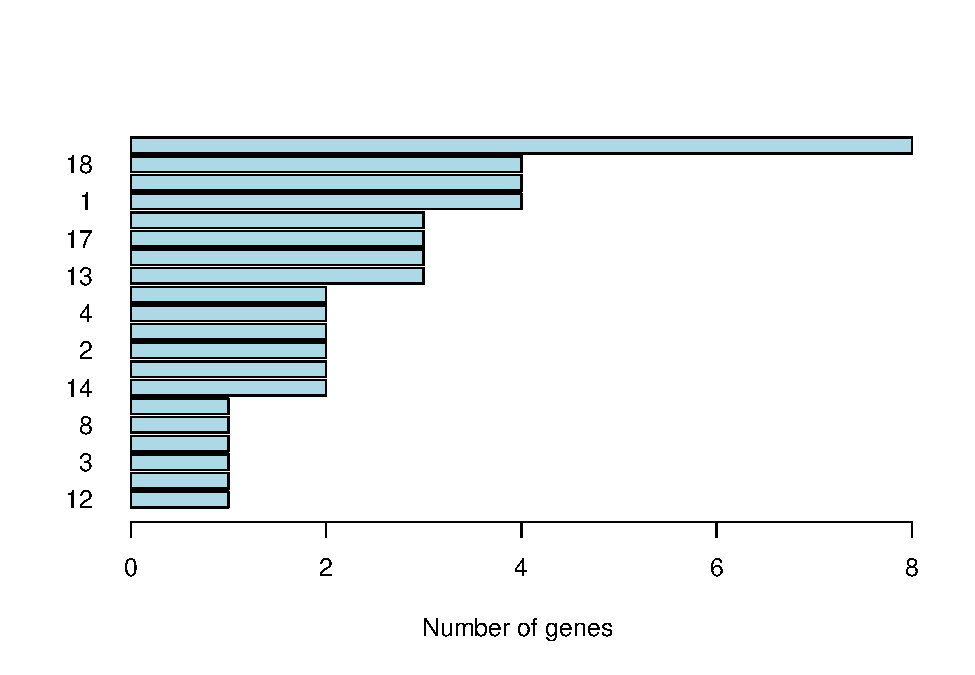
\includegraphics{_main_files/figure-latex/unnamed-chunk-107-1.pdf}

\hypertarget{ma-premiuxe8re-bioinformatique-intuxe9grative}{%
\section{Ma première bioinformatique intégrative}\label{ma-premiuxe8re-bioinformatique-intuxe9grative}}

\hypertarget{uxe9tape-1---fusionner-les-tableaux-dexpressions-et-dannotations}{%
\subsection{Étape 1 - Fusionner les tableaux d'expressions et d'annotations :}\label{uxe9tape-1---fusionner-les-tableaux-dexpressions-et-dannotations}}

\begin{Shaded}
\begin{Highlighting}[]
\NormalTok{?merge}
\end{Highlighting}
\end{Shaded}

\begin{Shaded}
\begin{Highlighting}[]
\NormalTok{exprs\_annot }\OtherTok{\textless{}{-}} \FunctionTok{merge}\NormalTok{(exprs, annot, }\AttributeTok{by =} \StringTok{"id"}\NormalTok{)}
\FunctionTok{head}\NormalTok{(exprs\_annot)}
\end{Highlighting}
\end{Shaded}

\begin{verbatim}
##                id    WT1   WT2    KO1   KO2   meanWT   meanKO        FC
## 1 ENSG00000034510 235960 94264 202381 91336 165112.0 146858.5 0.8894478
## 2 ENSG00000064201    116    71     64    56     93.5     60.0 0.6417112
## 3 ENSG00000065717    118   174    124   182    146.0    153.0 1.0479452
## 4 ENSG00000099958    450   655    301   472    552.5    386.5 0.6995475
## 5 ENSG00000104164   4736  5019   4845  4934   4877.5   4889.5 1.0024603
## 6 ENSG00000104783   9002  8623   7720  7142   8812.5   7431.0 0.8432340
##        mean           M         A    name chr    start     stop strand
## 1 155985.25 -0.16901821 17.248576  TMSB10   2 84905625 84906675      +
## 2     76.75 -0.64000386  6.226893 TSPAN32  11  2301997  2318200      +
## 3    149.50  0.06756328  7.223606    TLE2  19  2997638  3047635      -
## 4    469.50 -0.51550605  8.852078   DERL3  22 23834503 23839128      -
## 5   4883.50  0.00354507 12.253699 BLOC1S6  15 45587123 45615999      +
## 6   8121.75 -0.24599498 12.982338   KCNN4  19 43766533 43781257      -
\end{verbatim}

\hypertarget{uxe9tape-2---sous-ensemble-des-lignes-pour-lesquelles-chr-vaut-8}{%
\subsection{Étape 2 - Sous-ensemble des lignes pour lesquelles chr vaut 8 :}\label{uxe9tape-2---sous-ensemble-des-lignes-pour-lesquelles-chr-vaut-8}}

\begin{Shaded}
\begin{Highlighting}[]
\NormalTok{exprs\_chr8 }\OtherTok{\textless{}{-}}\NormalTok{ exprs\_annot[}\FunctionTok{which}\NormalTok{(exprs\_annot}\SpecialCharTok{$}\NormalTok{chr }\SpecialCharTok{==} \DecValTok{8}\NormalTok{),   ]}
\FunctionTok{print}\NormalTok{(exprs\_chr8)}
\end{Highlighting}
\end{Shaded}

\begin{verbatim}
##                 id WT1 WT2 KO1 KO2 meanWT meanKO       FC  mean         M
## 44 ENSG00000253991  77  78 134  92   77.5    113 1.458065 95.25 0.5440546
##           A         name chr     start      stop strand
## 44 6.548152 KB-1562D12.2   8 101528723 101529569      -
\end{verbatim}

\hypertarget{exporter-exprs_chr8-dans-un-fichier}{%
\subsection{Exporter exprs\_chr8 dans un fichier}\label{exporter-exprs_chr8-dans-un-fichier}}

\begin{Shaded}
\begin{Highlighting}[]
\FunctionTok{write.table}\NormalTok{(}\AttributeTok{x =}\NormalTok{ exprs\_chr8, }\AttributeTok{file =} \StringTok{"exprs\_chr8.txt"}\NormalTok{, }
   \AttributeTok{sep =} \StringTok{"}\SpecialCharTok{\textbackslash{}t}\StringTok{"}\NormalTok{, }
   \AttributeTok{row.names =} \ConstantTok{FALSE}\NormalTok{, }
   \AttributeTok{col.names =} \ConstantTok{TRUE}\NormalTok{)}
\end{Highlighting}
\end{Shaded}

\hypertarget{visualisation-1}{%
\section{Visualisation}\label{visualisation-1}}

\begin{Shaded}
\begin{Highlighting}[]
\FunctionTok{library}\NormalTok{(plotly)}
\end{Highlighting}
\end{Shaded}

\begin{verbatim}
## 
## Attaching package: 'plotly'
\end{verbatim}

\begin{verbatim}
## The following object is masked from 'package:ggplot2':
## 
##     last_plot
\end{verbatim}

\begin{verbatim}
## The following object is masked from 'package:stats':
## 
##     filter
\end{verbatim}

\begin{verbatim}
## The following object is masked from 'package:graphics':
## 
##     layout
\end{verbatim}

\begin{Shaded}
\begin{Highlighting}[]
\FunctionTok{plot\_ly}\NormalTok{(}\AttributeTok{data =}\NormalTok{ exprs\_annot, }\AttributeTok{x =} \SpecialCharTok{\textasciitilde{}}\NormalTok{A, }\AttributeTok{y =} \SpecialCharTok{\textasciitilde{}}\NormalTok{M, }\AttributeTok{text =} \FunctionTok{paste}\NormalTok{(}\StringTok{"Gene name :"}\NormalTok{, exprs\_annot}\SpecialCharTok{$}\NormalTok{name), }\AttributeTok{type =} \StringTok{\textquotesingle{}scatter\textquotesingle{}}\NormalTok{, }\AttributeTok{mode =} \StringTok{\textquotesingle{}markers\textquotesingle{}}\NormalTok{)}
\end{Highlighting}
\end{Shaded}

\hypertarget{bonus}{%
\chapter{Bonus}\label{bonus}}

Dans cette partie, nous allons produire un même graphe avec différentes approches.

\hypertarget{r-de-base}{%
\section{R de base}\label{r-de-base}}

\begin{Shaded}
\begin{Highlighting}[]
\FunctionTok{plot}\NormalTok{(}\AttributeTok{x =}\NormalTok{ exprs}\SpecialCharTok{$}\NormalTok{A, }\AttributeTok{y =}\NormalTok{ exprs}\SpecialCharTok{$}\NormalTok{M, }\AttributeTok{main =} \StringTok{"MA plot"}\NormalTok{,}
       \AttributeTok{col =} \StringTok{"blue"}\NormalTok{, }\AttributeTok{pch =} \DecValTok{16}\NormalTok{, }\AttributeTok{xlab =} \StringTok{"A = intensity"}\NormalTok{, }\AttributeTok{ylab =} \StringTok{"M = log2FC"}\NormalTok{)}
\FunctionTok{grid}\NormalTok{(}\AttributeTok{lty =} \StringTok{"solid"}\NormalTok{, }\AttributeTok{col =} \StringTok{"lightgray"}\NormalTok{)}
\FunctionTok{abline}\NormalTok{(}\AttributeTok{h =} \DecValTok{0}\NormalTok{)}
\end{Highlighting}
\end{Shaded}

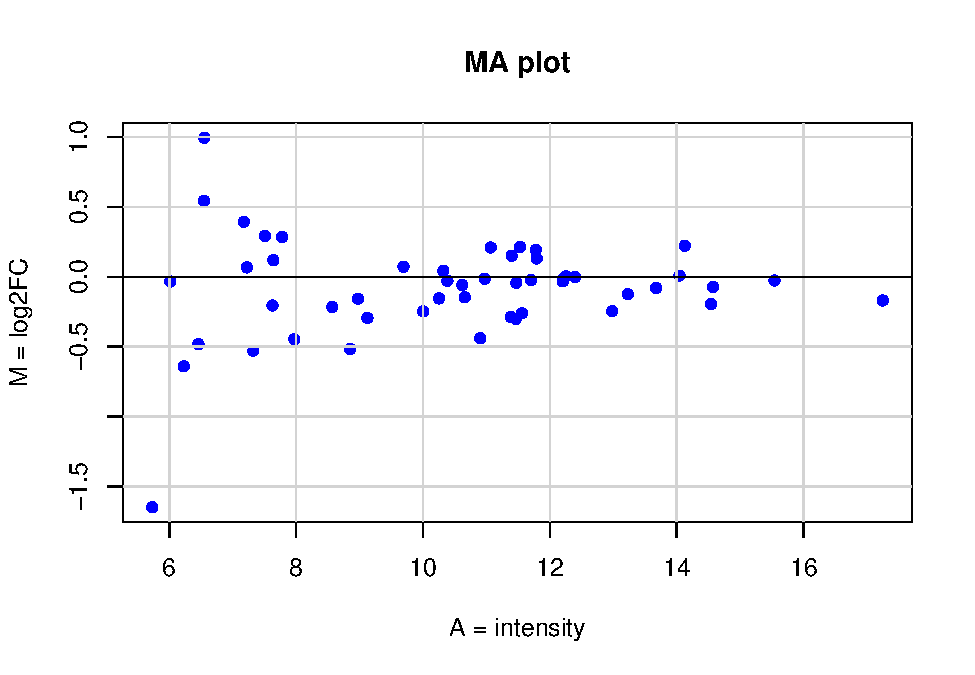
\includegraphics{_main_files/figure-latex/unnamed-chunk-113-1.pdf}
\#\# ggplot2

\begin{Shaded}
\begin{Highlighting}[]
\FunctionTok{library}\NormalTok{(ggplot2)}

\NormalTok{g }\OtherTok{\textless{}{-}} \FunctionTok{ggplot}\NormalTok{(}\AttributeTok{data =}\NormalTok{ exprs, }\FunctionTok{aes}\NormalTok{(}\AttributeTok{x =}\NormalTok{ A, }\AttributeTok{y =}\NormalTok{ M)) }\SpecialCharTok{+}
  \FunctionTok{geom\_point}\NormalTok{(}\FunctionTok{aes}\NormalTok{(A, M, }\AttributeTok{colour =} \FunctionTok{factor}\NormalTok{(}\FunctionTok{ifelse}\NormalTok{(}\FunctionTok{abs}\NormalTok{(M) }\SpecialCharTok{\textless{}=} \DecValTok{1}\NormalTok{, }\DecValTok{1}\NormalTok{,}\DecValTok{2}\NormalTok{))), }\AttributeTok{size =} \FloatTok{0.8}\NormalTok{) }\SpecialCharTok{+} 
  \FunctionTok{geom\_hline}\NormalTok{(}\AttributeTok{yintercept =} \FunctionTok{c}\NormalTok{(}\SpecialCharTok{{-}}\DecValTok{1}\NormalTok{,}\DecValTok{1}\NormalTok{)) }\SpecialCharTok{+}
  \FunctionTok{scale\_color\_manual}\NormalTok{(}\AttributeTok{values =} \FunctionTok{c}\NormalTok{(}\StringTok{"black"}\NormalTok{,}\StringTok{"red"}\NormalTok{)) }\SpecialCharTok{+}
  \FunctionTok{ggtitle}\NormalTok{(}\StringTok{"MA plot"}\NormalTok{) }\SpecialCharTok{+} 
  \FunctionTok{labs}\NormalTok{(}\AttributeTok{y =} \StringTok{"M = log2FC"}\NormalTok{, }\AttributeTok{x =} \StringTok{"A = intensity"}\NormalTok{) }\SpecialCharTok{+} 
  \FunctionTok{theme\_light}\NormalTok{() }\SpecialCharTok{+} \FunctionTok{theme}\NormalTok{(}\AttributeTok{legend.position =} \StringTok{"none"}\NormalTok{)}
\NormalTok{g}
\end{Highlighting}
\end{Shaded}

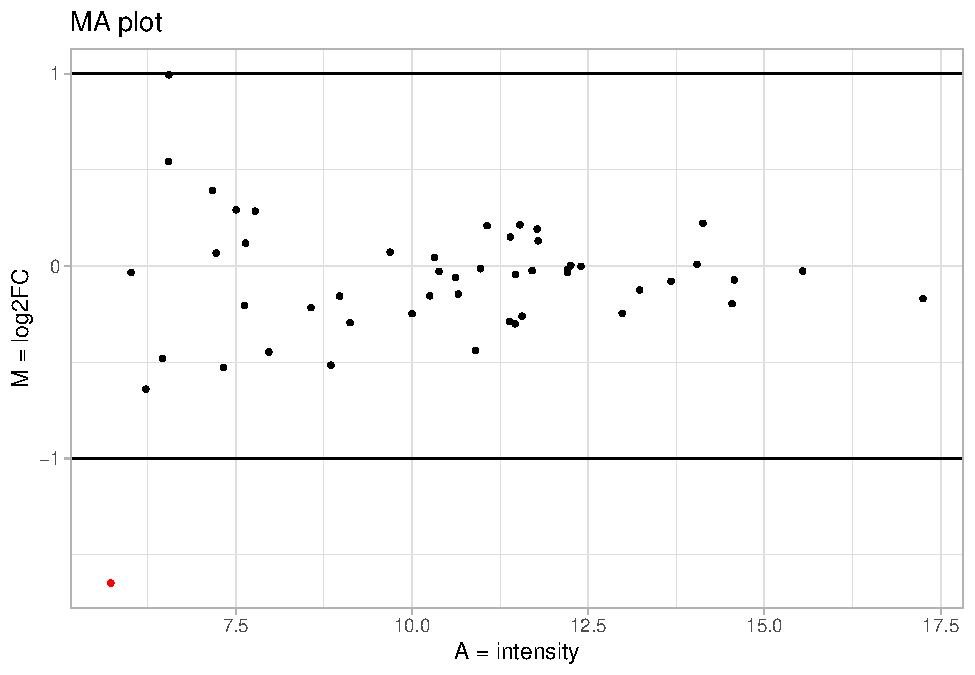
\includegraphics{_main_files/figure-latex/unnamed-chunk-114-1.pdf}

\hypertarget{plotly}{%
\section{Plotly}\label{plotly}}

\hypertarget{a-partir-de-ggplot2}{%
\subsection{A partir de ggplot2}\label{a-partir-de-ggplot2}}

\begin{Shaded}
\begin{Highlighting}[]
\FunctionTok{library}\NormalTok{(plotly)}
\FunctionTok{ggplotly}\NormalTok{(g)}
\end{Highlighting}
\end{Shaded}

\begin{verbatim}
## Warning: `gather_()` was deprecated in tidyr 1.2.0.
## i Please use `gather()` instead.
## i The deprecated feature was likely used in the plotly package.
##   Please report the issue at <https://github.com/plotly/plotly.R/issues>.
\end{verbatim}

\hypertarget{en-plotly-pur}{%
\subsection{En plotly pur}\label{en-plotly-pur}}

\begin{Shaded}
\begin{Highlighting}[]
\FunctionTok{plot\_ly}\NormalTok{(}\AttributeTok{data =}\NormalTok{ exprs\_annot, }\AttributeTok{x =} \SpecialCharTok{\textasciitilde{}}\NormalTok{A, }\AttributeTok{y =} \SpecialCharTok{\textasciitilde{}}\NormalTok{M, }\AttributeTok{text =} \FunctionTok{paste}\NormalTok{(}\StringTok{"Gene name :"}\NormalTok{, exprs\_annot}\SpecialCharTok{$}\NormalTok{name), }\AttributeTok{type =} \StringTok{\textquotesingle{}scatter\textquotesingle{}}\NormalTok{, }\AttributeTok{mode =} \StringTok{\textquotesingle{}markers\textquotesingle{}}\NormalTok{)}
\end{Highlighting}
\end{Shaded}

\hypertarget{echarts}{%
\section{echarts}\label{echarts}}

\begin{Shaded}
\begin{Highlighting}[]
\FunctionTok{library}\NormalTok{(echarts4r)}
\FunctionTok{library}\NormalTok{(dplyr)}

\NormalTok{exprs  }\SpecialCharTok{\%\textgreater{}\%}
  \FunctionTok{mutate}\NormalTok{(}\AttributeTok{interst =} \FunctionTok{ifelse}\NormalTok{(}\FunctionTok{abs}\NormalTok{(M) }\SpecialCharTok{\textless{}=} \DecValTok{1}\NormalTok{, }\DecValTok{1}\NormalTok{,}\DecValTok{2}\NormalTok{))}\SpecialCharTok{|\textgreater{}} 
  \FunctionTok{group\_by}\NormalTok{(interst)}\SpecialCharTok{|\textgreater{}}          
  \FunctionTok{e\_charts}\NormalTok{(A) }\SpecialCharTok{|\textgreater{}} 
  \FunctionTok{e\_scatter}\NormalTok{(M, }\AttributeTok{symbol\_size=}\DecValTok{10}\NormalTok{) }\SpecialCharTok{|\textgreater{}} 
  \FunctionTok{e\_legend}\NormalTok{(}\ConstantTok{FALSE}\NormalTok{) }\SpecialCharTok{|\textgreater{}}
  \FunctionTok{e\_tooltip}\NormalTok{() }\SpecialCharTok{|\textgreater{}}
  \FunctionTok{e\_color}\NormalTok{(}
    \FunctionTok{c}\NormalTok{(}\StringTok{"black"}\NormalTok{, }\StringTok{"red"}\NormalTok{)}
\NormalTok{  ) }\SpecialCharTok{|\textgreater{}}
  \FunctionTok{e\_title}\NormalTok{(}\StringTok{"MA plot"}\NormalTok{) }\SpecialCharTok{|\textgreater{}}
  \FunctionTok{e\_axis\_labels}\NormalTok{(}\AttributeTok{y =} \StringTok{"M = log2FC"}\NormalTok{, }\AttributeTok{x =} \StringTok{"A = intensity"}\NormalTok{) }\SpecialCharTok{|\textgreater{}}
  \FunctionTok{e\_toolbox\_feature}\NormalTok{(}\AttributeTok{feature =} \StringTok{"saveAsImage"}\NormalTok{)  }\SpecialCharTok{|\textgreater{}}
  \FunctionTok{e\_toolbox\_feature}\NormalTok{(}\AttributeTok{feature =} \StringTok{"dataZoom"}\NormalTok{)  }\SpecialCharTok{|\textgreater{}}
  \FunctionTok{e\_toolbox\_feature}\NormalTok{(}\AttributeTok{feature =} \StringTok{"dataView"}\NormalTok{)}
\end{Highlighting}
\end{Shaded}

\hypertarget{conclusion}{%
\chapter{Conclusion}\label{conclusion}}

\hypertarget{take-home-messages}{%
\section{Take home messages}\label{take-home-messages}}

\begin{itemize}
\tightlist
\item
  Tout est faisable avec R
\item
  \textbf{Définir et comprendre l'opération mathématique/statistique} avant de chercher la fonction R correspondante
\item
  R est un langage :

  \begin{itemize}
  \tightlist
  \item
    plusieurs types et structures de données (out of scope)
  \item
    énormément de commandes à découvrir (out of scope)
  \item
    Google est votre ami
  \end{itemize}
\item
  Une infinité de :

  \begin{itemize}
  \tightlist
  \item
    ressources en ligne
  \item
    tutoriels pour des analyses spécifiques (e.g.~DESeq2 pour le RNA-Seq)
  \end{itemize}
\end{itemize}

Bonnes pratiques : \url{https://style.tidyverse.org/syntax.html}

\hypertarget{ressources-ifb}{%
\section{Ressources IFB}\label{ressources-ifb}}

\begin{itemize}
\tightlist
\item
  Serveur RStudio: \url{https://rstudio.cluster.france-bioinformatique.fr/}
\item
  Jupyter lab (inclut un serveur RStudio et plein d'autres choses : \url{http://jupyterhub.cluster.france-bioinformatique.fr/}
\item
  Une question ? Un besoin ? Un problème ? Contactez la communauté IFB : \url{https://community.france-bioinformatique.fr/}
\end{itemize}

\hypertarget{resource}{%
\section{Resource}\label{resource}}

\begin{itemize}
\tightlist
\item
  R : \url{https://www.r-project.org/}
\item
  RStudio : \url{https://rstudio.com/}
\item
  R bloggers : \url{https://www.r-bloggers.com/}
\item
  Thinkr : \url{https://thinkr.fr/}
\item
  Rstudio Cheatsheets (un tas de thèmes): \url{https://rstudio.com/resources/cheatsheets/}
\end{itemize}

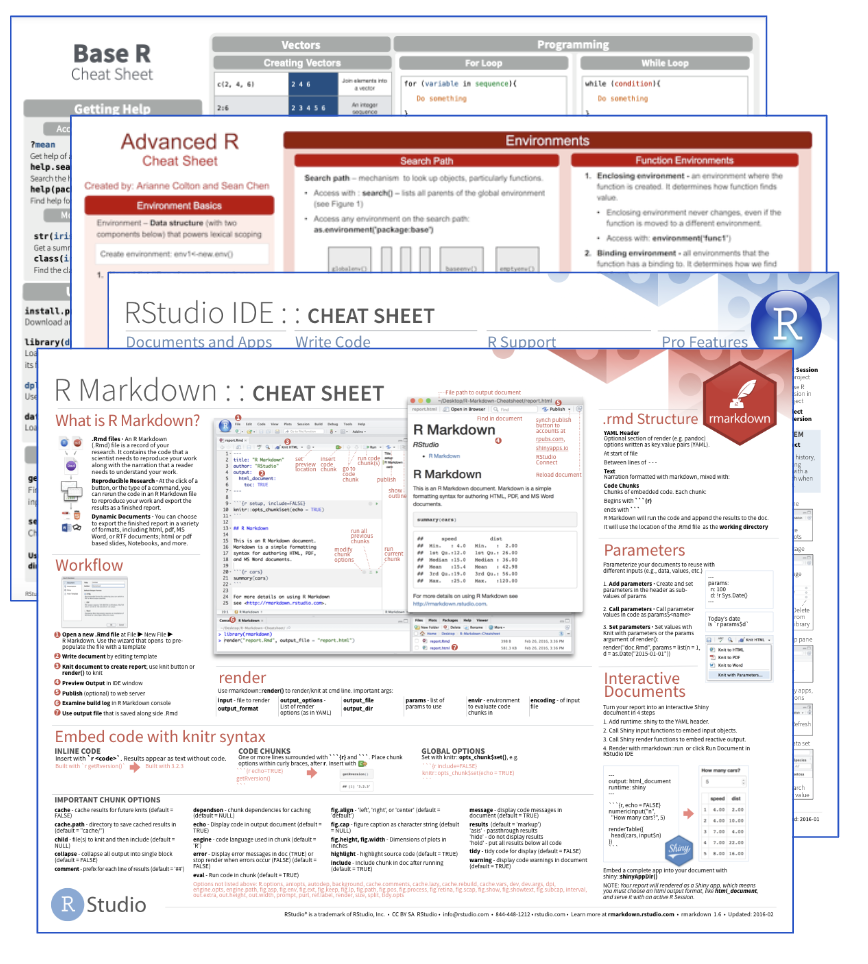
\includegraphics{images/cheatSheet.png}

  \bibliography{book.bib,packages.bib}

\end{document}
